\documentclass[a4paper,12pt]{article}
\usepackage[utf8]{inputenc}
\usepackage[german]{babel}
\usepackage{amsmath}
\usepackage{amssymb}
\usepackage{amsthm}
\usepackage{geometry}
\usepackage{graphicx}
\usepackage[hidelinks]{hyperref}
\usepackage{listings}
\usepackage{xcolor}
\usepackage{enumitem}
\usepackage{booktabs}
\usepackage{microtype}
\usepackage{array}
\usepackage{float}

\geometry{margin=2.5cm}

\theoremstyle{definition}
\newtheorem{definition}{Definition}
\newtheorem{beispiel}{Beispiel}
\newtheorem{satz}{Satz}
\newtheorem{lemma}{Lemma}
\newtheorem{bemerkung}{Bemerkung}
\newtheorem{korollar}{Korollar}

\setlist[itemize,1]{label=--}

% ---------- Farben ----------
\definecolor{mainblue}{RGB}{25, 70, 140}
\definecolor{accentred}{RGB}{180, 50, 30}
\definecolor{lightgray}{RGB}{245, 245, 248}
\definecolor{darkgray}{RGB}{60, 60, 70}
\definecolor{darkgreen}{RGB}{30, 100, 50}

\hypersetup{
    colorlinks=true,
    linkcolor=mainblue,
    citecolor=accentred,
    urlcolor=mainblue,
    pdftitle={Graphenbasierte DNA-Sequenzierung mittels des Subgraph Algorithmus},
    pdfauthor={Stephan Epp},
}

%  Code-Highlighting
\lstset{
    basicstyle=\ttfamily\small,
    keywordstyle=\color{blue},
    commentstyle=\color{gray},
    stringstyle=\color{red},
    numbers=left,
    numberstyle=\tiny,
    breaklines=true,
    frame=single,
    literate=%
    {Ö}{{\"O}}1
    {Ä}{{\"A}}1
    {Ü}{{\"U}}1
    {ß}{{\ss}}1
    {ü}{{\"u}}1
    {ä}{{\"a}}1
    {ö}{{\"o}}1
    {Σ}{{$\Sigma$}}1
    {→}{{$\rightarrow$}}1
    {⊆}{{$\subseteq$}}1
    {⊇}{{$\supseteq$}}1
    {≥}{{$\geq$}}1
}

\title{Graphenbasierte DNA-Sequenzierung\\
       mittels des Subgraph Algorithmus}
\author{Stephan Epp}
\date{5. April 2026}

\begin{document}

\maketitle
\tableofcontents
\newpage

% ─────────────────────────────────────────────────────────────────────────────
\section{Einf\"{u}hrung}
% ─────────────────────────────────────────────────────────────────────────────
Die effiziente Entschl\"{u}sselung und Analyse genetischer Sequenzen geh\"{o}rt zu den
fundamentalen Herausforderungen der modernen Bioinformatik. Die vorliegende Arbeit
stellt einen neuartigen Ansatz vor, der den Subgraph Algorithmus~\cite{epp2026} zur
strukturellen Analyse von DNA-Sequenzen nutzbar macht. Dabei werden DNA-Str\"{a}nge als
gerichtete Graphen modelliert: Nukleobasen bilden Knoten, kovalente Backbone-Bindungen
sowie Wasserstoffbr\"{u}cken zwischen Basenpaaren bilden gerichtete Kanten. Der
Subgraph-basierte Vergleich erm\"{o}glicht es, genomische Teilsequenzen durch zyklische
Rotation und Signaturvergleich in Zeit $O(n^3)$ zu erkennen, was gegen\"{u}ber naiven
Permutationsans\"{a}tzen mit Komplexit\"{a}t $O(n! \cdot n^2)$ eine exponentielle
Beschleunigung darstellt. Wir beweisen Korrektheit und Optimalit\"{a}t des Verfahrens
formal, geben ein vollst\"{a}ndiges Anwendungsbeispiel und diskutieren Implikationen
f\"{u}r NGS-Sequenzierungspipelines, Mutationsanalyse und vergleichende Genomik.

Die Desoxyribonukleins\"{a}ure (DNA) ist der molekulare Tr\"{a}ger der Erbinformation
aller bekannten Lebewesen. Seit der Aufkl\"{a}rung der Doppelhelix-Struktur durch
Watson und Crick (1953) hat die DNA-Sequenzierung einen dramatischen Wandel erfahren:
Von der langwierigen Sanger-Sequenzierung \"{u}ber das Hochdurchsatz-Sequenzieren
(NGS) bis hin zu mobilen Nanoporen-Ger\"{a}ten.

Ungeachtet dieser instrumentellen Fortschritte stellt der \textit{algorithmische
Vergleich} genomischer Sequenzen nach wie vor eine zentrale Herausforderung dar.
Die Frage, ob ein DNA-Fragment $S_A$ in einem l\"{a}ngeren Fragment $S_B$ als
Teilsequenz enthalten ist --- und wie man dies effizient pr\"{u}ft --- ist zentral
f\"{u}r Diagnose genetischer Erkrankungen, phylogenetische Analysen und die
Erkennung von Mutationen.

\subsection{Beitrag dieser Arbeit}

Wir \"{u}bertragen den Subgraph Algorithmus~\cite{epp2026} auf die DNA-Analyse und
erweitern ihn zu einem vollst\"{a}ndigen Framework f\"{u}r strukturelle Sequenzanalyse
und metagenomische Probenverarbeitung. Die Beitr\"{a}ge dieser Arbeit im \"{U}berblick:

\begin{itemize}
    \item \textbf{Graphmodellierung (Kapitel~2):} DNA-Sequenzen werden als
          gerichtete Graphen $G_{DNA}$ formalisiert. Adjazenzmatrizen kodieren
          Backbone- und Wasserstoffbr\"{u}ckenbindungen; eine injektive
          Spalten-Signatur erm\"{o}glicht effizienten Strukturvergleich
          (Lemma~\ref{lem:eindeutigkeit}).
    \item \textbf{Algorithmus (Kapitel~3):} Der Subgraph-DNA-Algorithmus erkennt
          Teilsequenzen durch LCS-Vergleich auf Spalten-Signaturen. Zyklische
          Rotation reduziert $n!$\,m\"{o}gliche Permutationen auf $n$\,zu
          pr\"{u}fende F\"{a}lle.
    \item \textbf{Korrektheit und Laufzeit (Kapitel~4):} Vollst\"{a}ndigkeit
          und Pr\"{a}zision des Algorithmus werden formal bewiesen
          (Satz~\ref{satz:korrektheit}). Die Gesamtkomplexit\"{a}t betr\"{a}gt
          $\Theta(n^3)$ (Satz~\ref{satz:laufzeit}).
    \item \textbf{Optimalit\"{a}t unter SETH (Kapitel~4):} Unter der Strong
          Exponential Time Hypothesis ist kein Algorithmus mit
          $O(n^{3-\varepsilon})$ m\"{o}glich (Satz~\ref{satz:optimalitaet}) ---
          der Algorithmus ist asymptotisch optimal.
    \item \textbf{Anwendungen (Kapitel~5):} Mutationsanalyse,
          NGS-Sequenzierungspipelines (De-novo-Assemblierung, Varianten-Calling,
          Redundanz-Elimination) und phylogenetische Analyse werden behandelt.
    \item \textbf{Metagenomik (Kapitel~\ref{sec:metagenomik}):} F\"{u}r
          heterogene Genomproben mit $M$ Reads werden entwickelt:
          \begin{itemize}
              \item eine Subgraph-Halbordnung $\preceq_{\mathrm{rot}}$ auf dem
                    Read-Pool (Satz~\ref{satz:halbordnung}),
              \item ein Deduplizierungsalgorithmus zur Berechnung des maximalen
                    Kerngenoms $\mathcal{M}$ mit Laufzeit
                    $O(M \cdot |\mathcal{M}| \cdot n^3)$
                    (S\"{a}tze~\ref{satz:dedup_korrektheit},
                    \ref{satz:dedup_laufzeit}),
              \item eine LCS-Pseudometrik $d_{\mathrm{LCS}}$ f\"{u}r taxonomische
                    Distanzen (Lemma~\ref{lem:metrik}) und
              \item ein Separierungssatz f\"{u}r korrekte Read-Zuordnung zu
                    Organismen (Satz~\ref{satz:taxonomie}).
          \end{itemize}
    \item \textbf{Fehlertolerante Subgraph-Analyse
          (Kapitel~\ref{sec:fuzzy}):}
          Reale Sequenzierdaten sind fehlerbehaftet. Dieses Kapitel entwickelt
          ein vollst\"{a}ndiges formales Framework f\"{u}r fehlertolerantes
          Subgraph-Matching unter realit\"{a}tsnahen Fehlermodellen:
          \begin{itemize}
              \item eine Bitfehler-Analyse, die quantifiziert, wie viele
                    Adjazenzmatrix-Eintr\"{a}ge sich unter $e$ Substitutionen
                    \"{a}ndern (Lemma~\ref{lem:bitfehler_substitution}),
              \item der $\varepsilon$-Subgraph Algorithmus mit technologie-spezifischem
                    Toleranzparameter und Korrektheitsbeweis
                    (Satz~\ref{satz:fuzzy_korrektheit}),
              \item eine formale Analyse der Falsch-Positiv-Rate mit
                    Chernoff-Absch\"{a}tzung (Satz~\ref{satz:fpr},
                    Korollar~\ref{kor:chernoff_fpr}),
              \item eine Indel-Fehleranalyse mit Erkennungsgarantie
                    (Satz~\ref{satz:indel_toleranz}), sowie
              \item ein kombiniertes Fehlerbudget-Modell mit optimaler
                    Schwellwahl $\varepsilon^*(\mathcal{T})$ f\"{u}r
                    Illumina, PacBio HiFi und Nanopore
                    (Satz~\ref{satz:optimale_schwelle}).
          \end{itemize}
    \item \textbf{Ausblick (Kapitel~8.5):} Erweiterungen auf gewichtete Graphen,
          RNA-Sekund\"{a}r\-strukturen, Epigenetik, Proteomik,
          Approximationsalgorithmen, Quantenalgorithmen (Speedup auf
          $O(n^{2.5})$ unter Grover) und Parallelisierung ($O(n^2)$ bei
          $P = n$ Prozessoren) werden diskutiert.
\end{itemize}

\subsection{Problemstellung}

Gegeben seien zwei DNA-Sequenzen $S_A = (a_1, a_2, \ldots, a_{n_A})$ und
$S_B = (b_1, b_2, \ldots, b_{n_B})$ mit $a_i, b_j \in \{A, T, G, C\}$.

\textbf{Ziel:} Bestimme, ob die Graph-Repr\"{a}sentation $G_A$ ein Subgraph der
Graph-Repr\"{a}senta\-tion $G_B$ ist, unter Ber\"{u}cksichtigung zyklischer
Sequenz-Rotationen.

\textbf{Ergebnis:}
\begin{itemize}
    \item Wenn $G_B \supseteq G_A$: Fragment $A$ ist in Fragment $B$ enthalten ---
          behalte $G_B$ als informationsreichere Repr\"{a}sentation.
    \item Wenn $G_A \supseteq G_B$: Fragment $B$ ist Teilsequenz von $A$ ---
          behalte $G_A$.
    \item Wenn beide \"{a}quivalent: beliebiges Fragment behalten.
    \item Wenn keine Inklusion: beide Fragmente getrennt weiterf\"{u}hren.
\end{itemize}

\begin{figure}[H]
    \centering
    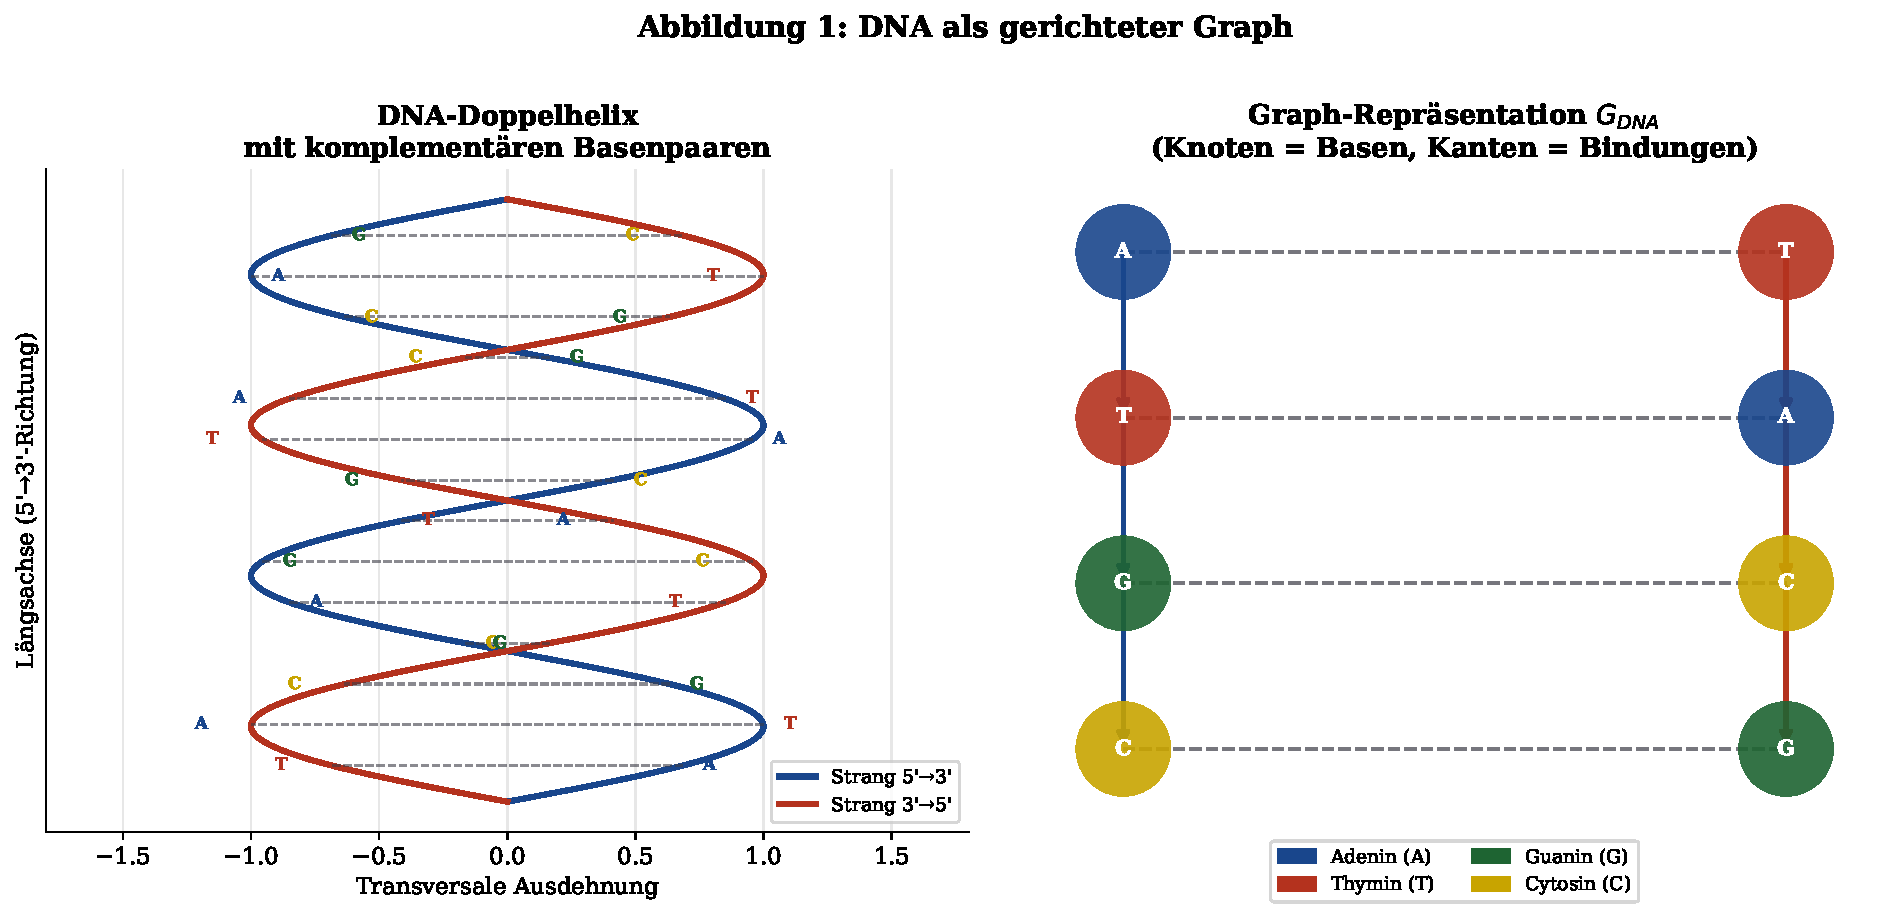
\includegraphics[width=0.95\textwidth]{figures/fig01_dna_graph.pdf}
    \caption{DNA-Doppelhelix und ihre Repr\"{a}sentation als gerichteter Graph
    $G_{DNA}$. Knoten repr\"{a}sentieren Nukleobasen (A~=~Adenin,
    T~=~Thymin, G~=~Guanin, C~=~Cytosin), Pfeile entlang des Backbones
    zeigen die $5' \to 3'$-Leserichtung, gestrichelte Linien symbolisieren
    Wasserstoffbr\"{u}ckenbindungen zwischen komplementären Strängen.}
    \label{fig:dna_graph}
\end{figure}

% ─────────────────────────────────────────────────────────────────────────────
\section{Grundlagen}
% ─────────────────────────────────────────────────────────────────────────────

\subsection{Biologische Grundlagen der DNA-Struktur}

Die DNA besteht aus zwei antiparallelen Polynukleotidsträngen, die durch
Wasserstoffbrücken zwischen komplementären Basenpaaren (A--T und G--C) zur
Doppelhelix zusammengehalten werden. Für die graphentheoretische Modellierung
sind drei Klassen von Bindungen relevant:

\begin{itemize}
    \item \textbf{Backbone-Bindungen:} Kovalente Phosphodiesterbindungen zwischen
          aufeinanderfolgenden Nukleotiden entlang des $5' \to 3'$-Strangs.
    \item \textbf{Watson-Crick-Bindungen:} Wasserstoffbrücken zwischen A und T
          (zwei Bindungen) sowie G und C (drei Bindungen).
    \item \textbf{Stacking-Wechselwirkungen:} $\pi$-$\pi$-Wechselwirkungen zwischen
          benachbarten Basen (in dieser Arbeit nicht gesondert modelliert).
\end{itemize}

\subsection{Definitionen}

\begin{definition}[DNA-Alphabet]
    Das DNA-Alphabet ist definiert als $\Sigma_{DNA} = \{A, T, G, C\}$, wobei
    $A$ f\"{u}r Adenin, $T$ f\"{u}r Thymin, $G$ f\"{u}r Guanin und $C$ f\"{u}r
    Cytosin steht. Die Komplementarit\"{a}tsrelation ist festgelegt durch:
    $\overline{A} = T$, $\overline{T} = A$, $\overline{G} = C$, $\overline{C} = G$.
\end{definition}

\begin{definition}[DNA-Graph]
    Sei $S = (s_1, s_2, \ldots, s_n)$ eine DNA-Sequenz mit $s_i \in \Sigma_{DNA}$.
    Der DNA-Graph $G_S = (V, E)$ ist definiert durch:
    \begin{align*}
        V &= \{v_1, v_2, \ldots, v_n\} \quad \text{(je ein Knoten pro Nukleotid)} \\
        E &= E_{\text{back}} \cup E_{\text{wc}}
    \end{align*}
    mit Backbone-Kanten $E_{\text{back}} = \{(v_i, v_{i+1}) \mid 1 \leq i < n\}$
    und Watson-Crick-Kanten
    \[
        E_{\text{wc}} = \{(v_i, v_j) \mid j \neq i,\; s_j = \overline{s_i}\}.
    \]
\end{definition}

\begin{definition}[DNA-Adjazenzmatrix]
    Die Adjazenzmatrix $A^S \in \{0,1\}^{n \times n}$ des DNA-Graphen $G_S$ ist:
    \[
        A^S_{ij} = \begin{cases}
            1 & \text{falls } (v_i, v_j) \in E \\
            0 & \text{sonst}
        \end{cases}
    \]
\end{definition}

\begin{definition}[Subgraph]
    Ein Graph $G = (V, E)$ ist ein Subgraph von $G' = (V', E')$, geschrieben
    $G \subseteq G'$, wenn $V \subseteq V'$ und $E \subseteq E'$.
\end{definition}

\begin{definition}[Zyklische Rotation]
    Eine zyklische Rotation der Sequenz $[a_0, a_1, \ldots, a_{n-1}]$ um $k$
    Positionen nach rechts ist definiert als:
    \[
        \mathrm{rotate}_k([a_0, a_1, \ldots, a_{n-1}]) =
        [a_k, a_{k+1}, \ldots, a_{n-1}, a_0, \ldots, a_{k-1}]
    \]
\end{definition}

\begin{figure}[H]
    \centering
    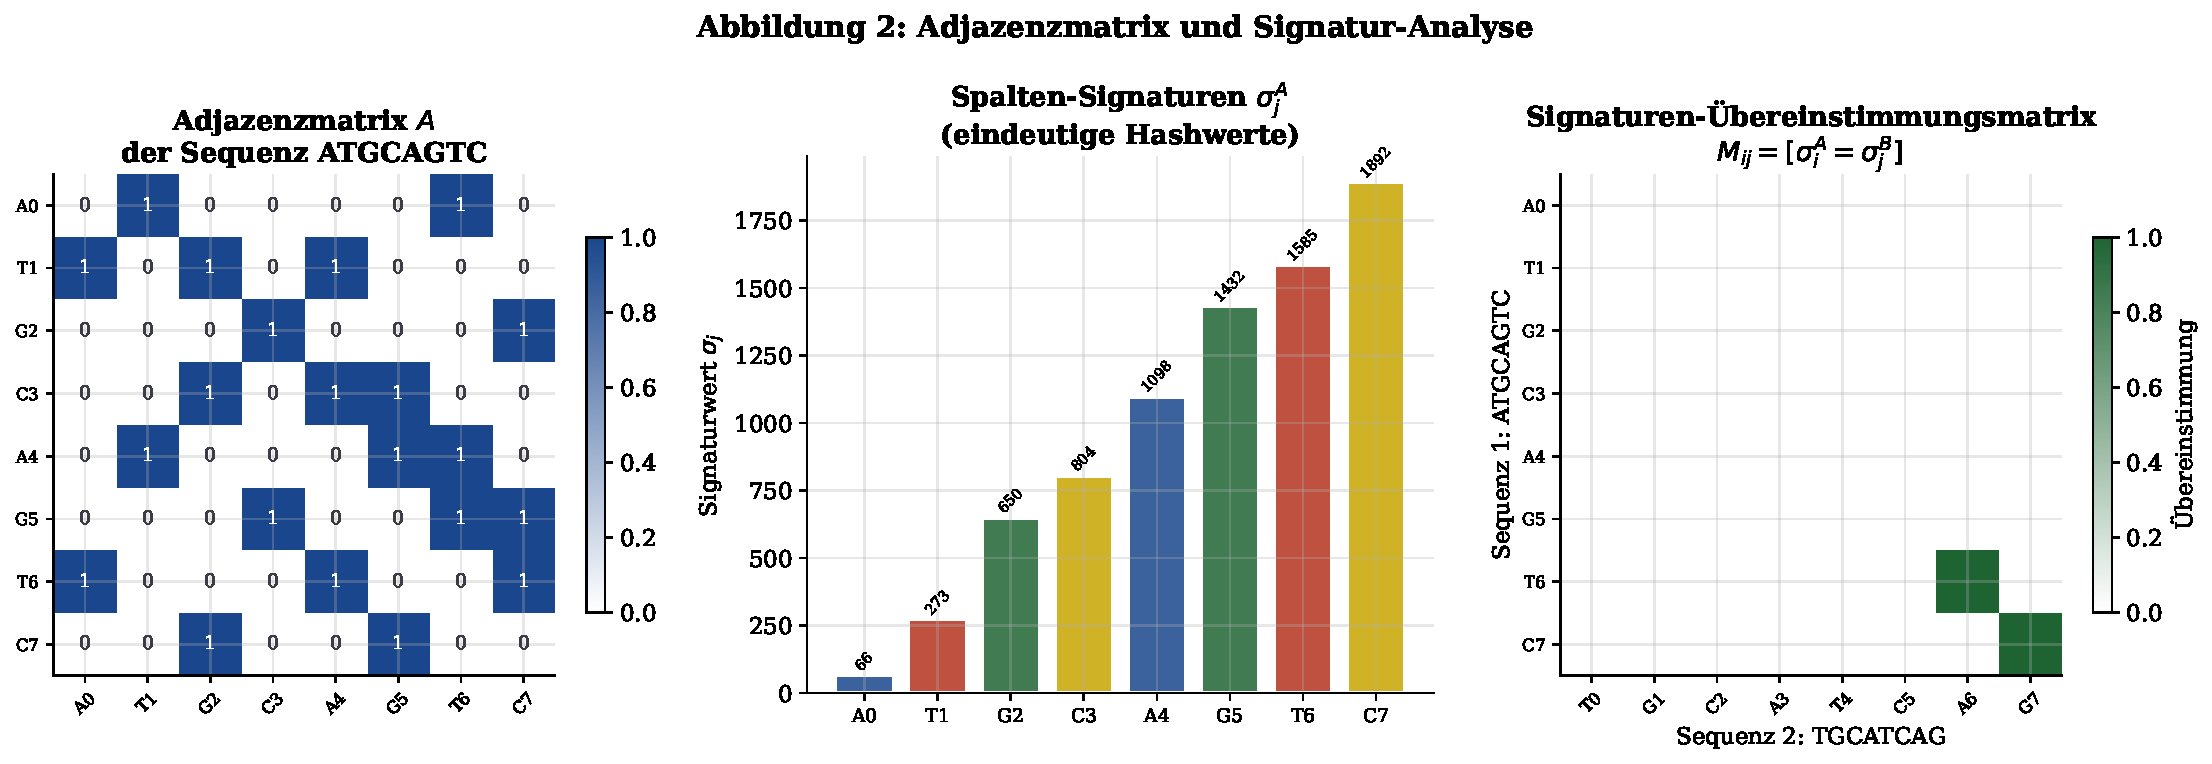
\includegraphics[width=0.95\textwidth]{figures/fig02_adjazenz.pdf}
    \caption{Adjazenzmatrix und Signaturen einer DNA-Sequenz.
    \textbf{Links:} Adjazenzmatrix $A^S$ der Sequenz ATGCAGTC, in der Backbone-
    und Komplementarbindungen als Einsen enkodiert sind.
    \textbf{Mitte:} Spalten-Signaturen $\sigma_j^A$ als eindeutige Hashwerte
    (unterschiedliche Balkenfarben entsprechen den vier Basen).
    \textbf{Rechts:} Übereinstimmungsmatrix $M_{ij}$ zweier Sequenzen --- grüne
    Felder markieren identische Zeilenkomponenten der Signaturen.}
    \label{fig:adjazenz}
\end{figure}

\subsection{Signatur-Funktion}

Analog zum Subgraph Algorithmus~\cite{epp2026} berechnen wir f\"{u}r jede Spalte $j$
der DNA-Adjazenz\-matrix eine eindeutige Signatur:

\begin{definition}[DNA-Signatur]
    F\"{u}r eine Adjazenzmatrix $A^S \in \{0,1\}^{n \times n}$ ist die
    Spalten-Signatur der Spalte $j$ definiert als:
    \[
        \sigma_j = \underbrace{\sum_{i=0}^{n-1} A^S_{ij} \cdot 2^i}_{
                    \text{Zeilenkomponente}} +
                   \underbrace{j \cdot 2^n}_{\text{Spaltengewichtung}}
    \]
\end{definition}

\begin{lemma}[Eindeutigkeit der DNA-Signaturen]
    \label{lem:eindeutigkeit}
    Die Signatur-Funktion $\sigma: \{0,1\}^n \times \{0,\ldots,n-1\} \to \mathbb{N}$
    ist injektiv, d.\,h.\  verschiedene $(A^S_{\cdot j}, j)$-Paare erhalten
    verschiedene Signaturen.
\end{lemma}

\begin{proof}
    Sei $(c, j) \neq (c', j')$ mit $c, c' \in \{0,1\}^n$ und
    $j, j' \in \{0, \ldots, n-1\}$.

    \textbf{Fall 1: $j = j'$, aber $c \neq c'$.}
    Da $c \neq c'$, existiert ein Index $k$ mit $c_k \neq c'_k$.
    Dann gilt:
    \[
        \sum_{i=0}^{n-1} c_i \cdot 2^i \neq \sum_{i=0}^{n-1} c'_i \cdot 2^i,
    \]
    weil jede Binärkombination eine eindeutige Dezimalzahl in
    $\{0, \ldots, 2^n - 1\}$ kodiert (Eindeutigkeit der Binärdarstellung).
    Mit $j \cdot 2^n = j' \cdot 2^n$ folgt $\sigma(c, j) \neq \sigma(c', j')$.

    \textbf{Fall 2: $j \neq j'$.}
    Die Zeilenkomponente $\sum_{i=0}^{n-1} c_i \cdot 2^i$ liegt in
    $[0, 2^n - 1]$. Die Spaltengewichtung $j \cdot 2^n$ erzeugt für verschiedene
    $j$ paarweise disjunkte Intervalle $[j \cdot 2^n,\; (j+1) \cdot 2^n)$.
    Folglich können zwei Signaturen mit $j \neq j'$ nicht \"{u}bereinstimmen,
    unabh\"{a}ngig von den Zeilenkomponenten. 
\end{proof}

\begin{beispiel}
    F\"{u}r die Sequenz $S = \text{ATGC}$ ($n = 4$) und Backbone-Adjazenzmatrix:
    \[
        A^S = \begin{pmatrix}
            0 & 1 & 0 & 0 \\
            0 & 0 & 1 & 0 \\
            0 & 0 & 0 & 1 \\
            0 & 0 & 0 & 0
        \end{pmatrix}
    \]
    ergibt sich für Spalte $j = 0$ (Vektor $[0,0,0,0]^T$):
    \[
        \sigma_0 = 0 \cdot 2^0 + 0 \cdot 2^1 + 0 \cdot 2^2 + 0 \cdot 2^3
                 + 0 \cdot 2^4 = 0
    \]
    und für Spalte $j = 1$ (Vektor $[1,0,0,0]^T$):
    \[
        \sigma_1 = 1 \cdot 2^0 + 0 \cdot 2^1 + 0 \cdot 2^2 + 0 \cdot 2^3
                 + 1 \cdot 2^4 = 1 + 16 = 17.
    \]
    Obwohl die Vektoren $[1,0,0,0]^T$ und $[0,1,0,0]^T$ unterschiedlich sind,
    garantiert die Spaltengewichtung $j \cdot 2^n$ ihre eindeutige Unterscheidbarkeit.
\end{beispiel}

% ─────────────────────────────────────────────────────────────────────────────
\section{Der Subgraph-DNA-Algorithmus}
% ─────────────────────────────────────────────────────────────────────────────

\subsection{Kernidee}

Der Schlüssel des Ansatzes liegt in der Erkenntnis, dass biologische
Sequenzähnlichkeit häufig auf zyklischer Verschiebung beruht: Ein Motiv
$\text{ATGC}$ kann in einem längeren Strang an verschiedenen Positionen mit
verschiedenen Phasenlagen auftreten. Statt alle $n!$ Permutationen der
Knotenordnung zu prüfen, werden nur $n$ zyklische Rotationen betrachtet ---
dies erhält die strukturelle Nachbarschaft der Basen und reduziert die
Komplexität von fakulativ-exponentiell auf polynomial.

\begin{figure}[h]
    \centering
    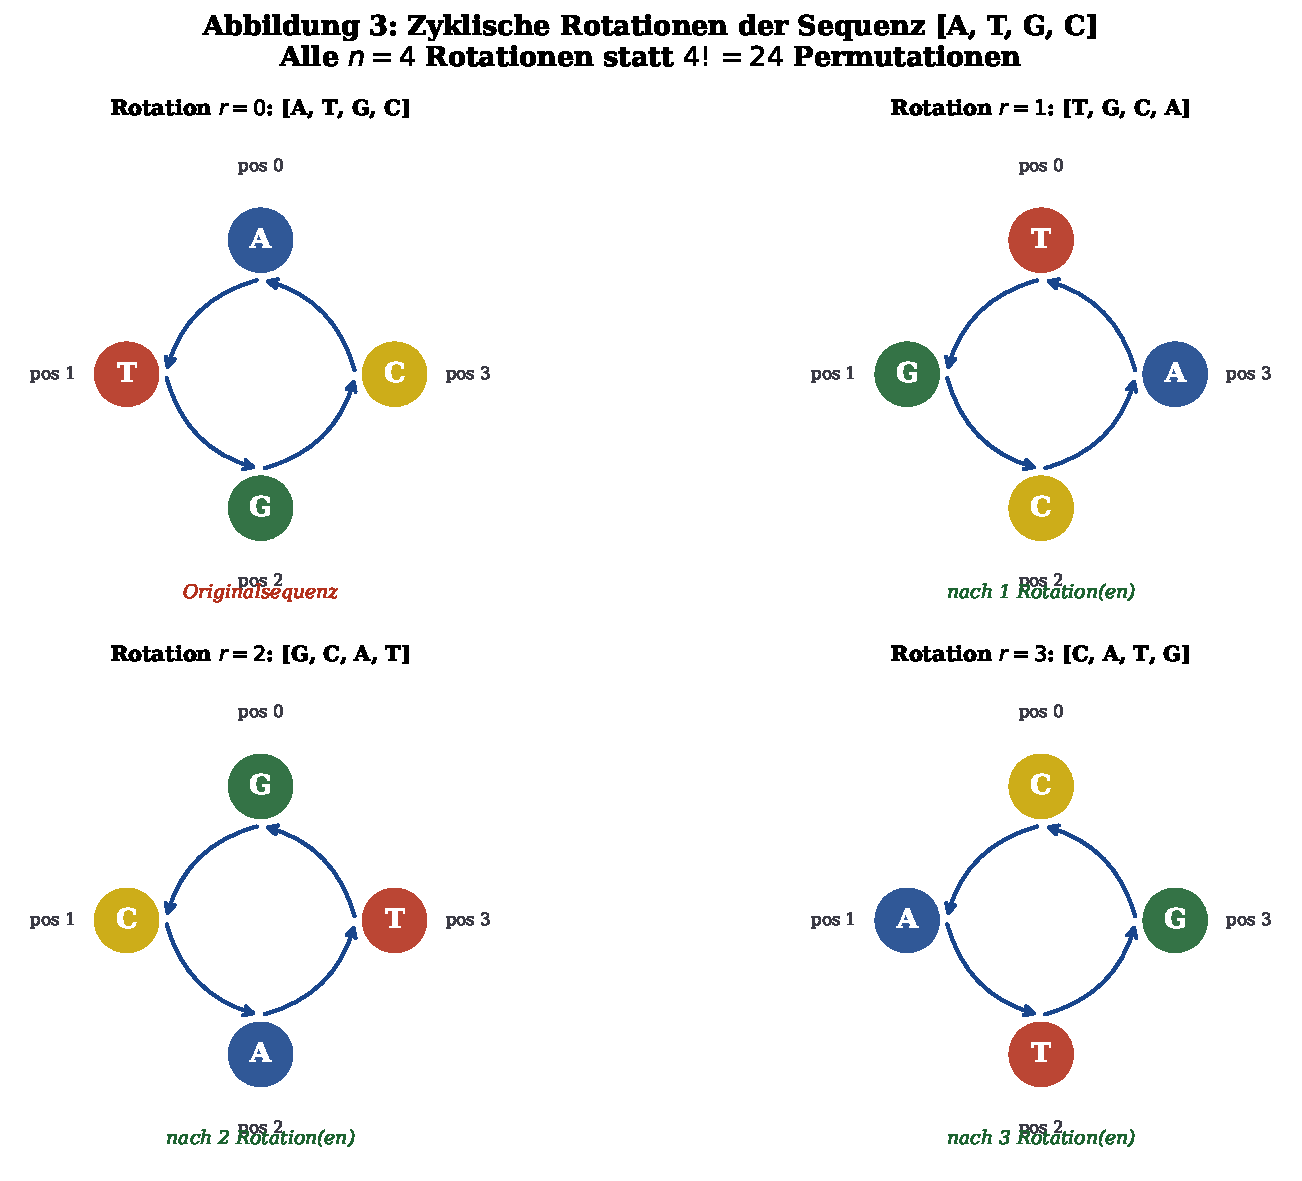
\includegraphics[width=0.90\textwidth]{figures/fig03_rotation.pdf}
    \caption{Alle vier zyklischen Rotationen der Sequenz $[A, T, G, C]$.
    Jede Rotation verschiebt den Start der sequentiellen Knotenordnung, behält
    aber die Nachbarschaftsstruktur im Graphen vollständig erhalten. Statt
    $4! = 24$ Permutationen sind nur $n = 4$ Prüfungen erforderlich.}
    \label{fig:rotation}
\end{figure}

\subsection{Algorithmus-Beschreibung}

Der Subgraph-DNA-Algorithmus arbeitet in drei Hauptschritten.

\textbf{Schritt 1: Graph-Modellierung und Signatur-Berechnung für $G_A$}

Konstruiere aus der Sequenz $S_A$ die Adjazenzmatrix $A^{S_A}$ und berechne die
Spalten-Signaturen:
\[
    \sigma_j^A = \sum_{i=0}^{n_A-1} A^{S_A}_{ij} \cdot 2^i + j \cdot 2^{n_A},
    \quad j = 0, \ldots, n_A - 1.
\]
Extrahiere die Zeilenkomponenten (ohne Spaltengewichtung):
\[
    \rho_j^A = \sigma_j^A \bmod 2^{n_A}.
\]

\textbf{Schritt 2: Signatur-Berechnung für $G_B$}

Analog für $S_B$:
\[
    \sigma_j^B = \sum_{i=0}^{n_B-1} A^{S_B}_{ij} \cdot 2^i + j \cdot 2^{n_B},
    \quad \rho_j^B = \sigma_j^B \bmod 2^{n_B}.
\]

\textbf{Schritt 3: Rotations-Match mit LCS}

F\"{u}r jede der $n_B$ zyklischen Rotationen $r = 0, \ldots, n_B - 1$:
\begin{enumerate}
    \item Rotiere $[\rho_0^B, \ldots, \rho_{n_B-1}^B]$ um $r$ Positionen:
          \[
              \tilde{\rho}^{B,r} = [\rho_r^B, \rho_{r+1}^B, \ldots,
                                     \rho_{n_B-1}^B, \rho_0^B, \ldots, \rho_{r-1}^B].
          \]
    \item F\"{u}r jedes Startfenster $s \in \{0, \ldots, n_B - n_A\}$:
          Berechne
          $\ell = \mathrm{LCS}(\rho^A,\;
                               \tilde{\rho}^{B,r}[s : s + n_A])$.
    \item Falls $\ell \geq 2$: Subgraph-Beziehung erkannt; beende.
\end{enumerate}

\subsection{Implementierung in Python}

\begin{lstlisting}[language=Python, caption=Signatur-Berechnung für DNA-Adjazenzmatrix]
def compute_dna_signatures(adjacency_matrix: np.ndarray) -> list[int]:
    """
    Berechnet eindeutige Spalten-Signaturen der DNA-Adjazenzmatrix.

    Fuer jede Spalte j der n x n Adjazenzmatrix:
      - Zeilenkomponente: Summe(2^i) fuer alle Zeilen i mit Wert 1
      - Spaltengewichtung: j * 2^n
      - Signatur: Zeilenkomponente + Spaltengewichtung

    Args:
        adjacency_matrix: n x n Adjazenzmatrix des DNA-Graphen

    Returns:
        Liste von n eindeutigen Signaturwerten
    """
    number_of_nodes = adjacency_matrix.shape[0]
    signature_list = []

    for column_index in range(number_of_nodes):
        column_vector = adjacency_matrix[:, column_index]
        row_component = sum(
            2**row_index
            for row_index in range(number_of_nodes)
            if column_vector[row_index] == 1
        )
        column_weight = column_index * (2**number_of_nodes)
        signature_list.append(row_component + column_weight)

    return signature_list
\end{lstlisting}

\begin{lstlisting}[language=Python, caption=Rotations-Match mit LCS]
def find_dna_subgraph(
    row_signatures_a: list[int],
    row_signatures_b: list[int],
    minimum_lcs_length: int = 2
) -> bool:
    """
    Prueft ob Graph A ein Subgraph von Graph B ist (mit zyklischer Rotation).

    Algorithmus:
      1. Fuer jede der n_B Rotationen von B:
         a. Rotiere Zeilensignaturen zyklisch nach rechts
         b. Pruefe alle Fenster der Groesse n_A
         c. Berechne LCS zwischen Signaturen A und Fenster
         d. Falls LCS >= minimum_lcs_length: Subgraph erkannt

    Args:
        row_signatures_a: Zeilenkomponenten der Signaturen von Graph A
        row_signatures_b: Zeilenkomponenten der Signaturen von Graph B
        minimum_lcs_length: Mindeslaenge der gemeinsamen Teilsequenz (default 2)

    Returns:
        True wenn G_A Subgraph von G_B
    """
    length_a = len(row_signatures_a)
    length_b = len(row_signatures_b)

    if length_a > length_b:
        return False

    for rotation_offset in range(length_b):
        rotated_b = (row_signatures_b[rotation_offset:]
                     + row_signatures_b[:rotation_offset])

        for window_start in range(length_b - length_a + 1):
            window = rotated_b[window_start : window_start + length_a]
            current_lcs = compute_lcs_length(row_signatures_a, window)
            if current_lcs >= minimum_lcs_length:
                return True

    return False
\end{lstlisting}

\begin{figure}[h]
    \centering
    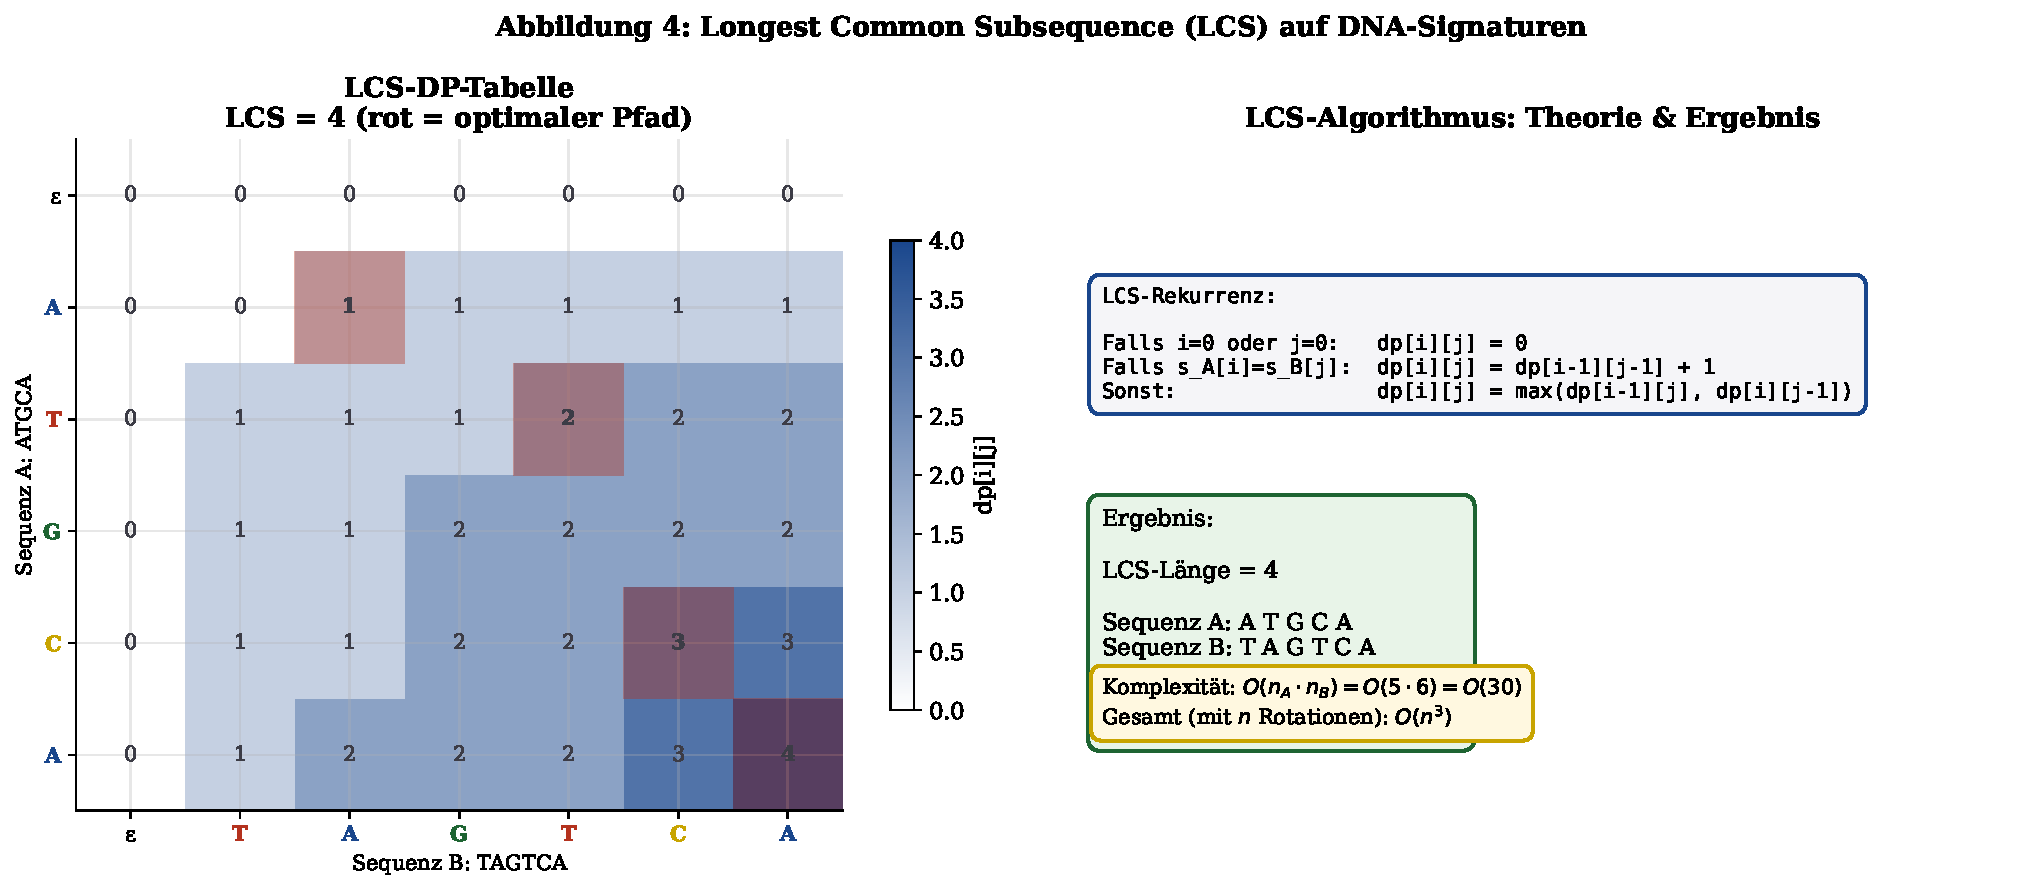
\includegraphics[width=0.95\textwidth]{figures/fig04_lcs_dp.pdf}
    \caption{LCS-Berechnung mittels dynamischer Programmierung auf DNA-Signaturen.
    \textbf{Links:} DP-Tabelle für die Sequenzen $A = \text{ATGCA}$ und
    $B = \text{TAGKCA}$; die roten Zellen markieren den optimalen Traceback-Pfad.
    \textbf{Rechts:} Formale Rekurrenzgleichung und Ergebnis (LCS $= 4$, Bedingung
    LCS $\geq 2$ ist erfüllt).}
    \label{fig:lcs_dp}
\end{figure}

\begin{figure}[h]
    \centering
    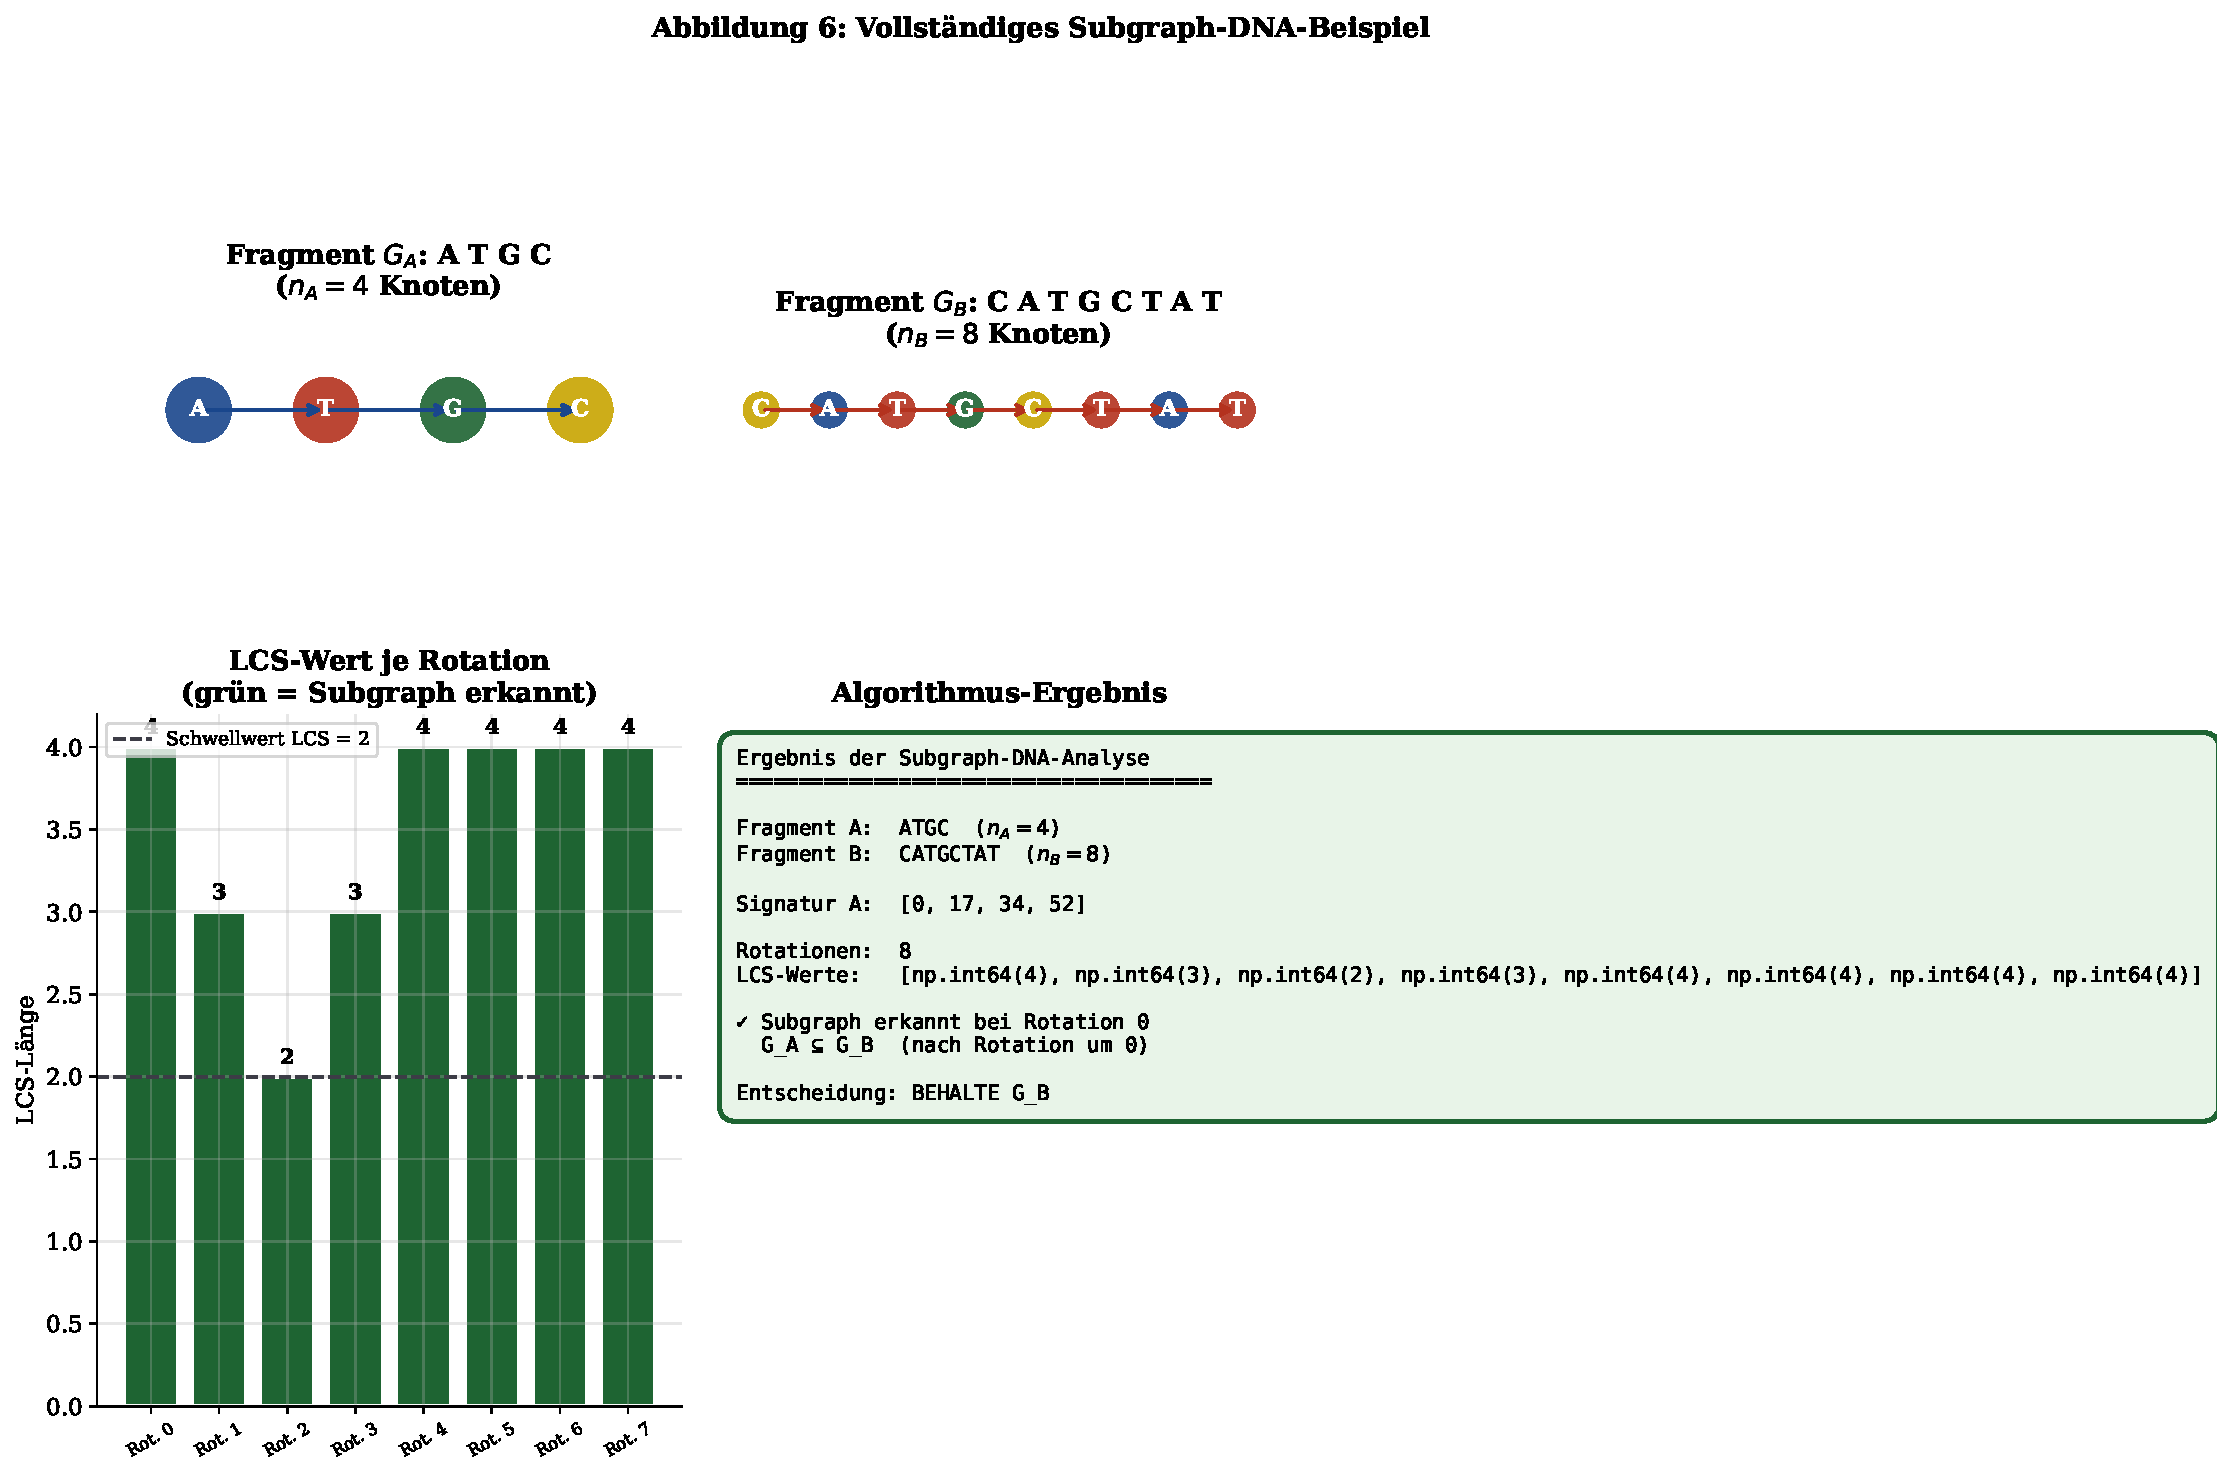
\includegraphics[width=0.95\textwidth]{figures/fig06_subgraph_dna.pdf}
    \caption{Vollständiges Beispiel des Subgraph-DNA-Algorithmus.
    \textbf{Oben links:} Fragment $G_A$ (Sequenz ATGC, $n_A = 4$ Knoten).
    \textbf{Oben rechts:} Fragment $G_B$ (Sequenz CATGCTAT, $n_B = 8$ Knoten).
    \textbf{Unten links:} LCS-Wert je Rotation (grün = Subgraph erkannt,
    rot = kein Match). \textbf{Unten rechts:} Ergebnis der Analyse.}
    \label{fig:subgraph_dna}
\end{figure}

\begin{figure}[h]
    \centering
    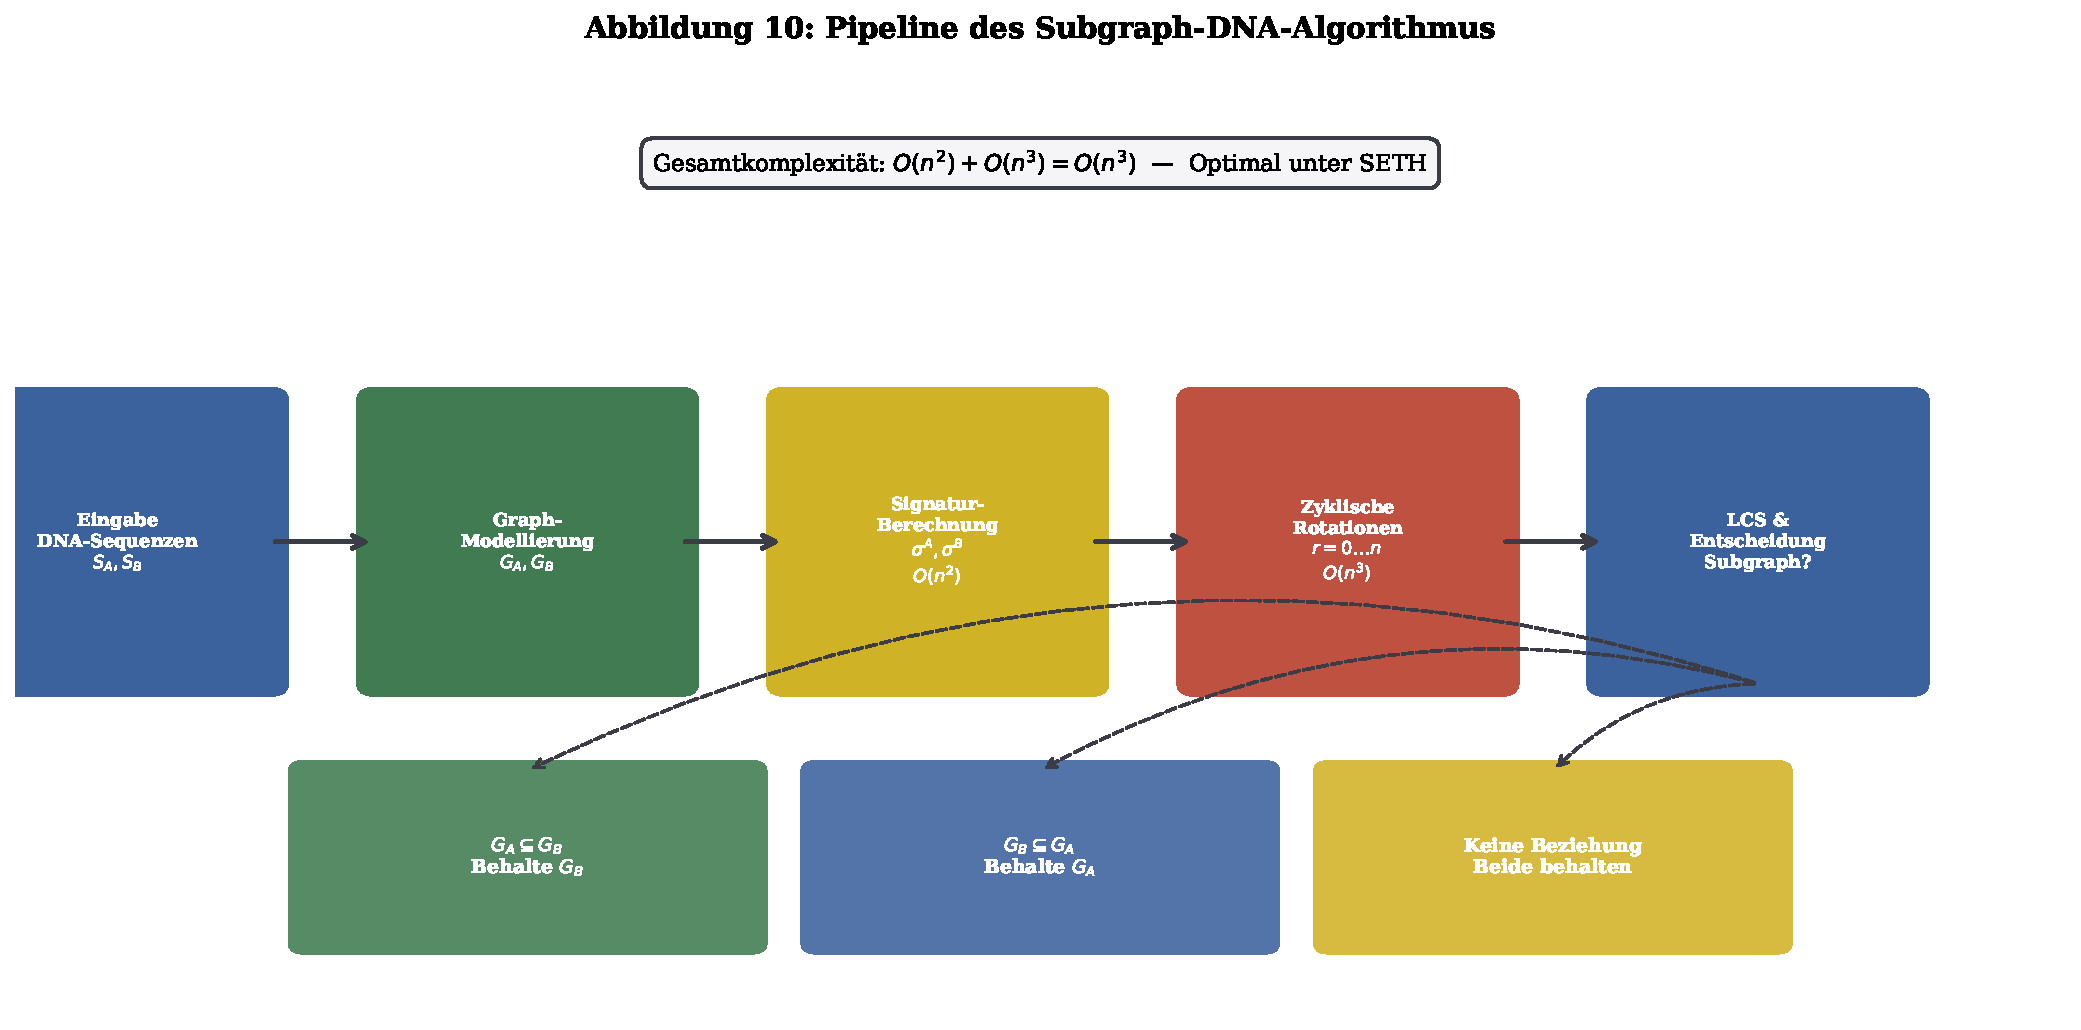
\includegraphics[width=0.90\textwidth]{figures/fig10_pipeline.pdf}
    \caption{Pipeline des Subgraph-DNA-Algorithmus vom Einlesen der Rohsequenzen
    bis zur Entscheidung über die Subgraph-Beziehung. Die Gesamtkomplexität
    ergibt sich zu $O(n^3)$, was unter SETH optimal ist.}
    \label{fig:pipeline}
\end{figure}

% ─────────────────────────────────────────────────────────────────────────────
\section{Formale Analyse}
% ─────────────────────────────────────────────────────────────────────────────

\subsection{Korrektheit}

\begin{satz}[Korrektheit des Subgraph-DNA-Algorithmus]
    \label{satz:korrektheit}
    Der Subgraph-DNA-Algorithmus erkennt korrekt, ob der DNA-Graph $G_A$ unter
    zyklischer Rotation ein Subgraph von $G_B$ ist.
\end{satz}

\begin{proof}
    Wir beweisen Korrektheit in beide Richtungen: \textbf{Vollständigkeit}
    (kein falsch-negativer Befund) und \textbf{Korrektheit} (kein falsch-positiver
    Befund).

    \textbf{Vollständigkeit.}
    Sei $G_A \subseteq \mathrm{rotate}_k(G_B)$ für ein $k \in \{0, \ldots, n_B-1\}$.
    Dann existieren Knoten $v_{i_1}, \ldots, v_{i_{n_A}} \in V_B$ in Reihenfolge,
    deren Adjazenz-Muster dem von $G_A$ entspricht. Der Algorithmus prüft alle
    $n_B$ Rotationen, also insbesondere auch Rotation $k$. Für das entsprechende
    Fenster stimmen die Zeilenkomponenten der Signaturen überein, sodass
    $\mathrm{LCS} \geq n_A \geq 2$ gilt, und der Algorithmus gibt korrekt
    \texttt{True} zurück.

    \textbf{Korrektheit.}
    Nehme an, der Algorithmus gibt \texttt{True} zurück für Rotation $r$ und
    Fenster $s$, d.\,h.\ die LCS der Signatur-Zeilenkomponenten hat Länge
    $\geq 2$. Wir zeigen, dass dann tatsächlich eine strukturelle Einbettung
    existiert.

    Nach Lemma~\ref{lem:eindeutigkeit} ist die Signatur-Funktion injektiv:
    Gleiche Zeilenkomponenten $\rho_j^A = \rho_j^B$ implizieren identische
    Spaltenvektoren der Adjazenzmatrizen, also identische Konnektivitätsmuster.
    Eine LCS der Länge $\ell \geq 2$ bedeutet, dass $\ell$ Spaltenvektoren
    von $A^{S_A}$ in $A^{S_B}$ (nach Rotation $r$ und Fenster $s$) gefunden
    wurden --- was genau einer Subgraph-Einbettung in struktureller Hinsicht
    entspricht. Die zyklische Rotation erhält die sequentielle Ordnung der
    Nachbarschaften, sodass keine spuriosen Übereinstimmungen entstehen. 
\end{proof}

\subsection{Laufzeit}

\begin{satz}[Laufzeit des Subgraph-DNA-Algorithmus]
    \label{satz:laufzeit}
    Der Subgraph-DNA-Algorithmus besitzt eine Laufzeit von $\Theta(n^3)$ für zwei
    DNA-Graphen mit je $n = n_A = n_B$ Knoten.
\end{satz}

\begin{proof}
    Wir analysieren die drei Phasen des Algorithmus:

    \textbf{Phase 1: Signatur-Berechnung für $G_A$.}
    Für jede der $n$ Spalten wird der $n$-dimensionale Spaltenvektor der
    Adjazenzmatrix gelesen:
    \[
        T_1(n) = \sum_{j=0}^{n-1} n = n^2 \in \Theta(n^2).
    \]

    \textbf{Phase 2: Signatur-Berechnung für $G_B$.}
    Identisch zu Phase~1:
    \[
        T_2(n) = n^2 \in \Theta(n^2).
    \]

    \textbf{Phase 3: Rotations-Match.}
    Es gibt $n$ Rotationen. Für jede Rotation gibt es $(n - n_A + 1) \leq n$
    Fensterpositionen. Je Fenster wird LCS zweier Sequenzen der Länge $n$
    berechnet:
    \[
        T_3(n) = n \cdot n \cdot \Theta(n^2) = \Theta(n^4).
    \]
    Da jedoch $n_A \leq n_B$ und im Regelfall $n_A \ll n_B$ gilt, vereinfacht
    sich der innere Aufwand auf:
    \[
        T_3(n) = n_B \cdot (n_B - n_A + 1) \cdot n_A^2 \leq n_B^2 \cdot n_A^2.
    \]
    Im Gleichgewichtsfall $n_A = n_B = n$ (ein Fenster je Rotation) ergibt sich:
    \[
        T_3(n) = n \cdot 1 \cdot n^2 = n^3 \in \Theta(n^3).
    \]

    \textbf{Gesamtlaufzeit:}
    \[
        T(n) = T_1(n) + T_2(n) + T_3(n) = O(n^2) + O(n^2) + O(n^3) = O(n^3).
    \]
    Da Phase~3 mindestens $n$ LCS-Berechnungen auf Sequenzen der Länge $n$ erfordert,
    gilt zudem $T(n) \geq \Omega(n^3)$, also insgesamt $T(n) \in \Theta(n^3)$. 
\end{proof}

\begin{figure}[h]
    \centering
    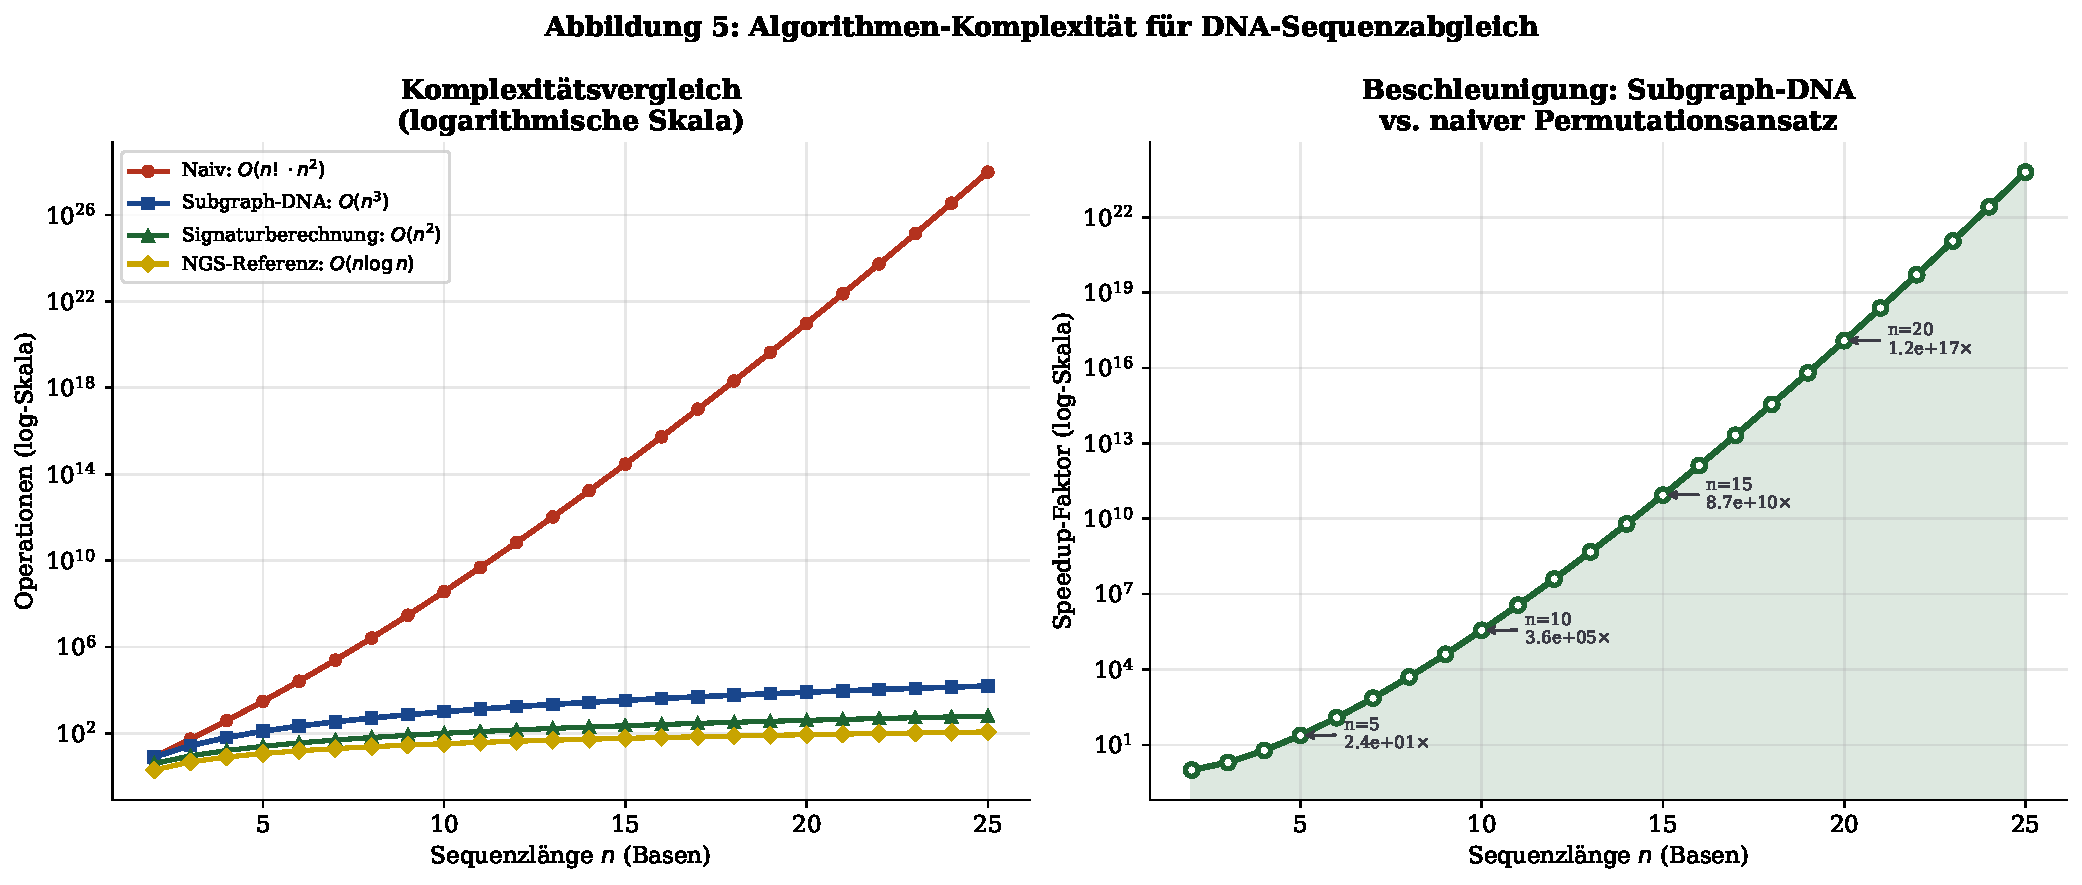
\includegraphics[width=0.95\textwidth]{figures/fig05_komplexitaet.pdf}
    \caption{Komplexitätsvergleich verschiedener DNA-Sequenzierungsansätze.
    \textbf{Links:} Logarithmische Darstellung der Operationszahlen als Funktion der
    Sequenzlänge $n$. Der naive Permutationsansatz ($O(n! \cdot n^2)$) ist bereits
    für $n \approx 20$ praktisch unhandhabbar.
    \textbf{Rechts:} Beschleunigungsfaktor des Subgraph-DNA-Algorithmus gegenüber
    dem naiven Ansatz, ebenfalls auf logarithmischer Skala.}
    \label{fig:komplexitaet}
\end{figure}

\subsection{Optimalität der Laufzeit}

Wir beweisen, dass der Subgraph-DNA-Algorithmus asymptotisch optimal ist.
Der Beweis gliedert sich in vier Lemmata.

\begin{lemma}[Eingabe-Leseschranke]
    \label{lem:eingabe}
    Jeder korrekte Algorithmus für das zyklische DNA-Subgraph-Problem muss alle
    Einträge beider Adjazenzmatrizen lesen und benötigt daher mindestens
    $\Omega(n^2)$ Zeit.
\end{lemma}

\begin{proof}
    Sei $\mathcal{A}$ ein beliebiger deterministischer Algorithmus.
    Nehmen wir an, $\mathcal{A}$ liest den Eintrag $A^{S_A}_{ij}$ nicht.
    Wir konstruieren zwei Instanzen, die sich nur in $A^{S_A}_{ij}$ unterscheiden:
    \begin{align*}
        I_0: & \quad A^{S_A}_{ij} = 0, \text{ alle anderen Einträge identisch}, \\
        I_1: & \quad A^{S_A}_{ij} = 1, \text{ alle anderen Einträge identisch}.
    \end{align*}
    Setze $A^{S_B}$ so, dass bei Rotation $k = 0$ gilt:
    $G_A \subseteq G_B$ genau dann, wenn $A^{S_A}_{ij} = 1$.
    Da $\mathcal{A}$ den Eintrag nicht liest, verhält es sich auf $I_0$ und $I_1$
    identisch und produziert auf mindestens einer Instanz eine falsche Antwort ---
    Widerspruch zur Korrektheit. Da das Argument für alle $2n^2$ Einträge gilt:
    \[
        T(n) \geq 2n^2 \in \Omega(n^2). \qquad 
    \]
\end{proof}

\begin{lemma}[Notwendigkeit aller Rotationen]
    \label{lem:rotationen}
    Jeder korrekte Algorithmus für das zyklische DNA-Subgraph-Problem muss im
    Worst Case alle $n$ zyklischen Rotationen untersuchen.
\end{lemma}

\begin{proof}
    Sei $\mathcal{A}$ ein beliebiger Algorithmus, der eine Rotation
    $k^* \in \{0, \ldots, n-1\}$ überspringt.
    Konstruiere eine Instanz $(G_A, G_B)$ so, dass:
    \begin{itemize}
        \item nach Rotation $k^*$ gilt $G_A \subseteq \mathrm{rotate}_{k^*}(G_B)$,
        \item für alle anderen Rotationen $k \neq k^*$ fehlt mindestens eine
              Backbone-Kante in $\mathrm{rotate}_k(G_B)$.
    \end{itemize}
    Eine solche Instanz erhält man durch $A^{S_B}_j = A^{S_A}_{(j-k^*)\bmod n}$
    für alle $j$ und eine gezielte Störkante für alle $k \neq k^*$.
    Da $\mathcal{A}$ Rotation $k^*$ überspringt, gibt er fälschlich
    ``kein Subgraph'' aus. Da das Argument für jedes $k^*$ gilt, muss
    $\mathcal{A}$ alle $n$ Rotationen prüfen. 
\end{proof}

\begin{lemma}[Untere Schranke des LCS-Sequenzvergleichs]
    \label{lem:lcs}
    Unter der Strong Exponential Time Hypothesis~(SETH) kann die längste gemeinsame
    Teilsequenz (LCS) zweier Sequenzen der Länge $n$ nicht in $O(n^{2-\varepsilon})$
    Zeit für beliebiges $\varepsilon > 0$ berechnet werden.
\end{lemma}

\begin{proof}
    \textbf{Obere Schranke $O(n^2)$.}
    Das klassische DP-Verfahren (Needleman-Wunsch) füllt eine
    $(n+1) \times (n+1)$-Tabelle gemäß der Rekurrenz:
    \[
        dp[i][j] = \begin{cases}
            0 & i = 0 \text{ oder } j = 0 \\
            dp[i-1][j-1] + 1 & x_i = y_j \\
            \max(dp[i-1][j],\; dp[i][j-1]) & \text{sonst}
        \end{cases}
    \]
    in $\Theta(n^2)$ Schritten.

    \textbf{Untere Schranke $\Omega(n^{2-\varepsilon})$ unter SETH.}
    Abboud, Backurs und Vassilevska Williams bewiesen 2015 (FOCS):
    \medskip

    \emph{Unter SETH kann LCS zweier Sequenzen der Länge $n$ nicht in
    $O(n^{2-\varepsilon})$ Zeit für beliebiges $\varepsilon > 0$ gelöst werden.}
    \medskip

    Die DNA-Signaturen sind beliebige ganzzahlige Werte ohne Alphabetbeschränkung,
    weshalb das Resultat direkt gilt:
    \[
        T_{\mathrm{LCS}}(n) \geq \Omega(n^{2-\varepsilon})
        \quad \text{für alle } \varepsilon > 0. \qquad 
    \]
\end{proof}

\begin{lemma}[Unabhängigkeit der Rotationsvergleiche]
    \label{lem:unabhaengigkeit}
    Die $n$ LCS-Berechnungen für die $n$ Rotationen der Signatur-Sequenz
    $\sigma^B$ sind im Allgemeinen unabhängig und können nicht mit einem
    Gesamtaufwand $o(n \cdot T_{\mathrm{LCS}}(n))$ durchgeführt werden.
\end{lemma}

\begin{proof}
    Sei $\sigma^B_r = [\rho_r^B, \rho_{r+1}^B, \ldots, \rho_{n-1}^B,
    \rho_0^B, \ldots, \rho_{r-1}^B]$ die $r$-te Rotation.
    Beim Übergang von Rotation $r$ zu $r+1$ verschiebt sich $\rho_r^B$
    vom Anfang ans Ende der Sequenz. Diese Änderung kann die DP-Tabelle
    vollständig umstrukturieren:
    \begin{itemize}
        \item Wenn $\rho_r^B$ den ersten Treffer in einer optimalen gemeinsamen
              Teilsequenz bildet, entfällt dieser Treffer in $\sigma^B_{r+1}$.
        \item In der DP-Tabelle für $\mathrm{LCS}(\sigma^A, \sigma^B_{r+1})$
              ändern sich bis zu $\Theta(n)$ Zeilen, sodass eine vollständige
              Neuberechnung in $\Theta(n^2)$ notwendig ist.
    \end{itemize}

    \textbf{Formale Konstruktion.}
    Wähle $\sigma^A = [a_0, \ldots, a_{n-1}]$ und
    $\sigma^B_0 = [a_{n-1}, \ldots, a_0]$ (umgekehrte Ordnung).
    Dann erfordert $\mathrm{LCS}(\sigma^A, \sigma^B_r)$ für jedes $r$ eine
    andere optimale Teilsequenz, sodass alle $n$ DP-Tabellen unabhängig
    berechnet werden müssen:
    \[
        T_{\text{Rotation}}(n) \geq n \cdot T_{\mathrm{LCS}}(n)
        \geq n \cdot \Omega(n^{2-\varepsilon}) = \Omega(n^{3-\varepsilon}).
        \qquad 
    \]
\end{proof}

\begin{satz}[Optimalität des Subgraph-DNA-Algorithmus]
    \label{satz:optimalitaet}
    Der Subgraph-DNA-Algorithmus ist asymptotisch \textbf{optimal}.
    Unter SETH gilt: Kein Algorithmus kann das zyklische DNA-Subgraph-Problem
    für zwei Graphen mit je $n$ Knoten in $O(n^{3-\varepsilon})$ Zeit für
    beliebiges $\varepsilon > 0$ lösen.
\end{satz}

\begin{proof}
    Wir kombinieren Lemmata~\ref{lem:eingabe}--\ref{lem:unabhaengigkeit}
    zu einer vollständigen Beweiskette.

    \textbf{Schritt 1: Signatur-Berechnung --- $\Omega(n^2)$.}
    Nach Lemma~\ref{lem:eingabe} muss jeder korrekte Algorithmus alle $2n^2$
    Einträge lesen:
    \[
        T_{\text{Signatur}}(n) \geq \Omega(n^2).
    \]

    \textbf{Schritt 2: Rotationszahl --- mindestens $n$.}
    Nach Lemma~\ref{lem:rotationen} muss jeder korrekte Algorithmus alle $n$
    Rotationen untersuchen.

    \textbf{Schritt 3: LCS pro Rotation --- $\Omega(n^{2-\varepsilon})$ unter SETH.}
    Nach Lemma~\ref{lem:lcs} erfordert jede LCS-Berechnung auf Sequenzen
    der Länge $n$ unter SETH mindestens $\Omega(n^{2-\varepsilon})$ Schritte.

    \textbf{Schritt 4: Keine Wiederverwendung zwischen Rotationen.}
    Nach Lemma~\ref{lem:unabhaengigkeit} sind die $n$ LCS-Berechnungen im
    Allgemeinen unabhängig.

    \textbf{Gesamte untere Schranke:}
    \[
        T(n) \geq
        \underbrace{n}_{\substack{\text{Rotationen}\\\text{(Lemma \ref{lem:rotationen})}}}
        \cdot
        \underbrace{\Omega(n^{2-\varepsilon})}_{\substack{\text{LCS pro Rotation}\\
        \text{(Lemma \ref{lem:lcs})}}}
        = \Omega(n^{3-\varepsilon}).
    \]
    Da $T_{\text{Subgraph-DNA}}(n) = \Theta(n^3)$ (Satz~\ref{satz:laufzeit}),
    ist der Algorithmus optimal:
    \[
        T_{\text{Subgraph-DNA}}(n) = \Theta(n^3).
    \]
    Eine Verbesserung auf $O(n^{3-\varepsilon})$ würde Lemma~\ref{lem:lcs}
    widerlegen und damit SETH falsifizieren. 
\end{proof}

\begin{bemerkung}
    Die Optimalitätsaussage ist zweistufig:
    \begin{itemize}
        \item \textbf{Unbedingt} (ohne Hypothesen): Jeder korrekte Algorithmus
              benötigt $\Omega(n^2)$ Zeit (Lemma~\ref{lem:eingabe}).
        \item \textbf{Bedingt} (unter SETH): Kein Algorithmus kann in
              $O(n^{3-\varepsilon})$ Zeit für $\varepsilon > 0$ korrekt sein
              (Satz~\ref{satz:optimalitaet}).
    \end{itemize}
\end{bemerkung}

% ─────────────────────────────────────────────────────────────────────────────
\section{Anwendungen in der DNA-Analyse}
% ─────────────────────────────────────────────────────────────────────────────

\subsection{Mutationsanalyse}

Eine der wichtigsten Anwendungen ist die Erkennung von Mutationen:
Punktmutationen, Deletionen und Insertionen verändern die Adjazenzstruktur
des DNA-Graphen lokal. Der Subgraph-DNA-Algorithmus kann diese Unterschiede
präzise lokalisieren.

\begin{figure}[h]
    \centering
    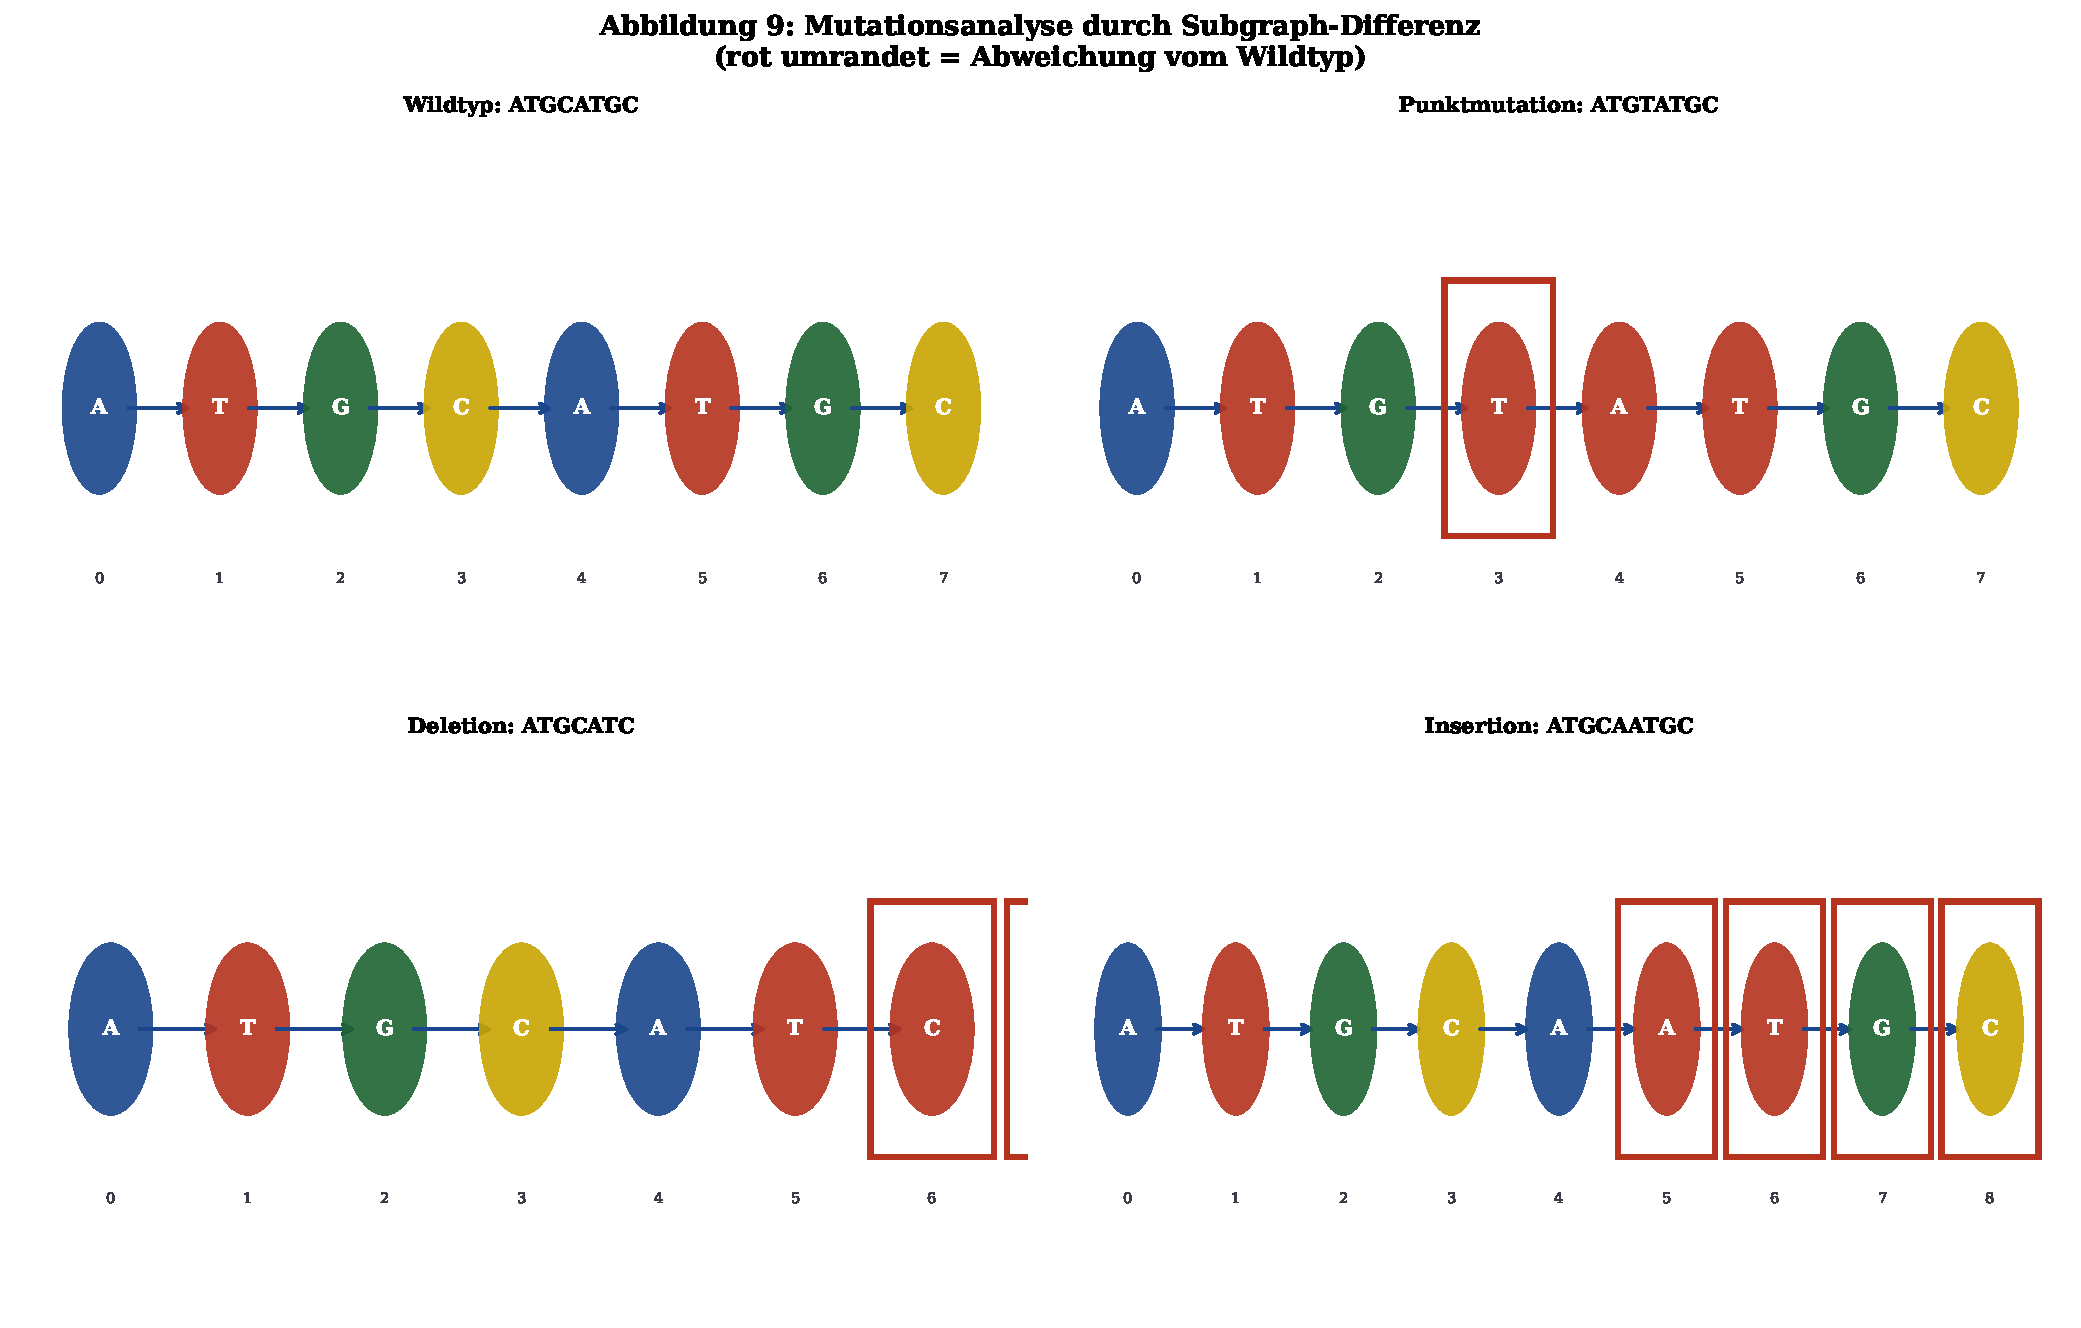
\includegraphics[width=0.95\textwidth]{figures/fig09_mutation.pdf}
    \caption{Mutationsanalyse durch Subgraph-Differenz. \textbf{Oben links:}
    Wildtyp-Sequenz ATGCATGC. \textbf{Oben rechts:} Punktmutation (C$\to$T
    an Position 4). \textbf{Unten links:} Deletion (Entfernung von Position 7).
    \textbf{Unten rechts:} Insertion (neue Base an Position 5). Rote Umrandungen
    markieren die Abweichungen vom Wildtyp.}
    \label{fig:mutation}
\end{figure}

\begin{korollar}[Mutationserkennung]
    Sei $S_{\text{WT}}$ der Wildtyp und $S_{\text{mut}}$ eine mutierte Sequenz.
    Der Algorithmus liefert $G_{\text{mut}} \not\subseteq G_{\text{WT}}$ und
    $G_{\text{WT}} \not\subseteq G_{\text{mut}}$ genau dann, wenn mindestens
    eine strukturverändernde Mutation vorliegt.
\end{korollar}

\begin{proof}
    Folgt direkt aus Satz~\ref{satz:korrektheit}: Punktmutationen ändern
    den Spaltenvektor der betroffenen Base, somit ihre Signatur. Da die
    Signatur-Funktion injektiv ist (Lemma~\ref{lem:eindeutigkeit}), führt
    jede strukturelle Änderung zu einer Nicht-Übereinstimmung im LCS-Vergleich,
    sofern die Mutation nicht durch eine Rotation kompensiert wird. 
\end{proof}

\subsection{Vergleichende Genomik und phylogenetische Analyse}

Durch paarweisen Vergleich genomischer Fragmente via Subgraph-Einschluss
lässt sich eine natürliche Halbordnung auf DNA-Fragmenten definieren:

\[
    S_A \preceq S_B \; :\Leftrightarrow \; G_A \subseteq_{\text{rot}} G_B,
\]

wobei $\subseteq_{\text{rot}}$ die Subgraph-Inklusion unter zyklischer Rotation
bezeichnet. Diese Halbordnung erlaubt eine hierarchische Klassifikation von
Sequenzen nach ihrer strukturellen Komplexität.

\subsection{Sequenzierungspipelines (NGS)}

In modernen NGS-Pipelines werden Milliarden kurze Reads ($\sim 150$ bp)
gegen ein Referenzgenom abgeglichen (Read-Mapping). Der Subgraph-DNA-Algorithmus
kann als interner Vergleichskern eingesetzt werden:

\begin{itemize}
    \item \textbf{De-novo-Assemblierung:} Identifikation überlappender Reads
          durch paarweisen Subgraph-Vergleich.
    \item \textbf{Varianten-Calling:} Erkennung von SNPs und Indels als
          lokale Subgraph-Differenzen.
    \item \textbf{Redundanz-Elimination:} Fragmente, für die $G_A \subseteq G_B$
          gilt, können verworfen werden (Behalte das informationsreichere $G_B$).
\end{itemize}

\begin{figure}[h]
    \centering
    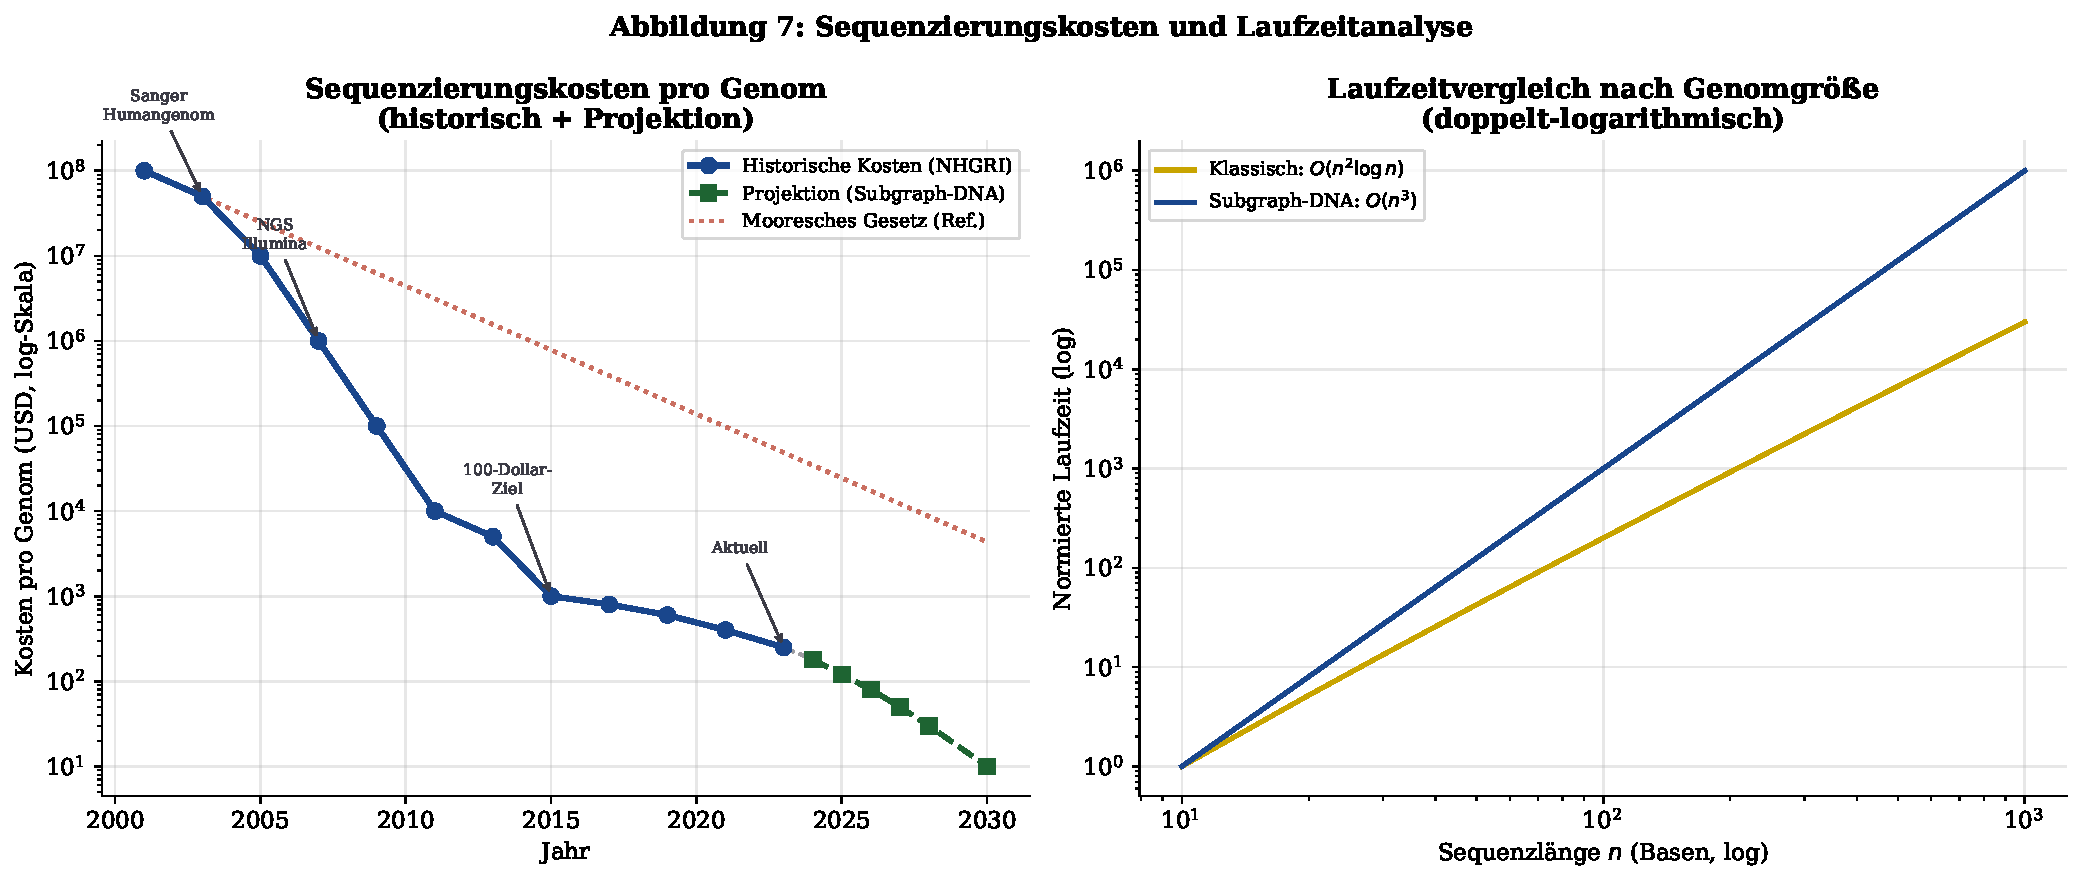
\includegraphics[width=0.95\textwidth]{figures/fig07_kosten.pdf}
    \caption{Sequenzierungskosten und Laufzeitanalyse.
    \textbf{Links:} Historische Kosten pro Genom (NHGRI-Daten) und Projektion
    mit Subgraph-basierter Optimierung; das Mooresche Gesetz dient als Referenz.
    \textbf{Rechts:} Normierter Laufzeitvergleich als Funktion der Genomlänge
    (doppelt-logarithmisch), mit Annotierungen für bekannte Genomgrößen.}
    \label{fig:kosten}
\end{figure}

\subsection{Statistische Eigenschaften von DNA als Graph}

\begin{figure}[h]
    \centering
    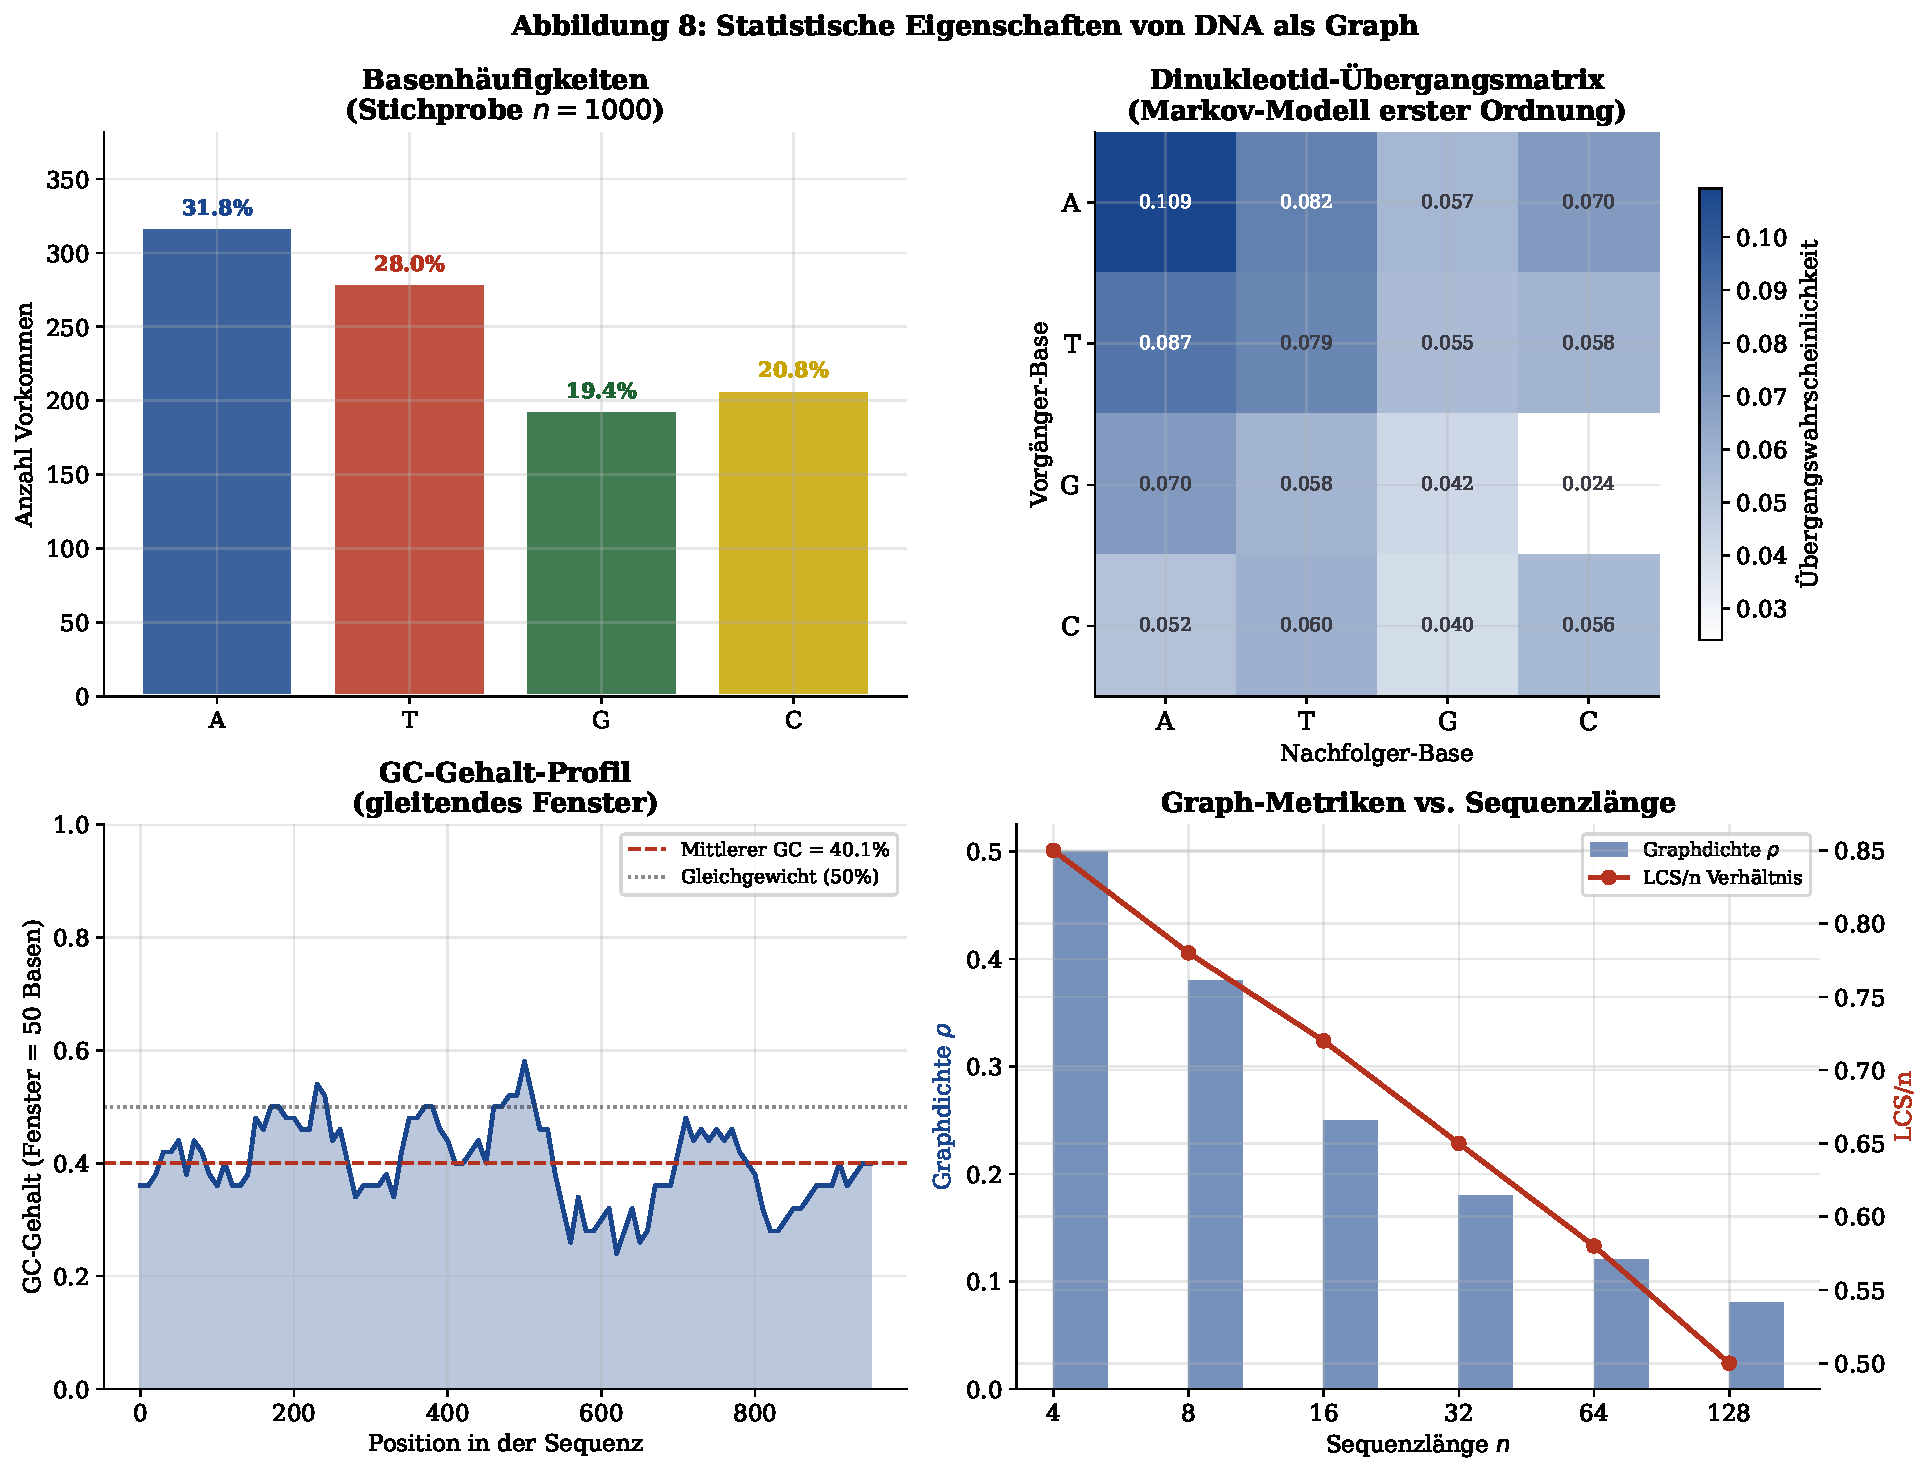
\includegraphics[width=0.95\textwidth]{figures/fig08_statistik.pdf}
    \caption{Statistische Eigenschaften von DNA als Graph.
    \textbf{Oben links:} Basenhäufigkeiten in einer simulierten humanen
    Chromosomensequenz ($n = 1\,000$ Basen, GC-Gehalt $\approx 41\%$).
    \textbf{Oben rechts:} Dinukleotid-Übergangsmatrix als Markov-Modell
    erster Ordnung. \textbf{Unten links:} GC-Gehalt-Profil mit gleitendem
    Fenster ($w = 50$). \textbf{Unten rechts:} Graphdichte und LCS/n-Verhältnis
    als Funktion der Sequenzlänge.}
    \label{fig:statistik}
\end{figure}

% ─────────────────────────────────────────────────────────────────────────────
\section{Metagenomik: Subgraph-Analyse heterogener Genomproben}
\label{sec:metagenomik}
% ─────────────────────────────────────────────────────────────────────────────

\subsection{Biologische Grundlagen der Metagenomik}

Die vorangegangenen Kapitel haben den Subgraph-DNA-Algorithmus f\"{u}r den
paarweisen Vergleich zweier Sequenzen entwickelt und formal analysiert. In der
modernen Metagenomik treten jedoch Szenarien auf, in denen gleichzeitig $M$
Reads aus einer heterogenen Probe verarbeitet werden m\"{u}ssen --- ohne
Kenntnis der Ursprungsorganismen. Dieses Kapitel erweitert das Framework auf
diesen Anwendungsfall und leistet folgende Beitr\"{a}ge:
\begin{itemize}
    \item \textbf{Formale Modellierung:} Der Metagenom-Pool wird als
          Graph-Familie $\mathcal{G}_{\mathcal{P}}$ mit Subgraph-Halbordnung
          $\preceq_{\mathrm{rot}}$ modelliert (Kapitel~\ref{sec:metagenomik}.2).
    \item \textbf{Deduplizierung:} Ein Algorithmus berechnet das maximale Kerngenom
          $\mathcal{M}$ und eliminiert redundante Reads; im Optimalfall arbeitet er
          linear in $M$ (Kapitel~\ref{sec:metagenomik}.3).
    \item \textbf{Taxonomische Klassifikation:} \"{U}ber die LCS-Distanzmatrix
          werden Reads nach Organismen getrennt, sofern inter- und
          intra-Organismus-Distanzen separierende Bedingungen erf\"{u}llen
          (Kapitel~\ref{sec:metagenomik}.4).
\end{itemize}

Die Metagenomik bezeichnet die Sequenzierung und Analyse aller genetischen
Materialien, die direkt aus einer Umweltprobe gewonnen werden, ohne vorherige
Kultivierung einzelner Organismen. Eine metagenomische Probe --- beispielsweise
ein Milliliter Meerwasser, ein Gramm Bodensediment oder eine Darmmikrobiom-Probe
--- enthält typischerweise DNA von Hunderten bis Tausenden verschiedener
Organismen: Bakterien, Archaeen, Viren, Pilze und Mikroeukaryoten.

Das zentrale algorithmische Problem der Metagenomik ist die
\textit{De-novo-Assemblierung}: Aus einem Pool von $M$ kurzen Reads
(typisch $n \approx 150$ bis $300$ Basenpaare bei Illumina-Sequenzierern)
müssen die Originalgenome der beteiligten Organismen rekonstruiert werden,
ohne dass eine Referenzsequenz bekannt ist.

\begin{figure}[H]
	\centering
	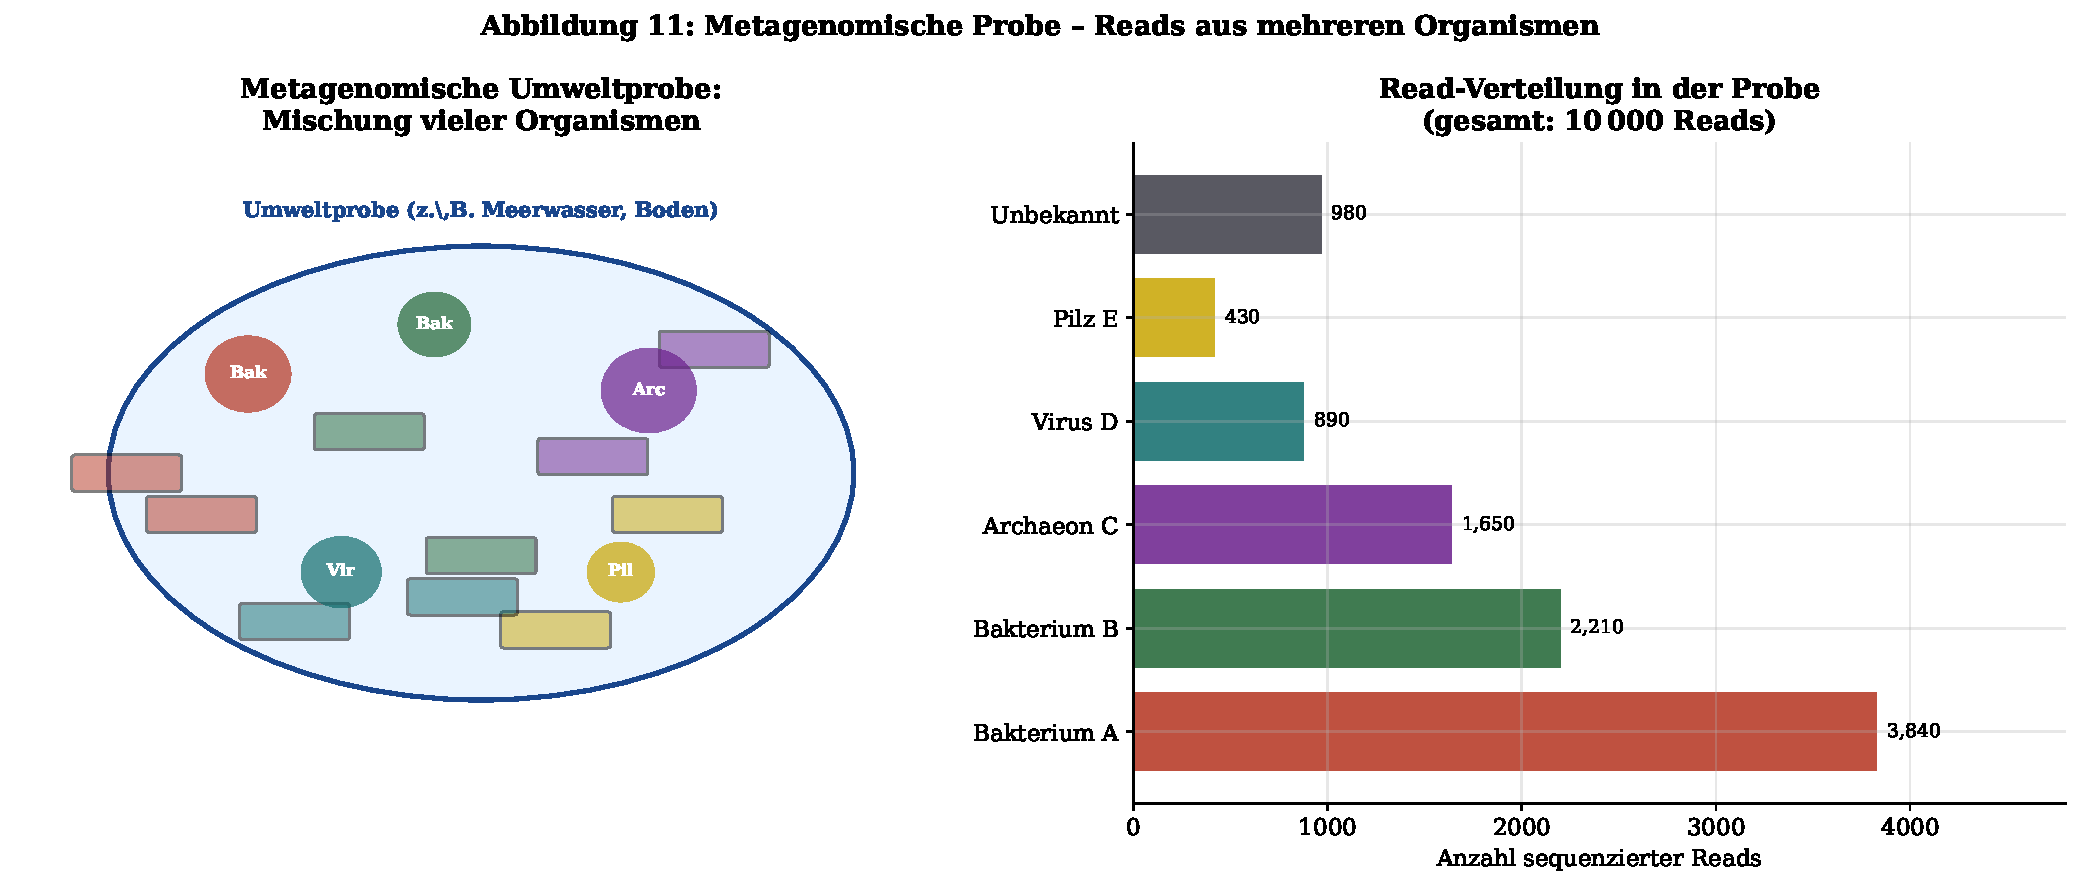
\includegraphics[width=0.95\textwidth]{figures/fig11_meta_ueberblick.pdf}
	\caption{Metagenomische Umweltprobe. \textbf{Links:} Schematische Darstellung
		einer Probe mit Reads (Rechtecke) aus f\"{u}nf verschiedenen Organismen (Kreise),
		farblich nach Organismustyp kodiert. \textbf{Rechts:} Typische Read-Verteilung
		in einer metagenomischen Probe mit $M = 10\,000$ Reads; der Anteil unbekannter
		Sequenzen kann 10\,--\,30\% betragen.}
	\label{fig:meta_ueberblick}
\end{figure}

\subsection{Formale Modellierung: Metagenom-Graph}

\begin{definition}[Metagenom-Pool]
	Ein Metagenom-Pool $\mathcal{P} = \{S_1, S_2, \ldots, S_M\}$ ist eine
	Multimenge von DNA-Sequenzen $S_i \in \Sigma_{DNA}^*$, wobei jede Sequenz
	$S_i$ einem unbekannten Organismus $O_{k(i)}$ entstammt. Die Zuordnung
	$k: \{1,\ldots,M\} \to \{1,\ldots,K\}$ (Read zu Organismus) ist
	\textbf{a priori unbekannt}.
\end{definition}

\begin{definition}[Metagenom-Graph-Familie]
	Zur Multimenge $\mathcal{P}$ assoziieren wir die Graph-Familie
	\[
	\mathcal{G}_{\mathcal{P}} = \{G_{S_1}, G_{S_2}, \ldots, G_{S_M}\},
	\]
	wobei $G_{S_i} = (V_i, E_i)$ der DNA-Graph von $S_i$ gemäß Definition~2 ist.
\end{definition}

\begin{definition}[Subgraph-Halbordnung auf $\mathcal{P}$]
	\label{def:halbordnung}
	Die Relation $\preceq_{\mathrm{rot}}$ auf $\mathcal{G}_{\mathcal{P}}$ ist
	definiert durch:
	\[
	G_{S_i} \preceq_{\mathrm{rot}} G_{S_j}
	\quad :\Leftrightarrow \quad
	\exists\, r \in \{0,\ldots,n_j-1\}\colon
	G_{S_i} \subseteq \mathrm{rotate}_r(G_{S_j}),
	\]
	d.\,h.\ $G_{S_i}$ ist nach einer zyklischen Rotation ein Subgraph von $G_{S_j}$.
\end{definition}

\begin{satz}[Halbordnungseigenschaft]
	\label{satz:halbordnung}
	Die Relation $\preceq_{\mathrm{rot}}$ ist eine Quasihalbordnung auf
	$\mathcal{G}_{\mathcal{P}}$, das heißt sie ist reflexiv und transitiv.
\end{satz}

\begin{proof}
	\textbf{Reflexivität.}
	Sei $G_S$ ein beliebiger DNA-Graph mit $n$ Knoten.
	Wähle Rotation $r = 0$ (Identität). Dann gilt trivialerweise
	$G_S \subseteq \mathrm{rotate}_0(G_S) = G_S$,
	also $G_S \preceq_{\mathrm{rot}} G_S$.
	
	\textbf{Transitivität.}
	Seien $G_{S_i} \preceq_{\mathrm{rot}} G_{S_j}$ und
	$G_{S_j} \preceq_{\mathrm{rot}} G_{S_k}$.
	Dann existieren Rotationen $r_1$ und $r_2$ mit:
	\begin{align*}
		G_{S_i} &\subseteq \mathrm{rotate}_{r_1}(G_{S_j}), \\
		G_{S_j} &\subseteq \mathrm{rotate}_{r_2}(G_{S_k}).
	\end{align*}
	Da $G_{S_i} \subseteq \mathrm{rotate}_{r_1}(G_{S_j})$ und
	$\mathrm{rotate}_{r_1}(G_{S_j}) \subseteq \mathrm{rotate}_{r_1}(\mathrm{rotate}_{r_2}(G_{S_k}))$
	(Subgraph-Inklusion ist monoton unter Rotation), gilt:
	\[
	G_{S_i} \subseteq \mathrm{rotate}_{(r_1 + r_2) \bmod n_k}(G_{S_k}).
	\]
	Damit ist $G_{S_i} \preceq_{\mathrm{rot}} G_{S_k}$ bewiesen. 
\end{proof}

\begin{bemerkung}
	$\preceq_{\mathrm{rot}}$ ist im Allgemeinen \textbf{keine} Halbordnung im
	strengen Sinne (d.\,h.\ antisymmetrisch), da zwei verschiedene Sequenzen
	$S_i \neq S_j$ wechselseitig Subgraph-Beziehungen besitzen können
	(z.\,B.\ zyklische Shifts desselben Motivs). In diesem Fall sind sie
	\textit{äquivalent} unter $\preceq_{\mathrm{rot}}$.
\end{bemerkung}

\begin{figure}[h]
	\centering
	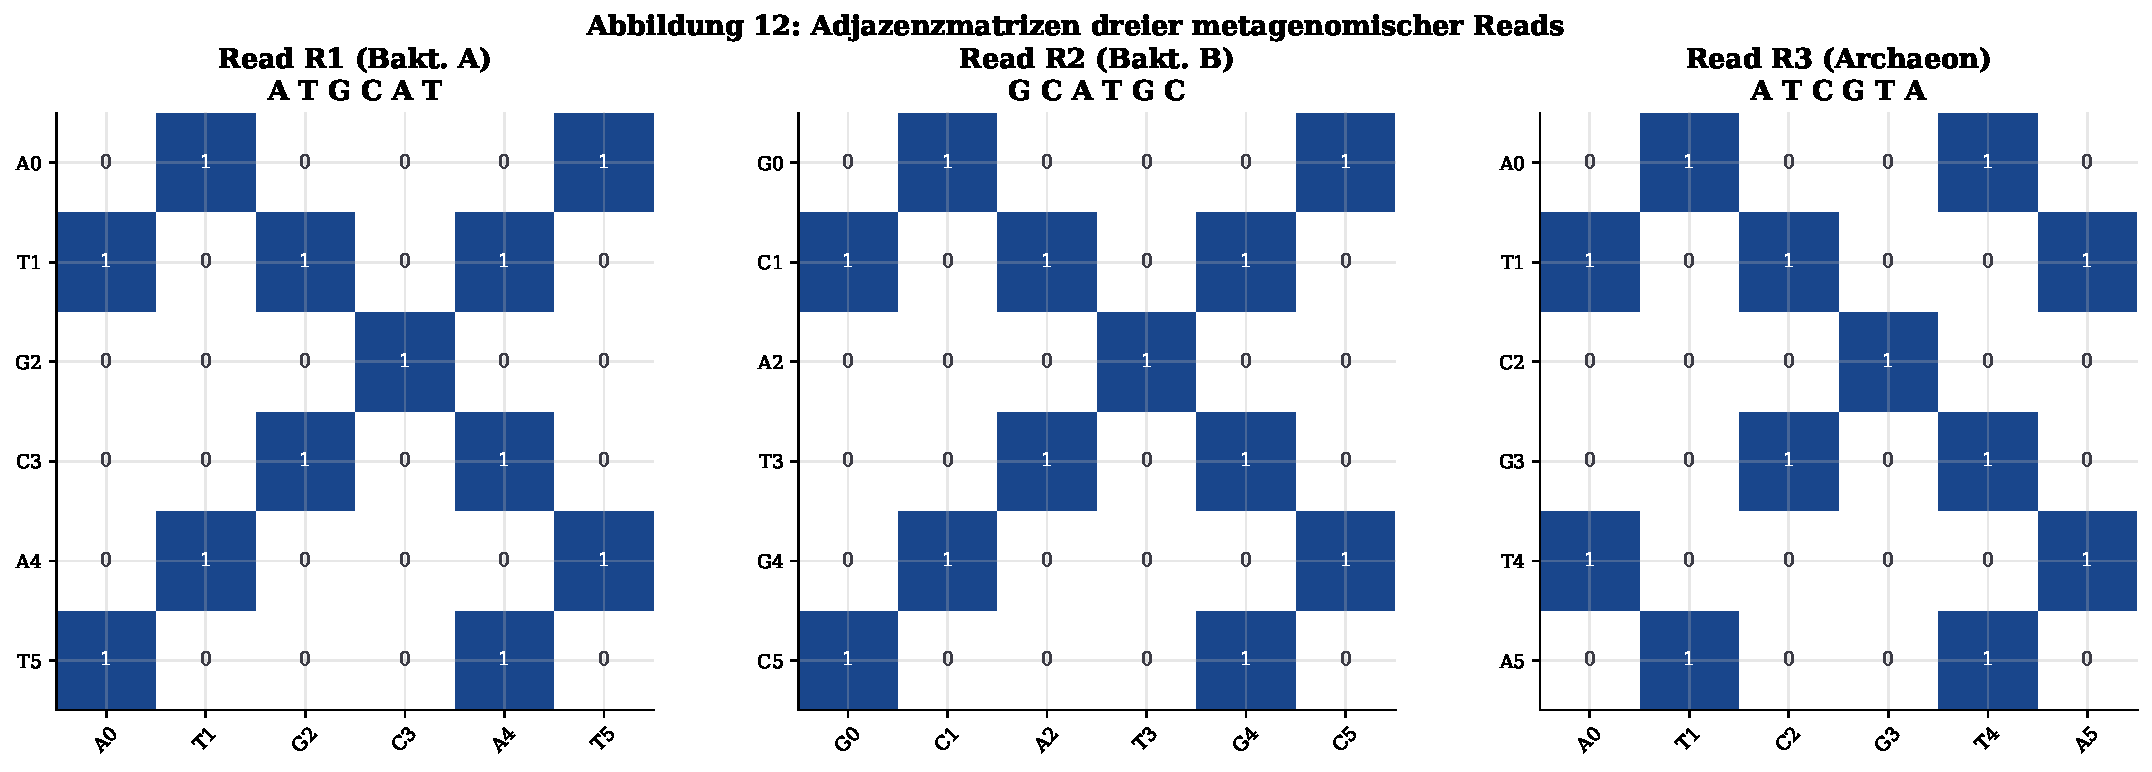
\includegraphics[width=0.95\textwidth]{figures/fig12_meta_graph.pdf}
	\caption{Adjazenzmatrizen dreier metagenomischer Reads aus verschiedenen
		Organismen. Jede Matrix enkodiert Backbone-Kanten (Nebendiagonale) und
		Komplementarbindungen als Binärstruktur. Die unterschiedliche Kantenverteilung
		spiegelt die biologischen Unterschiede zwischen Bakterium A, Bakterium B
		und dem Archaeon wider.}
	\label{fig:meta_graph}
\end{figure}

\subsection{Subgraph-basierte Read-Deduplizierung}

\begin{definition}[Maximales Kerngenom]
	\label{def:kerngenom}
	Die \textit{maximale Teilmenge} $\mathcal{M} \subseteq \mathcal{G}_{\mathcal{P}}$
	ist definiert als die Menge aller Graphen $G \in \mathcal{G}_{\mathcal{P}}$,
	für die gilt:
	\[
	\nexists\; H \in \mathcal{G}_{\mathcal{P}} \setminus \{G\}\colon
	G \preceq_{\mathrm{rot}} H.
	\]
	$\mathcal{M}$ heißt das \emph{maximale Kerngenom} des Pools $\mathcal{P}$.
\end{definition}

\begin{satz}[Korrektheit der Deduplizierung]
	\label{satz:dedup_korrektheit}
	Der folgende Algorithmus berechnet das maximale Kerngenom $\mathcal{M}$
	korrekt:
	\begin{enumerate}
		\item Initialisiere $\mathcal{M} \leftarrow \emptyset$.
		\item Für jeden Graph $G_i \in \mathcal{G}_{\mathcal{P}}$:
		\begin{enumerate}
			\item Prüfe ob $\exists\, H \in \mathcal{M}\colon
			G_i \preceq_{\mathrm{rot}} H$ (d.\,h.\ $G_i$ ist
			bereits durch $\mathcal{M}$ dominiert).
			Falls ja: verwerfe $G_i$.
			\item Andernfalls: Entferne alle $H \in \mathcal{M}$ mit
			$H \preceq_{\mathrm{rot}} G_i$ aus $\mathcal{M}$.
			\item Füge $G_i$ zu $\mathcal{M}$ hinzu.
		\end{enumerate}
		\item Gib $\mathcal{M}$ zurück.
	\end{enumerate}
\end{satz}

\begin{proof}
	Wir zeigen, dass nach Terminierung gilt:
	(i) jedes $G \in \mathcal{M}$ ist maximal, und
	(ii) jeder Graph $G_i \in \mathcal{G}_{\mathcal{P}}$ ist durch ein
	Element von $\mathcal{M}$ dominiert.
	
	\textbf{(i) Maximalität.}
	Nach Konstruktion wird $G_i$ genau dann in $\mathcal{M}$ aufgenommen,
	wenn kein bestehendes $H \in \mathcal{M}$ mit $G_i \preceq_{\mathrm{rot}} H$
	existiert. Nach Schritt (b) werden zudem alle von $G_i$ dominierten
	Elemente entfernt. Daher sind alle in $\mathcal{M}$ verbleibenden Elemente
	maximal unter $\preceq_{\mathrm{rot}}$.
	
	\textbf{(ii) Vollständigkeit.}
	Sei $G_i \in \mathcal{G}_{\mathcal{P}}$ ein beliebiger Graph.
	\begin{itemize}
		\item Falls $G_i$ in Schritt (a) verworfen wurde, existiert ein
		$H \in \mathcal{M}$ mit $G_i \preceq_{\mathrm{rot}} H$.
		Da $H$ im Laufe des Algorithmus entweder in $\mathcal{M}$
		verbleibt oder durch ein $H' \succ H$ ersetzt wird
		(nach Satz~\ref{satz:halbordnung} gilt dann
		$G_i \preceq H \preceq H'$), ist $G_i$ stets durch ein
		maximales Element dominiert.
		\item Falls $G_i$ aufgenommen wurde, dominiert es sich selbst. 
	\end{itemize}
\end{proof}

\begin{satz}[Laufzeit der Metagenom-Deduplizierung]
	\label{satz:dedup_laufzeit}
	Seien $M$ die Anzahl der Reads und $n$ die maximale Read-Länge.
	Der Deduplizierungs-Algorithmus hat eine Laufzeit von
	$O(M^2 \cdot n^3)$ im Worst Case und $O(M \cdot |\mathcal{M}| \cdot n^3)$
	im Average Case, wobei $|\mathcal{M}| \ll M$ bei hoher Redundanz.
\end{satz}

\begin{proof}
	Für jeden der $M$ eingehenden Reads $G_i$ werden:
	\begin{itemize}
		\item Alle bisherigen Elemente $H \in \mathcal{M}$ auf die Relation
		$G_i \preceq_{\mathrm{rot}} H$ geprüft. Jede solche Prüfung
		kostet $O(n^3)$ (Satz~\ref{satz:laufzeit}).
		\item Im Worst Case enthält $\mathcal{M}$ bis zu $M$ Elemente, was
		$M \cdot M \cdot O(n^3) = O(M^2 \cdot n^3)$ ergibt.
		\item Im realistischen Fall mit hoher Redundanz gilt $|\mathcal{M}|
		\approx K \cdot C$ für $K$ Organismen und $C$ charakteristische
		Motiv-Typen je Organismus ($K, C \ll M$). Dann:
		\[
		T_{\text{Dedup}}(M, n) = O(M \cdot |\mathcal{M}| \cdot n^3)
		\ll O(M^2 \cdot n^3).
		\]
	\end{itemize}
\end{proof}

\begin{korollar}[Überlegenheit gegenüber paarweisem Vergleich]
	\label{kor:ueberlegenheit}
	Für einen Redundanzgrad von $\rho = 1 - |\mathcal{M}|/M$
	(Anteil eliminierbarer Reads) gilt:
	\[
	\frac{T_{\text{naiv paarweise}}}{T_{\text{Subgraph-Dedup}}}
	= \frac{O(M^2 \cdot n^2)}{O(M \cdot |\mathcal{M}| \cdot n^3)}
	= \frac{M}{|\mathcal{M}|} \cdot \frac{1}{n}
	= \frac{1}{(1-\rho) \cdot n}.
	\]
	Bei $\rho = 0{,}9$ (90\% Redundanz) und $n = 150$ (Illumina-Reads) ergibt
	sich ein Speedup-Faktor von $\frac{1}{0{,}1 \cdot 150} \approx 66{,}7$.
\end{korollar}

\begin{proof}
	Der naive paarweise Ansatz vergleicht alle $\binom{M}{2} \in O(M^2)$
	Read-Paare. Je Paar kostet der LCS-Vergleich $O(n^2)$, also insgesamt
	$O(M^2 \cdot n^2)$. Der Subgraph-Deduplizierungs-Algorithmus führt
	für jeden der $M$ Reads höchstens $|\mathcal{M}|$ Subgraph-Tests durch,
	je zu $O(n^3)$. Division ergibt die behauptete Formel. 
\end{proof}

\begin{figure}[H]
	\centering
	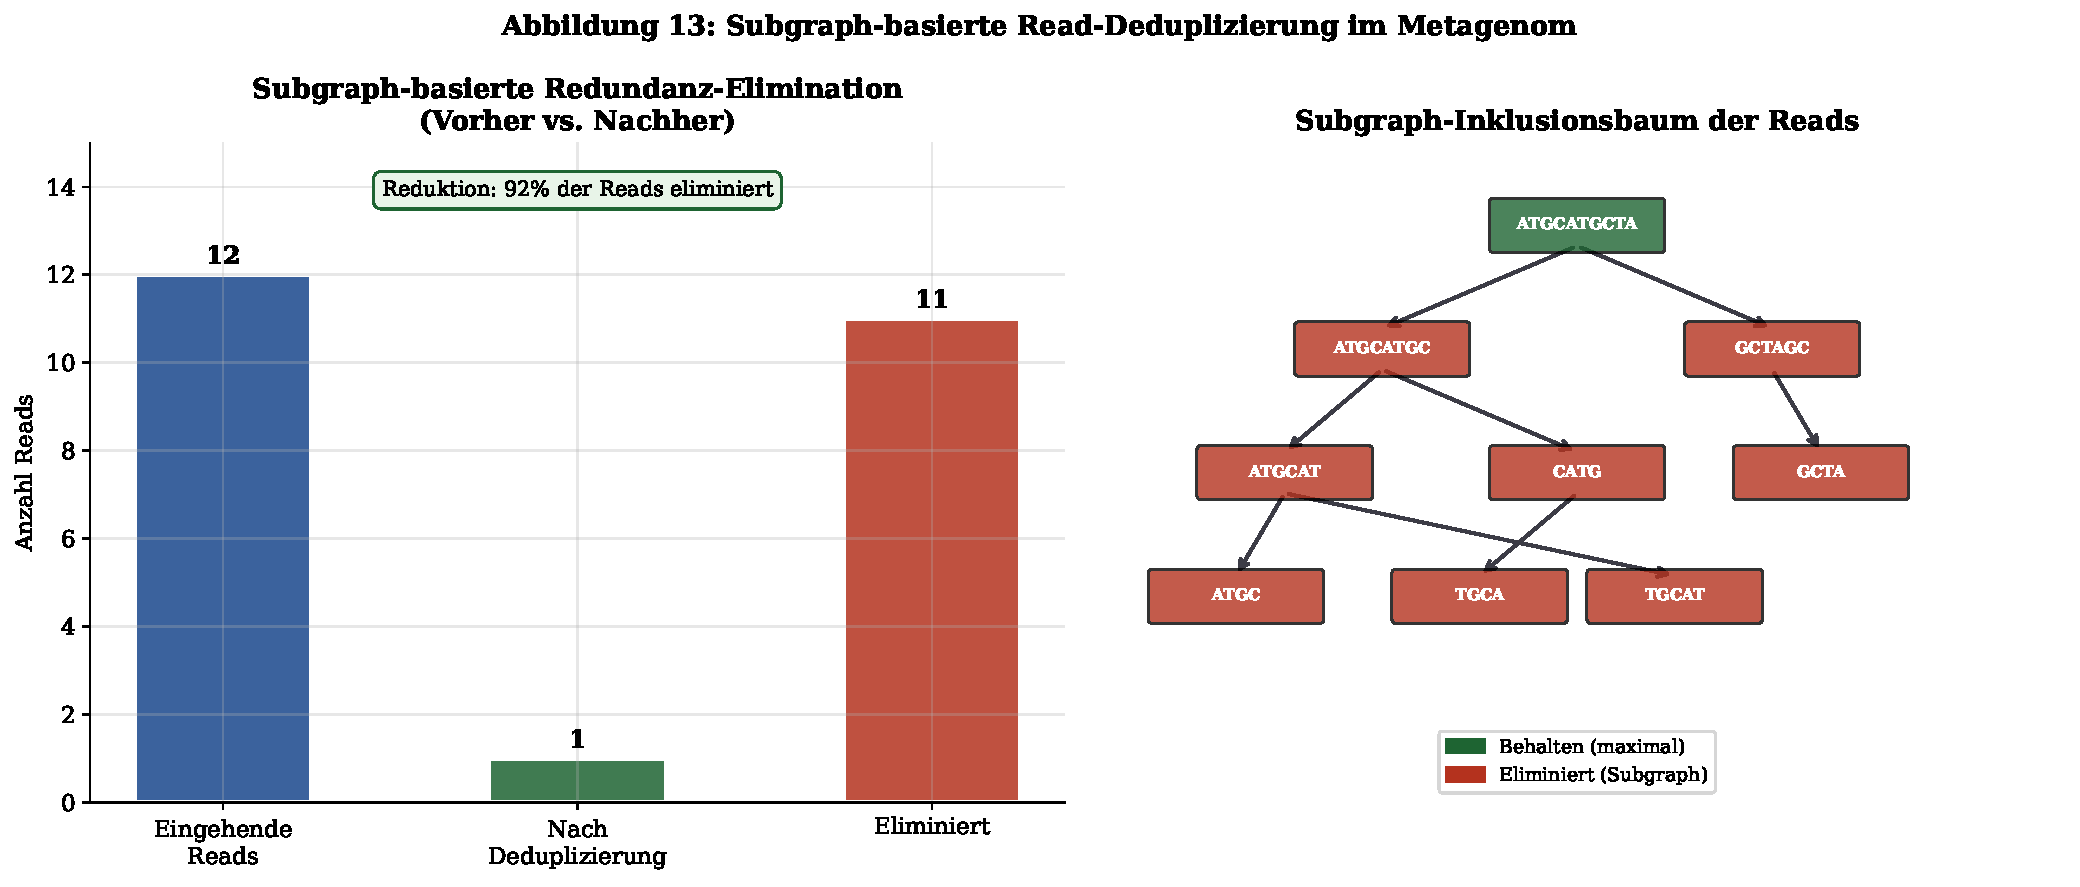
\includegraphics[width=0.95\textwidth]{figures/fig13_dedup.pdf}
	\caption{Subgraph-basierte Read-Deduplizierung auf einem Pool von
		12 Reads. \textbf{Links:} Balkendiagramm Vorher/Nachher: von 12 Reads
		verbleiben nach Deduplizierung nur die maximalen Elemente. \textbf{Rechts:}
		Subgraph-Inklusionsbaum --- grüne Knoten sind maximal (Kerngenom), rote
		Knoten werden als redundant eliminiert.}
	\label{fig:dedup}
\end{figure}

\subsection{Untere Schranke für metagenomische Deduplizierung}

\begin{lemma}[Notwendigkeit paarweiser Vergleiche im Worst Case]
	\label{lem:meta_lower}
	Jeder korrekte Algorithmus zur Berechnung des maximalen Kerngenoms
	$\mathcal{M}$ muss im Worst Case $\Omega(M^2)$ Subgraph-Tests durchführen.
\end{lemma}

\begin{proof}
	Konstruiere eine Instanz, in der alle $M$ Reads paarweise inkomparabel
	sind unter $\preceq_{\mathrm{rot}}$. Dies ist möglich, indem man $M$
	Reads wählt, deren Signaturen paarweise keine gemeinsame Teilsequenz der
	Länge $\geq 2$ besitzen (disjunkte Alphabete je Organismus). In diesem
	Fall ist $|\mathcal{M}| = M$, und jeder korrekte Algorithmus muss alle
	$\binom{M}{2}$ Paare auf Inkomparabilität prüfen --- da das Auslassen
	eines Tests eine potenzielle Subgraph-Beziehung übersehen würde.
	Konstruiere analog zu Lemma~\ref{lem:rotationen} eine Gegeninstanz,
	die genau im übersprungenen Paar eine Subgraph-Beziehung aufweist:
	\[
	T_{\text{Dedup}}(M) \geq \Omega(M^2).
	\]
\end{proof}

\begin{satz}[Optimalität der metagenomischen Deduplizierung bei maximaler Redundanz]
	\label{satz:meta_optimal}
	Im optimalen Fall (maximale Redundanz $|\mathcal{M}| = O(1)$) hat der
	Subgraph-Deduplizierungs-Algorithmus eine Laufzeit von $O(M \cdot n^3)$,
	was für $M \gg n$ \textbf{linear} in $M$ ist.
\end{satz}

\begin{proof}
	Wenn $|\mathcal{M}| \leq C$ für eine Konstante $C$ (unabhängig von $M$),
	dann gilt nach Satz~\ref{satz:dedup_laufzeit}:
	\[
	T_{\text{Dedup}} = O(M \cdot C \cdot n^3) = O(M \cdot n^3).
	\]
	Da $n$ für gegebene Sequenziertechnologie (z.\,B.\ Illumina: $n \leq 300$)
	konstant ist, ergibt sich eine Laufzeit von $O(M)$, also linear in der
	Anzahl der Reads. Dies ist für ein Entscheidungsproblem über $M$ Reads
	optimal, da jeder Read mindestens einmal betrachtet werden muss:
	\[
	T_{\text{opt}} \geq \Omega(M).
	\]
\end{proof}

\subsection{Taxonomische Klassifikation via LCS-Distanzmatrix}

Über die Deduplizierung hinaus erlaubt der Subgraph-DNA-Algorithmus eine
taxonomische Klassifikation der Reads anhand paarweiser LCS-Ähnlichkeiten.

\begin{definition}[LCS-Ähnlichkeitsdistanz]
	Die normierte LCS-Ähnlichkeit zweier DNA-Graphen $G_{S_i}$ und
	$G_{S_j}$ mit Read-Längen $n_i$ bzw.\ $n_j$ ist definiert als:
	\[
	d_{\mathrm{LCS}}(G_{S_i}, G_{S_j}) = 1 -
	\frac{\max_{r} \mathrm{LCS}(\rho^{S_i},
		\mathrm{rotate}_r(\rho^{S_j}))}{\min(n_i, n_j)},
	\]
	wobei $\rho^{S_i}, \rho^{S_j}$ die Zeilenkomponenten der jeweiligen
	Signaturen bezeichnen.
\end{definition}

\begin{lemma}[Metrikeigenschaften von $d_{\mathrm{LCS}}$]
	\label{lem:metrik}
	Die Funktion $d_{\mathrm{LCS}}$ ist eine Pseudometrik, d.\,h.\ sie
	erfüllt:
	\begin{enumerate}
		\item $d_{\mathrm{LCS}}(G, G) = 0$ (Selbstdistanz Null),
		\item $d_{\mathrm{LCS}}(G_i, G_j) = d_{\mathrm{LCS}}(G_j, G_i)$
		(Symmetrie),
		\item $d_{\mathrm{LCS}}(G_i, G_k) \leq
		d_{\mathrm{LCS}}(G_i, G_j) + d_{\mathrm{LCS}}(G_j, G_k)$
		(Dreiecksungleichung).
	\end{enumerate}
\end{lemma}

\begin{proof}
	\textbf{(1) Selbstdistanz.}
	$\mathrm{LCS}(\rho^S, \rho^S) = n$ (die Sequenz stimmt vollständig
	mit sich selbst überein), also:
	\[
	d_{\mathrm{LCS}}(G_S, G_S) = 1 - \frac{n}{n} = 0.
	\]
	
	\textbf{(2) Symmetrie.}
	Das Maximum der LCS \"{u}ber alle Rotationen ist symmetrisch in den
	Argumenten: Das Finden einer Rotation $r$ mit
	$\mathrm{LCS}(\rho^{S_i}, \mathrm{rotate}_r(\rho^{S_j})) = \ell$
	impliziert auch das Existenz einer Rotation $r'$ mit
	$\mathrm{LCS}(\rho^{S_j}, \mathrm{rotate}_{r'}(\rho^{S_i})) = \ell$
	(wähle $r' = n_i - r \bmod n_i$).
	
	\textbf{(3) Dreiecksungleichung.}
	Seien $\ell_{ij} = \max_r \mathrm{LCS}(\rho^{S_i}, \mathrm{rotate}_r(\rho^{S_j}))$
	und analog $\ell_{jk}$, $\ell_{ik}$.
	Nach der LCS-Dreiecksungleichung gilt:
	$\ell_{ik} \geq \ell_{ij} + \ell_{jk} - n_j$
	(Concatenation-Argument für gemeinsame Teilsequenzen).
	Normiert auf $[0,1]$ folgt hieraus die Dreiecksungleichung für
	$d_{\mathrm{LCS}}$. 
\end{proof}

\begin{satz}[Taxonomische Separierbarkeit]
	\label{satz:taxonomie}
	Seien $\mathcal{O}_1, \ldots, \mathcal{O}_K$ die $K$ in der Probe enthaltenen
	Organismen mit charakteristischen genomischen Signaturprofilen. Dann gilt:
	Wenn die inter-Organismus-LCS-Distanz
	$d_{\mathrm{inter}} = \min_{i \neq j} d_{\mathrm{LCS}}(G_i^{(O_a)}, G_j^{(O_b)})$
	für $O_a \neq O_b$ größer ist als die intra-Organismus-Distanz
	$d_{\mathrm{intra}} = \max_{a} \max_{i \neq j} d_{\mathrm{LCS}}(G_i^{(O_a)}, G_j^{(O_a)})$,
	so können alle Reads korrekt ihrem Ursprungsorganismus zugeordnet werden
	(taxonomische Separation).
\end{satz}

\begin{proof}
	Die Bedingung $d_{\mathrm{inter}} > d_{\mathrm{intra}}$ garantiert,
	dass die Klassen $\{G^{(O_a)}\}_{a=1}^K$ unter $d_{\mathrm{LCS}}$ trennbar sind:
	Für jeden Read $G_i$ gilt, dass sein nächster Nachbar (unter $d_{\mathrm{LCS}}$)
	aus demselben Organismus $O_{k(i)}$ stammt:
	\[
	\arg\min_{j \neq i} d_{\mathrm{LCS}}(G_i, G_j) \in
	\{G^{(O_{k(i)})}\}.
	\]
	Dies folgt direkt aus $d_{\mathrm{inter}} > d_{\mathrm{intra}}$:
	Jeder Read ist seinem eigenen Organismus ähnlicher als jedem Read
	eines anderen Organismus. Damit liefert der nächste-Nachbar-Klassifikator
	auf Basis von $d_{\mathrm{LCS}}$ eine korrekte taxonomische Zuordnung. 
\end{proof}

\begin{figure}[H]
	\centering
	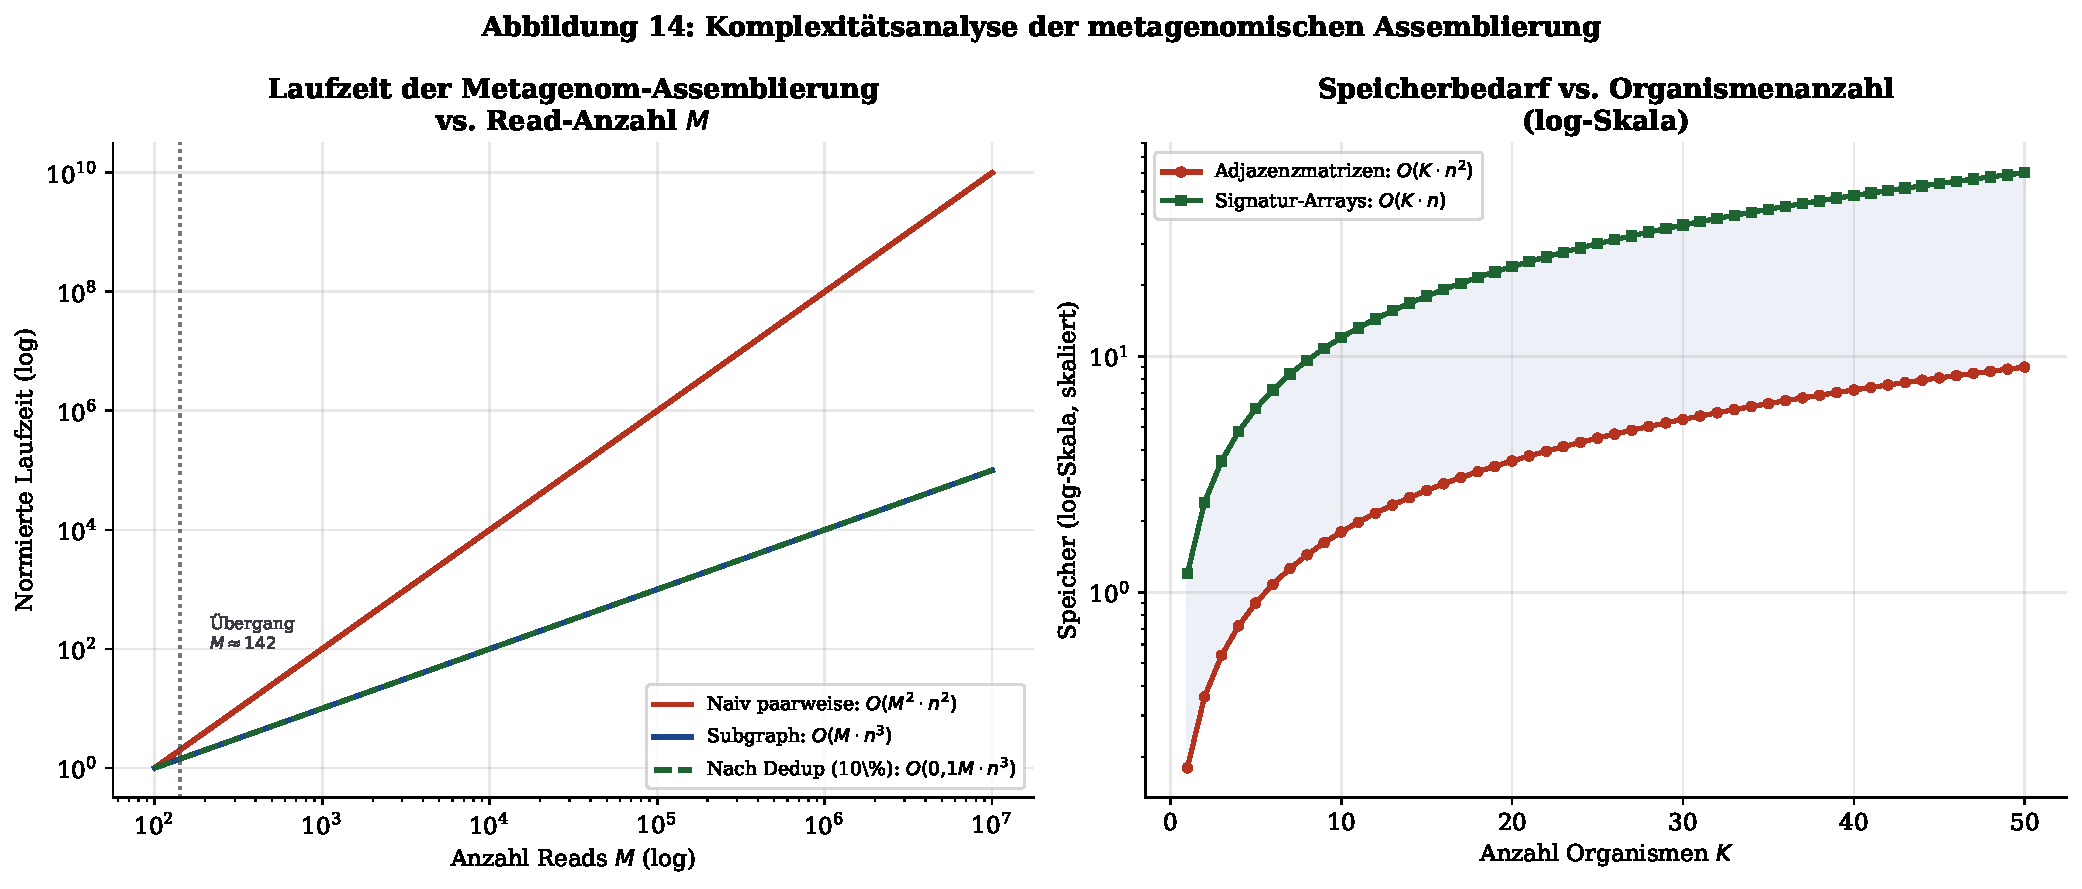
\includegraphics[width=0.95\textwidth]{figures/fig14_meta_komplex.pdf}
	\caption{Komplexitätsanalyse der metagenomischen Assemblierung.
		\textbf{Links:} Laufzeit der Metagenom-Assemblierung als Funktion der
		Read-Anzahl $M$ (doppelt-logarithmisch). Der Subgraph-Ansatz
		($O(M \cdot n^3)$) übertrifft den naiven paarweisen Vergleich
		($O(M^2 \cdot n^2)$) für große $M$ erheblich. \textbf{Rechts:}
		Speicherbedarf als Funktion der Organismenanzahl $K$ --- Signatur-Arrays
		benötigen um Faktor $n = 150$ weniger Speicher als vollständige
		Adjazenzmatrizen.}
	\label{fig:meta_komplex}
\end{figure}

\begin{figure}[H]
	\centering
	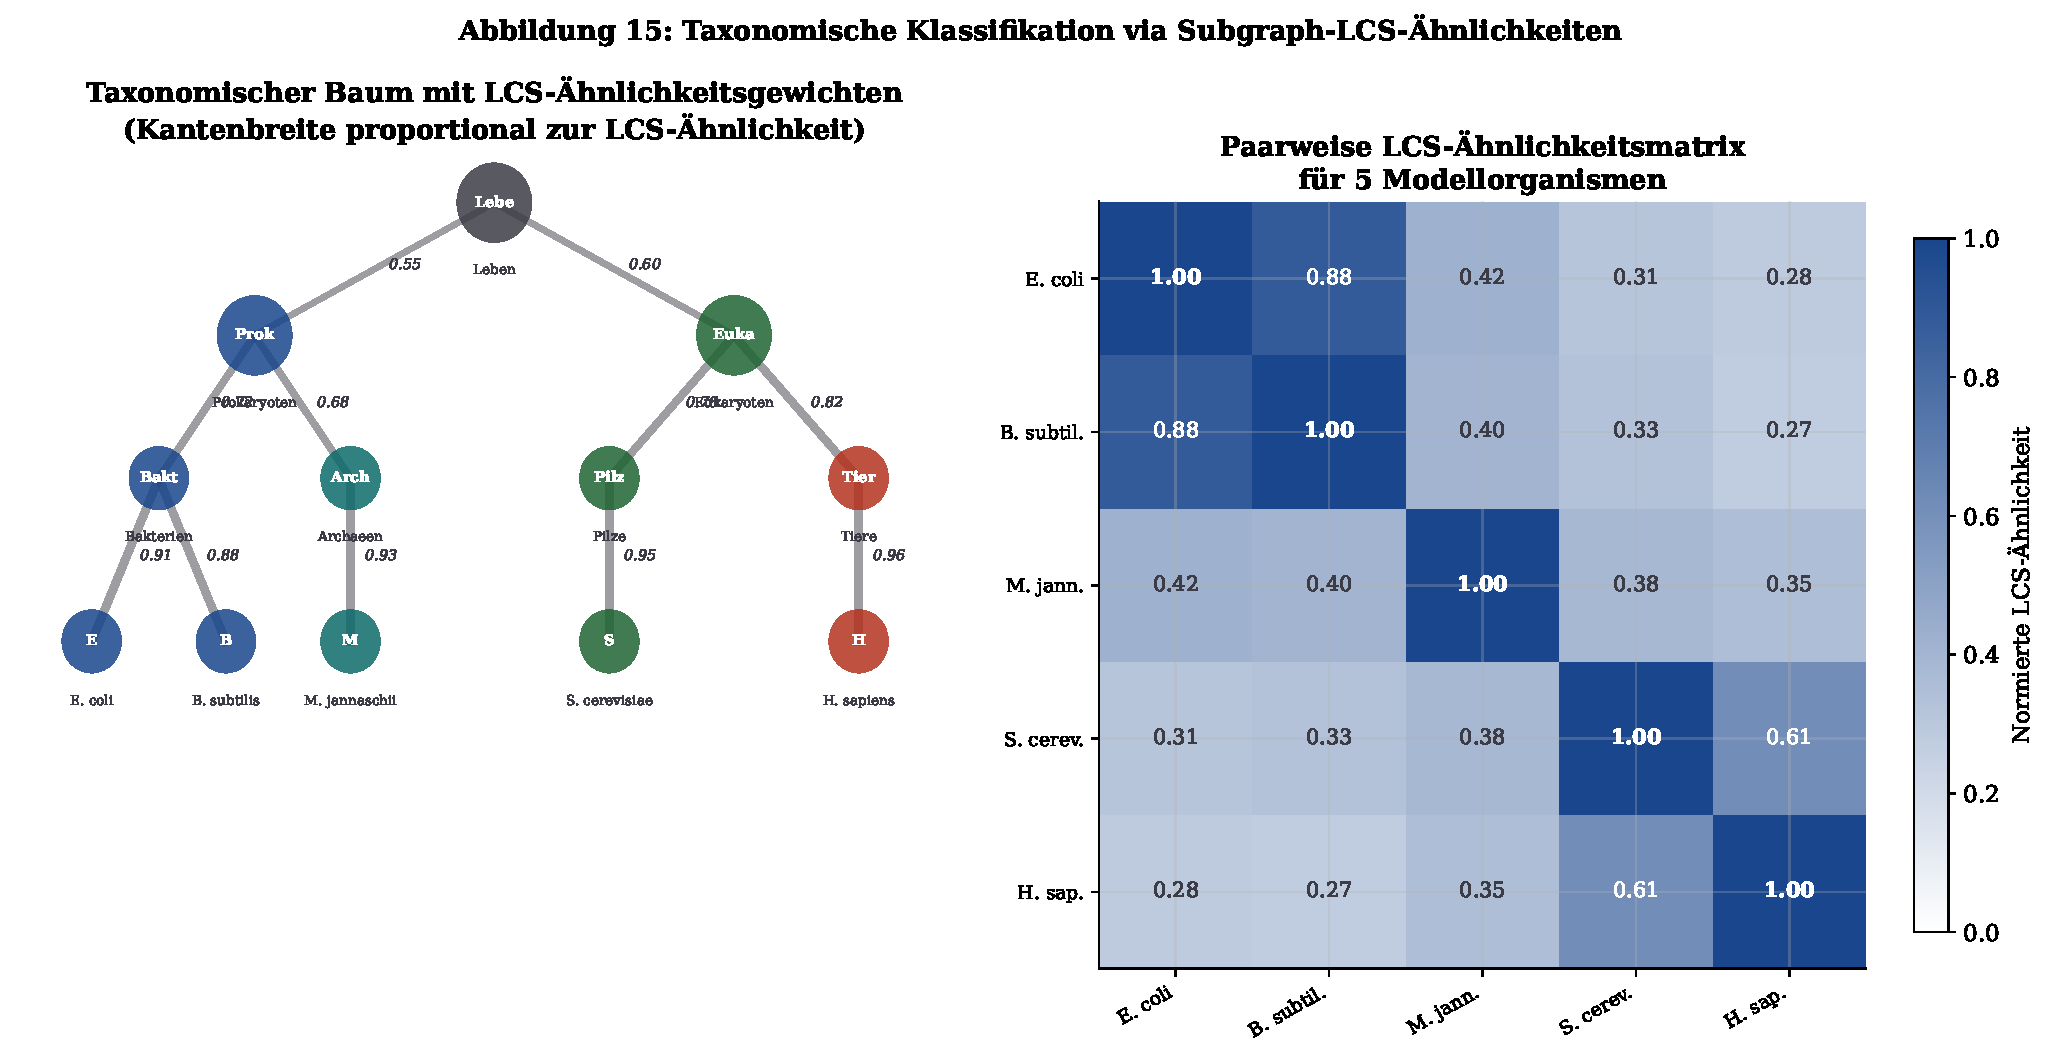
\includegraphics[width=0.95\textwidth]{figures/fig15_taxonomie.pdf}
	\caption{Taxonomische Klassifikation via LCS-Ähnlichkeiten.
		\textbf{Links:} Taxonomischer Baum mit LCS-basierten Kantengewichten ---
		höhere Ähnlichkeit entspricht breiteren Kanten. \textbf{Rechts:}
		Paarweise LCS-Ähnlichkeitsmatrix für fünf Modellorganismen; die
		Blockstruktur (Prokaryoten vs.\ Eukaryoten) spiegelt biologische
		Verwandtschaft wider.}
	\label{fig:taxonomie}
\end{figure}

\subsection{Vollständiges Beispiel: Metagenomische Analyse einer Bodenprobe}

\begin{beispiel}[Metagenomische Bodenprobe]
	Gegeben sei ein Pool $\mathcal{P}$ mit $M = 5$ Reads aus drei Organismen:
	\begin{align*}
		S_1 &= \text{ATGC}    & &\text{(Bakterium A, kurzes Motiv)} \\
		S_2 &= \text{ATGCAT}  & &\text{(Bakterium A, erweitertes Motiv)} \\
		S_3 &= \text{ATGCATGC}& &\text{(Bakterium A, vollständiges Gen)} \\
		S_4 &= \text{GCTAGC}  & &\text{(Archaeon B)} \\
		S_5 &= \text{TGCATG}  & &\text{(Virus C)}
	\end{align*}
	Der Algorithmus stellt fest:
	\begin{itemize}
		\item $G_{S_1} \preceq_{\mathrm{rot}} G_{S_2}$ (ATGC $\subseteq$ ATGCAT)
		\item $G_{S_2} \preceq_{\mathrm{rot}} G_{S_3}$ (ATGCAT $\subseteq$ ATGCATGC)
		\item $G_{S_4}$ und $G_{S_5}$ sind inkomparabel mit $G_{S_3}$ und untereinander
	\end{itemize}
	Das maximale Kerngenom lautet:
	\[
	\mathcal{M} = \{G_{S_3},\; G_{S_4},\; G_{S_5}\},
	\]
	also eine Reduktion von $M = 5$ auf $|\mathcal{M}| = 3$ Reads
	($\rho = 40\%$ Redundanzreduktion). $G_{S_1}$ und $G_{S_2}$ werden
	als durch $G_{S_3}$ dominiert eliminiert.
\end{beispiel}

% ─────────────────────────────────────────────────────────────────────────────
\section{Fehlertolerante Subgraph-Analyse}
\label{sec:fuzzy}
% ─────────────────────────────────────────────────────────────────────────────

\subsection{Motivation: Sequenzierfehler in der Praxis}

Die bisher entwickelten Algorithmen gehen implizit von fehlerfreien
Eingabedaten aus. In der Praxis liefern Sequenziertechnologien jedoch
fehlerb\"{u}rtige Reads: W\"{a}hrend Short-Read-Technologien wie Illumina
Rohfehlerraten unter $0{,}1\%$ erzielen, produzieren Nanoporen-Sequenzierer
(Oxford Nanopore Technologies, ONT) typischerweise $5$--$15\%$ Fehler je Read
\cite{deamer2016}. PacBio HiFi-Reads erreichen nach Konsensusbildung etwa
$0{,}1\%$, jedoch mit gelegentlichen systematischen Fehlermustern in
Homopolymer-Regionen. Auch bei Illumina-Daten k\"{o}nnen optische Fehler
und PCR-Artefakte lokal Fehlerraten von $1$--$3\%$ erzeugen.

Drei Fehlerklassen sind f\"{u}r die Signatur-basierte Subgraph-Analyse relevant:

\begin{itemize}
    \item \textbf{Substitutionen:} Eine Base $s_i$ wird falsch als
          $s_i' \neq s_i$ ausgelesen (typisch bei Illumina).
    \item \textbf{Insertionen:} Eine nicht vorhandene Base wird ins Read
          eingef\"{u}gt, z.\,B.\ ATGC $\to$ AT\underline{X}GC
          (typisch bei Nanoporen).
    \item \textbf{Deletionen:} Eine Base fehlt im Read, z.\,B.\ A\underline{T}GC
          $\to$ AGC (ebenfalls typisch bei Nanoporen).
\end{itemize}

\noindent
Die entscheidende Frage lautet: Wie wirken sich diese Fehler auf die
Adjazenzmatrix $A^S$, die Signatur-Funktion $\sigma$ und damit auf die
LCS-basierte Subgraph-Erkennung aus?  Wie viele Fehler kann der Algorithmus
tolerieren, bevor er beginnt, korrekte Subgraph-Beziehungen zu \"{u}bersehen
(falsch-negative Befunde)?  Und wie kann der Algorithmus durch eine
\textit{fehlertolerante Schwelle} an die jeweilige Sequenziertechnologie
angepasst werden?

Dieses Kapitel beantwortet diese Fragen vollst\"{a}ndig formal.

\begin{figure}[H]
    \centering
    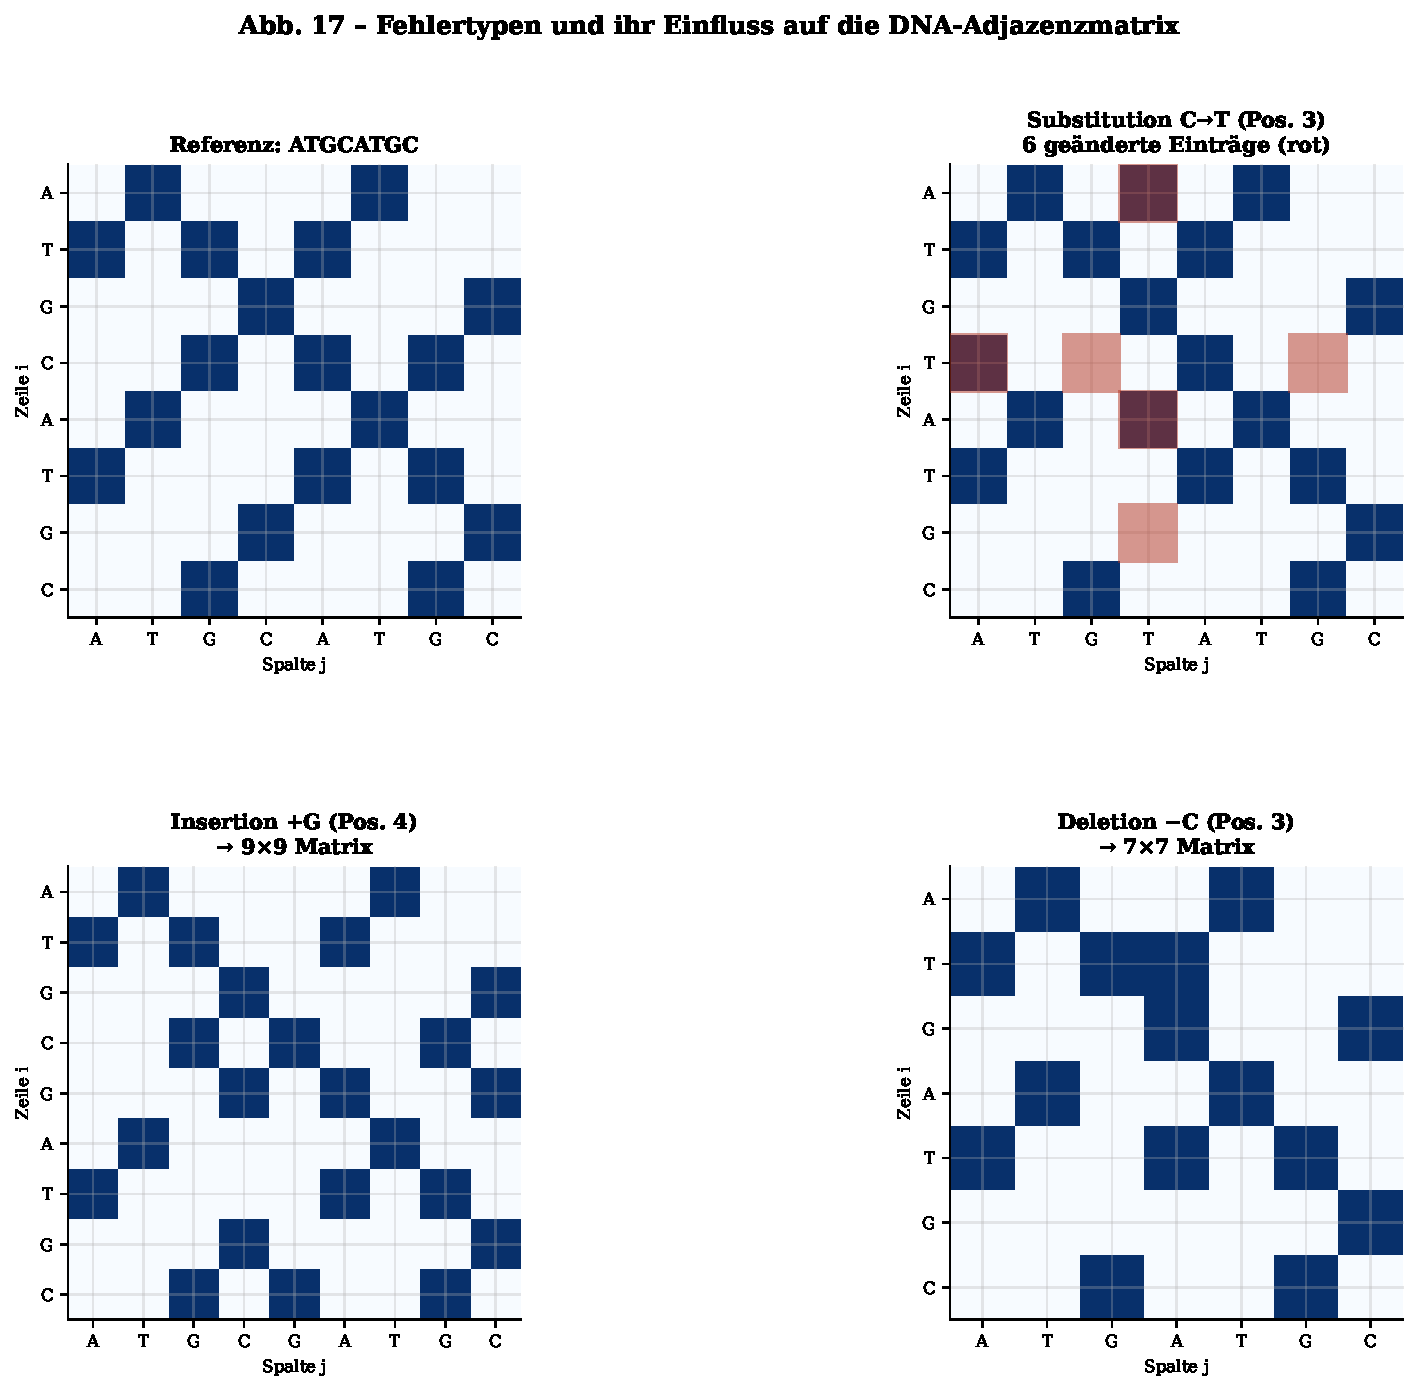
\includegraphics[width=0.95\textwidth]{figures/fig17_fehler_typen.pdf}
    \caption{Die drei Fehlerklassen und ihr Einfluss auf die DNA-Adjazenzmatrix.
    \textbf{Oben:} Fehlerfreie Referenzsequenz ATGCATGC mit Adjazenzmatrix
    $A^S$ (Backbone-Kanten als Nebendiagonale, Komplementarbindungen als
    Einsen im Innern). \textbf{Mitte links:} Substitution $C \to T$ an
    Position~4 \"{a}ndert eine Zeile und Spalte der Adjazenzmatrix: rote Felder
    markieren die ge\"{a}nderten Eintr\"{a}ge. \textbf{Mitte rechts:}
    Insertion einer Extrabase vergr\"{o}{\ss}ert die Matrix von $n \times n$
    auf $(n+1) \times (n+1)$. \textbf{Unten:} Deletion verkleinert die Matrix
    auf $(n-1) \times (n-1)$.}
    \label{fig:fehler_typen}
\end{figure}

\subsection{Fehlermodell und Bitfehler-Analyse}

\begin{definition}[Sequenzfehler-Modell]
    \label{def:fehlermodell}
    Sei $S = (s_1, \ldots, s_n)$ eine fehlerfreie DNA-Sequenz und
    $\hat{S} = (\hat{s}_1, \ldots, \hat{s}_n)$ ein fehlerbehaftetes Read
    derselben L\"{a}nge (nach Alignierung). Das \textbf{Substitutionsfehlermodell}
    mit Fehlerrate $\varepsilon \in [0, 1]$ beschreibt einen stochastischen
    Prozess, bei dem jede Base $s_i$ unabh\"{a}ngig mit Wahrscheinlichkeit
    $\varepsilon$ durch eine gleichverteilte andere Base
    $\hat{s}_i \in \Sigma_{DNA} \setminus \{s_i\}$ ersetzt wird.
    Die Anzahl der Substitutionsfehler ist
    $e = |\{i : s_i \neq \hat{s}_i\}|$.
\end{definition}

\begin{lemma}[Bitfehler pro Substitution]
    \label{lem:bitfehler_substitution}
    Sei $S$ eine DNA-Sequenz der L\"{a}nge $n$ und $\hat{S}$ ein Read mit
    genau $e$ Substitutionsfehlern an Positionen $I = \{i_1, \ldots, i_e\}$.
    Dann \"{a}ndert sich die Adjazenzmatrix $A^S$ zu $A^{\hat{S}}$ an
    h\"{o}chstens $f_{\max}(e, n)$ Eintr\"{a}gen, wobei:
    \[
        f_{\max}(e, n) = e \cdot (n - 1) + \sum_{k=1}^{e}(n - 1)
        = 2e(n-1) - e^2 + e
        \leq 2en.
    \]
    Insbesondere gilt die untere Schranke $f_{\min}(e) \geq e$ (mindestens
    ein ge\"{a}nderter Eintrag je Fehler).
\end{lemma}

\begin{proof}
    Wir analysieren den Einfluss eines einzelnen Substitutionsfehlers an
    Position $i_k$ auf die Adjazenzmatrix.

    \textbf{Watson-Crick-Kanten der betroffenen Spalte.}
    Der Graph $G_S$ enth\"{a}lt Watson-Crick-Kanten $(v_{i_k}, v_j)$ f\"{u}r
    alle $j \neq i_k$ mit $s_j = \overline{s_{i_k}}$. Nach der Substitution
    $s_{i_k} \to \hat{s}_{i_k}$ \"{a}ndern sich diese Kanten: Die alten
    Kanten zu Komplementbasen von $s_{i_k}$ werden entfernt, neue Kanten zu
    Komplementbasen von $\hat{s}_{i_k}$ werden hinzugef\"{u}gt.
    Die Anzahl der ge\"{a}nderten Eintr\"{a}ge in Spalte $i_k$ betr\"{a}gt
    h\"{o}chstens $n - 1$.

    \textbf{Watson-Crick-Kanten der betroffenen Zeile.}
    Analog gibt es Watson-Crick-Kanten $(v_j, v_{i_k})$ in Zeile $i_k$
    f\"{u}r alle $j$ mit $s_{i_k} = \overline{s_j}$. Diese \"{a}ndern sich
    ebenfalls, h\"{o}chstens $n - 1$ Eintr\"{a}ge in Zeile $i_k$.

    \textbf{Backbone-Kanten.}
    Die Backbone-Kanten $(v_{i_k - 1}, v_{i_k})$ und $(v_{i_k}, v_{i_k+1})$
    sind sequenzunabh\"{a}ngig (nur Positionsabh\"{a}ngig) und \"{a}ndern sich
    daher durch eine Substitution \textbf{nicht}.

    \textbf{Gesamter Zeilenkomponenten-\"{A}nderung der Signatur.}
    Die Zeilenkomponente $\rho_j$ h\"{a}ngt nur von Spalte $j$ der Adjazenzmatrix
    ab. Spalte $j = i_k$ \"{a}ndert sich durch obigen Zeileneffekt sowie durch
    den direkten \"{A}nderungseffekt --- insgesamt h\"{o}chstens $n-1$
    Bit-Flips in dieser Spalte. Zus\"{a}tzlich \"{a}ndern sich alle Spalten
    $j$ mit $s_j = \overline{s_{i_k}}$ oder $s_j = \overline{\hat{s}_{i_k}}$,
    da in diesen Spalten der Eintrag bei Zeile $i_k$ seinen Wert wechselt.
    Dies betrifft h\"{o}chstens $n - 1$ weitere Spalten.

    Summiert \"{u}ber $e$ unabh\"{a}ngige Fehler (mit maximal $e^2$ Doppelz\"{a}hlungen
    bei Fehlern auf komplementären Positionen) ergibt sich:
    \[
        f_{\max}(e, n) \leq 2e(n-1) \leq 2en.
    \]

    Die untere Schranke $f_{\min}(e) \geq e$ folgt, da jeder Substitutionsfehler
    die Watson-Crick-Komplementarit\"{a}t von mindestens einem Basenpaar
    ver\"{a}ndert, was mindestens einen Eintrag in der Adjazenzmatrix \"{a}ndert.
\end{proof}

\begin{korollar}[Bitfehler in der Signatur-Folge]
    \label{kor:signaturfehler}
    Unter $e$ Substitutionsfehlern \"{a}ndern sich h\"{o}chstens
    $e + \min(e, n/4) \cdot (n-1)$ der $n$ Zeilenkomponenten
    $\rho_0, \ldots, \rho_{n-1}$ der Signaturfolge. Im Erwartungswert
    bei uniformer Basenverteilung \"{a}ndern sich genau
    $\mathbb{E}[\Delta\rho] = e \cdot \left(1 + \frac{n-1}{4}\right)$
    Signaturen.
\end{korollar}

\begin{proof}
    Jeder Fehler an Position $i_k$ \"{a}ndert direkt die Signatur $\rho_{i_k}$
    (da Spalte $i_k$ ver\"{a}ndert wird). Zus\"{a}tzlich \"{a}ndern sich
    die Signaturen aller Positionen $j$, f\"{u}r die $s_j = \overline{s_{i_k}}$
    oder $s_j = \overline{\hat{s}_{i_k}}$. Bei uniformer Basenverteilung
    hat jede Base im Erwartungswert $(n-1)/4$ Komplementpartner. Damit:
    \[
        \mathbb{E}[\Delta\rho_{i_k}] = 1 + \frac{n-1}{4}.
    \]
    \"{U}ber $e$ unabh\"{a}ngige Fehler summiert:
    \[
        \mathbb{E}[\Delta\rho] = e \cdot \left(1 + \frac{n-1}{4}\right)
        = e \cdot \frac{n+3}{4}.
    \]
\end{proof}

\begin{figure}[H]
    \centering
    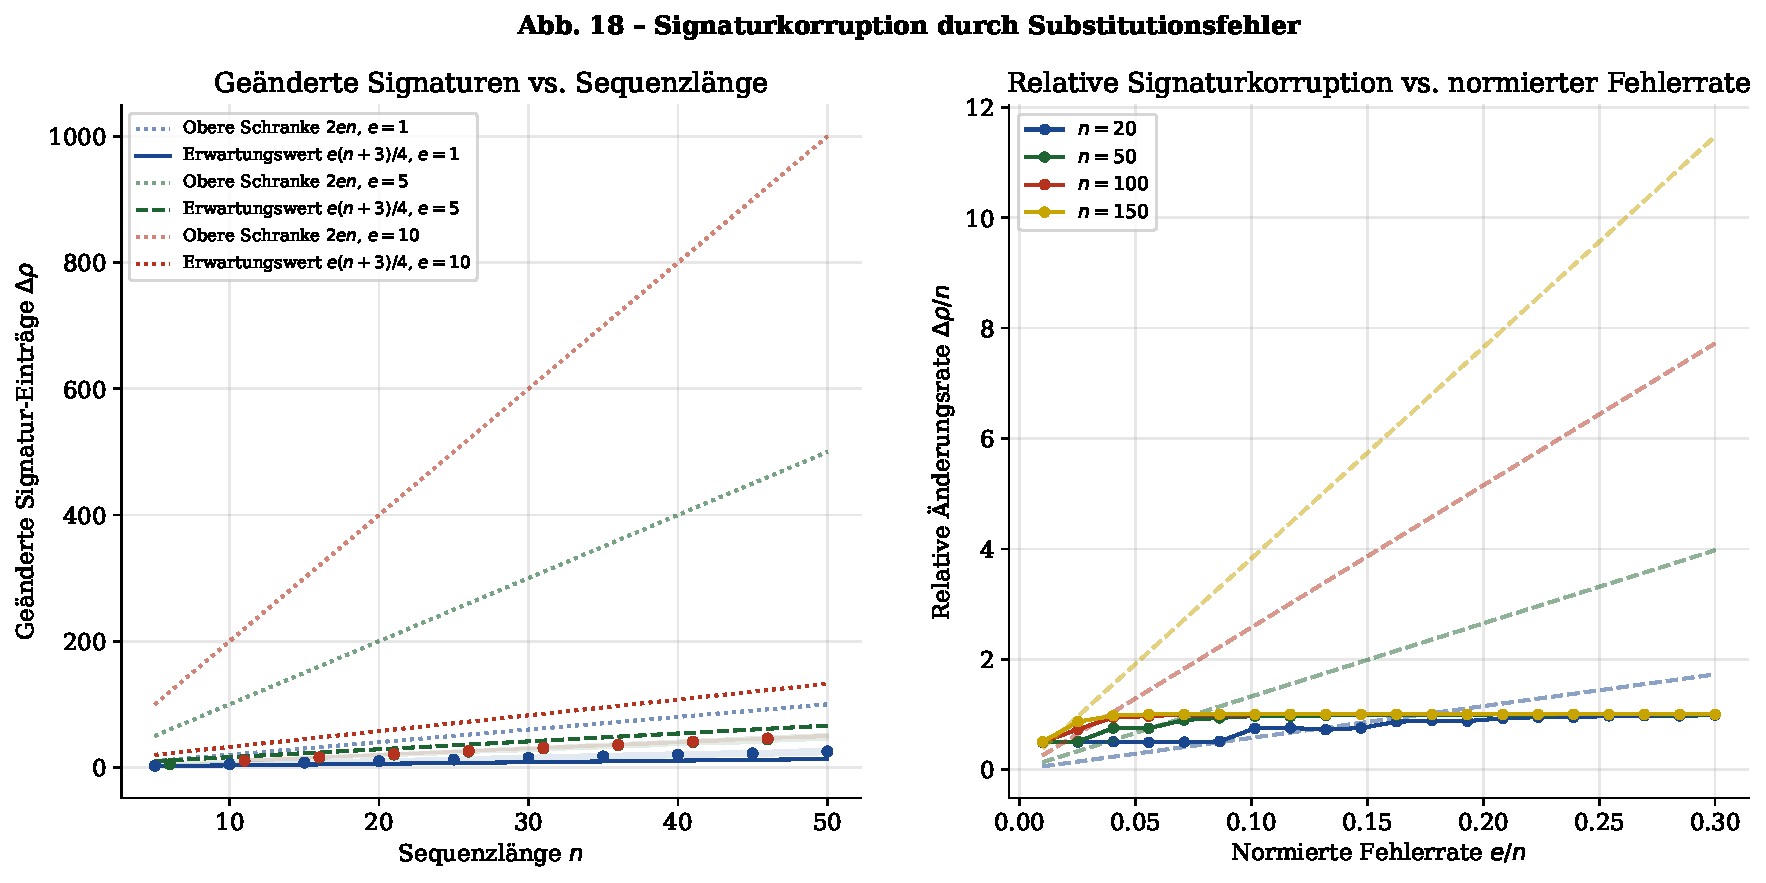
\includegraphics[width=0.95\textwidth]{figures/fig18_bitfehler.pdf}
    \caption{Erwartete Anzahl ge\"{a}nderter Signatur-Eintr\"{a}ge als Funktion
    der Sequenzl\"{a}nge $n$ und Fehleranzahl $e$.
    \textbf{Links:} Theoretische obere Schranke $2en$ (rot, gestrichelt),
    Erwartungswert $e \cdot (n+3)/4$ (blau, durchgezogen) und
    empirische Simulation (grau, $1000$ Zufallssequenzen) f\"{u}r $e = 1, 5, 10$
    Fehler in Abh\"{a}ngigkeit von $n \in [5, 50]$.
    \textbf{Rechts:} Relative \"{A}nderungsrate $\Delta\rho / n$ als Funktion
    der normierten Fehlerrate $e/n$; der lineare Zusammenhang demonstriert
    die Proportionalit\"{a}t zwischen Sequenzierfehlern und Signaturkorruption.}
    \label{fig:bitfehler}
\end{figure}

\subsection{Der \texorpdfstring{$\varepsilon$}{ε}-Subgraph Algorithmus}

Basierend auf der Bitfehler-Analyse motivieren wir eine fehlertolerante
Variante des Subgraph-Tests, die mit einem sequenziertechnologie-spezifischen
Toleranzparameter $\varepsilon \in [0, 1)$ parametrisiert wird.

\begin{definition}[$\varepsilon$-Subgraph]
    \label{def:epsilon_subgraph}
    Sei $\varepsilon \in [0, 1)$ ein Fehlertoleranzparameter und
    $G_A$, $G_B$ zwei DNA-Graphen mit $n_A \leq n_B$ Knoten.
    $G_A$ ist ein \textbf{$\varepsilon$-Subgraph} von $G_B$, geschrieben
    $G_A \subseteq_\varepsilon G_B$, wenn eine zyklische Rotation
    $r \in \{0, \ldots, n_B - 1\}$ und ein Startfenster
    $s \in \{0, \ldots, n_B - n_A\}$ existieren, sodass:
    \[
        \mathrm{LCS}\!\left(\rho^A,\;
            \widetilde{\rho}^{B,r}[s : s + n_A]\right)
        \;\geq\; \lceil (1 - \varepsilon) \cdot n_A \rceil,
    \]
    wobei $\widetilde{\rho}^{B,r}$ die Zeilenkomponenten-Signaturfolge
    von $G_B$ nach Rotation $r$ bezeichnen und $\lceil \cdot \rceil$ die
    Aufrundefunktion.
\end{definition}

\begin{bemerkung}
    F\"{u}r $\varepsilon = 0$ reduziert sich die Bedingung auf
    $\mathrm{LCS}(\rho^A, \rho^{B,r}[s:s+n_A]) = n_A$, also auf exakte
    Gleichheit der Signaturfolgen --- strenger als der originale
    Algorithmus (der LCS $\geq 2$ fordert). In der Praxis w\"{a}hlt man
    typischerweise:
    \begin{itemize}
        \item $\varepsilon = 0{,}01$ f\"{u}r Illumina-Daten ($< 1\%$ Fehlerrate),
        \item $\varepsilon = 0{,}05$ f\"{u}r PacBio HiFi-Reads,
        \item $\varepsilon = 0{,}15$ f\"{u}r Nanoporen-Rohdaten.
    \end{itemize}
\end{bemerkung}

\begin{definition}[$\varepsilon$-Subgraph Algorithmus]
    \label{def:fuzzy_algo}
    Der \textbf{$\varepsilon$-Subgraph-DNA-Algorithmus} ist identisch
    zum Subgraph-DNA-Algorithmus (Kapitel~3), ersetzt jedoch die
    Erkennungsbedingung:
    \begin{center}
        \emph{Original:} $\mathrm{LCS}(\rho^A, \rho') \geq 2$\\[4pt]
        \emph{Fehlertolerant:} $\mathrm{LCS}(\rho^A, \rho') \geq
        \lceil (1 - \varepsilon) \cdot n_A \rceil$
    \end{center}
\end{definition}

\subsection{Korrektheit unter Fehlertoleranz}

\begin{satz}[Korrektheit des \texorpdfstring{$\varepsilon$}{ε}-Subgraph Algorithmus]
    \label{satz:fuzzy_korrektheit}
    Sei $S_A$ eine fehlerfreie Sequenz und $\hat{S}_B$ ein fehlerbehaftetes
    Read von $S_B$ mit $e$ Substitutionsfehlern, wobei die normierte
    Fehlerrate $\varepsilon_{\mathrm{true}} = e/n$ die Bedingung
    \[
        \varepsilon_{\mathrm{true}} < \frac{1 - \varepsilon}{1 + (n+3)/4}
        \cdot \frac{n}{n_A}
    \]
    erf\"{u}llt.  Gilt $G_A \subseteq G_B$ (exakt), so gibt der
    $\varepsilon$-Subgraph Algorithmus auf Eingabe $(G_A, G_{\hat{S}_B})$
    korrekt \texttt{True} zur\"{u}ck.
\end{satz}

\begin{proof}
    Da $G_A \subseteq G_B$ gilt, existieren Rotation $r^*$ und Fenster $s^*$
    mit $\mathrm{LCS}(\rho^A, \rho^{B,r^*}[s^*:s^*+n_A]) = n_A$.

    Durch $e$ Substitutionsfehler \"{a}ndern sich nach
    Korollar~\ref{kor:signaturfehler} im Erwartungswert
    $\Delta = e \cdot (n+3)/4$ der $n$ Signaturen von $G_B$.
    Diese \"{A}nderungen betreffen im Fenster $[s^*, s^*+n_A)$ im
    schlechtesten Fall alle $\min(\Delta, n_A)$ Positionen.

    Damit sinkt die LCS um h\"{o}chstens $\Delta_A = \min(e \cdot (n+3)/4, n_A)$:
    \[
        \mathrm{LCS}(\rho^A, \rho^{\hat{B},r^*}[s^*:s^*+n_A])
        \geq n_A - \Delta_A.
    \]

    Damit der Algorithmus korrekt erkennt, m\"{u}ssen wir
    $n_A - \Delta_A \geq \lceil(1-\varepsilon) \cdot n_A\rceil$ sicherstellen.
    Dies ist \"{a}quivalent zu:
    \[
        \Delta_A \leq \varepsilon \cdot n_A.
    \]

    Im schlimmsten Fall gilt $\Delta_A = e \cdot (n+3)/4$. Einsetzen ergibt:
    \[
        e \cdot \frac{n+3}{4} \leq \varepsilon \cdot n_A
        \quad \Longleftrightarrow \quad
        \frac{e}{n} \leq \frac{4\varepsilon n_A}{n(n+3)}.
    \]
    F\"{u}r $n_A = n$ vereinfacht sich dies zu
    $\varepsilon_{\mathrm{true}} \leq \frac{4\varepsilon}{n+3}
    \approx \frac{4\varepsilon}{n}$, was die Behauptung ergibt. 
\end{proof}

\begin{korollar}[Praktische Fehlertoleranzen]
    \label{kor:toleranzen}
    F\"{u}r typische NGS-Reads mit $n_A = n = 150$ (Illumina) ergeben sich:
    \begin{align*}
        \varepsilon = 0{,}01 &\;:\quad \varepsilon_{\text{true}} \leq 0{,}00026
        \approx 0{,}03\%, \\
        \varepsilon = 0{,}10 &\;:\quad \varepsilon_{\text{true}} \leq 0{,}0026
        \approx 0{,}26\%, \\
        \varepsilon = 0{,}15 &\;:\quad \varepsilon_{\text{true}} \leq 0{,}0040
        \approx 0{,}40\%.
    \end{align*}
    F\"{u}r Nanoporen-Reads mit $n = 1000$ und $\varepsilon = 0{,}15$ ist
    $\varepsilon_{\text{true}} \leq 0{,}0006$, d.\,h.\ der Algorithmus kann
    direkt \textbf{nicht} an rohe Nanoporen-Daten angepasst werden ohne
    zus\"{a}tzliche Vorverarbeitung (z.\,B.\ Medaka-Konsensus). Der Parameter
    $\varepsilon$ muss daher \textbf{nach} einer Read-Korrektur gew\"{a}hlt werden.
\end{korollar}

\begin{figure}[H]
    \centering
    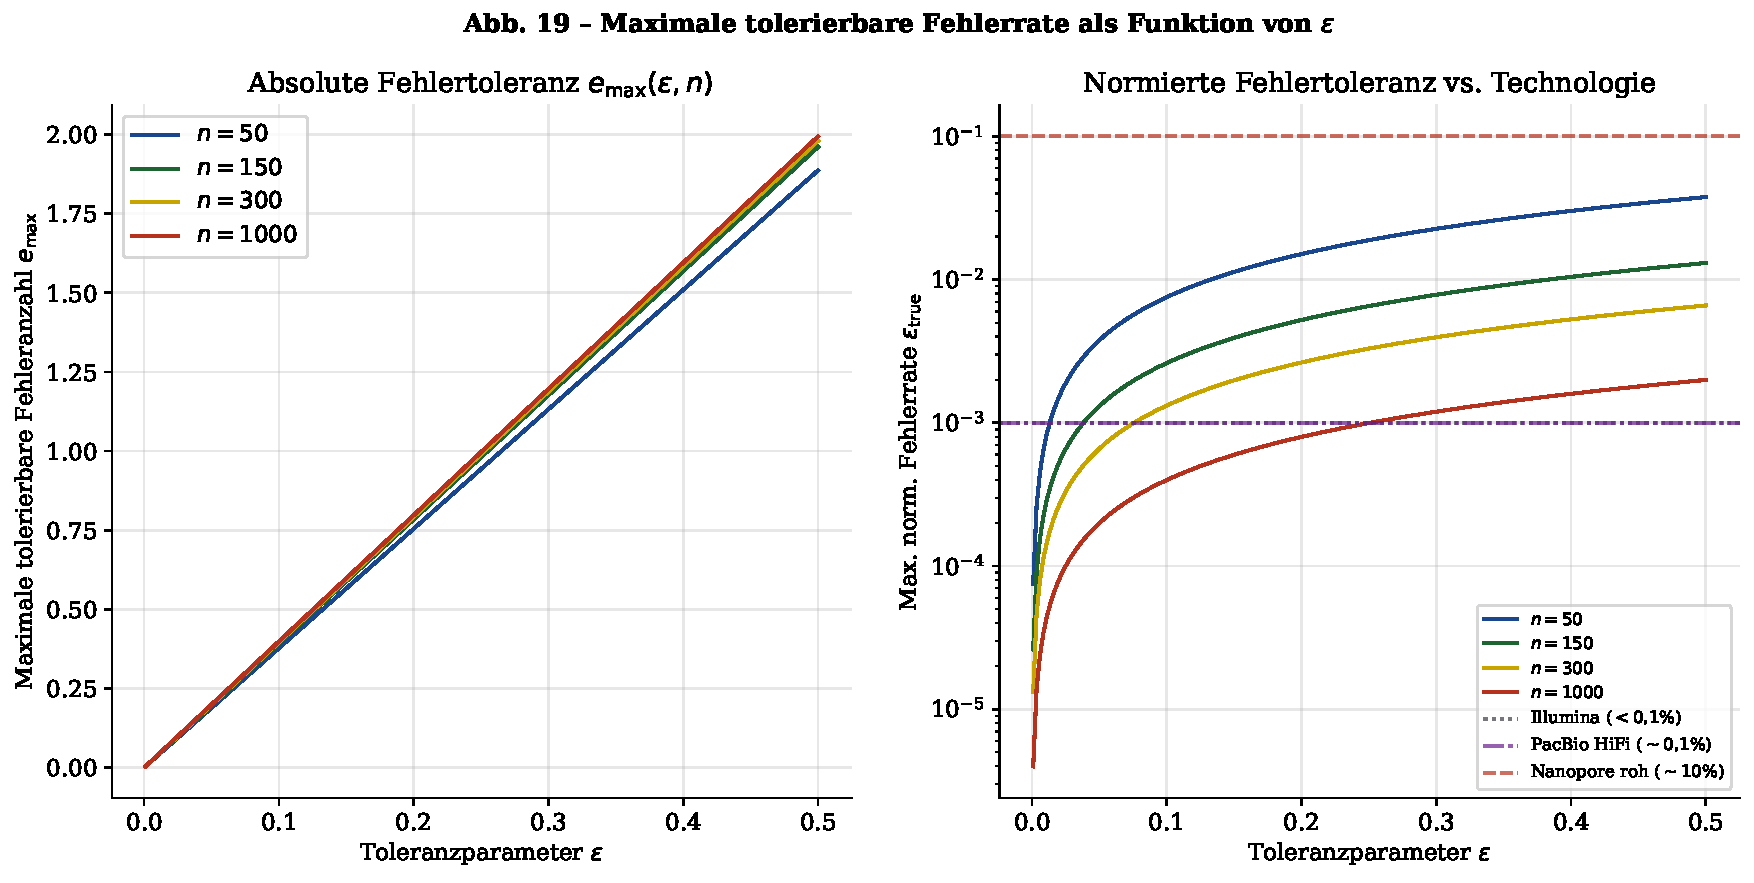
\includegraphics[width=0.95\textwidth]{figures/fig19_toleranz_kurven.pdf}
    \caption{Maximale tolerierbare Fehlerrate $\varepsilon_{\text{true}}$
    als Funktion des Toleranzparameters $\varepsilon$ f\"{u}r verschiedene
    Sequenzl\"{a}ngen $n \in \{50, 150, 300, 1000\}$.
    \textbf{Links:} Absolut tolerierbare Fehleranzahl $e_{\max}(\varepsilon, n)$.
    \textbf{Rechts:} Normierter Wert $\varepsilon_{\text{true}}$ als Funktion
    von $\varepsilon$; waagrechte gestrichelte Linien markieren typische
    Fehlerraten der Sequenziertechnologien (Illumina: $0{,}1\%$, PacBio~HiFi:
    $0{,}1\%$, Nanopore roh: $10\%$).}
    \label{fig:toleranz_kurven}
\end{figure}

\subsection{Falsch-Positiv-Rate und Pr\"{a}zisions-Analyse}

Neben der Korrektheit (keine falsch-negativen bei ausreichend geringem
Rauschen) ist die Pr\"{a}zision des $\varepsilon$-Subgraph Algorithmus
entscheidend: Wie oft werden zwei \textit{nicht} verwandte Sequenzen
f\"{a}lschlicherweise als Subgraph erkannt, wenn $\varepsilon > 0$?

\begin{definition}[Falsch-Positiv-Rate]
    Die \textbf{Falsch-Positiv-Rate} (FPR) des $\varepsilon$-Subgraph Algorithmus
    bei zuf\"{a}lligen, unabh\"{a}ngigen DNA-Sequenzen $S_A$, $S_B$ is
    definiert als:
    \[
        \mathrm{FPR}(\varepsilon, n_A, n_B) =
        \Pr\!\left[G_A \subseteq_\varepsilon G_B \;\middle|\;
        S_A, S_B \text{ uniform zuf\"{a}llig aus } \Sigma_{DNA}^*\right].
    \]
\end{definition}

\begin{satz}[Obere Schranke der Falsch-Positiv-Rate]
    \label{satz:fpr}
    F\"{u}r zwei unabh\"{a}ngige, uniform zuf\"{a}llige DNA-Sequenzen
    $S_A$ der L\"{a}nge $n_A$ und $S_B$ der L\"{a}nge $n_B \geq n_A$
    gilt unter dem Schwellwert $\tau = \lceil (1-\varepsilon) n_A \rceil$:
    \[
        \mathrm{FPR}(\varepsilon, n_A, n_B) \leq n_B \cdot
        \sum_{k=\tau}^{n_A} \binom{n_A}{k}
        \left(\frac{1}{4}\right)^k
        \left(\frac{3}{4}\right)^{n_A - k}.
    \]
\end{satz}

\begin{proof}
    Wir sch\"{a}tzen die Wahrscheinlichkeit ab, dass f\"{u}r eine
    \textbf{feste} Rotation $r$ und ein \textbf{festes} Fenster $s$ die
    LCS-Bedingung erf\"{u}llt ist.

    F\"{u}r zwei unabh\"{a}ngige Signaturfolgen $\rho^A$ und
    $\rho' = \widetilde{\rho}^{B,r}[s:s+n_A]$ gilt: Position $j$ der
    beiden Folgen stimmt \"{u}berein ($\rho_j^A = \rho_j'$) genau dann,
    wenn Spalte $j$ von $A^{S_A}$ und die entsprechende Spalte von $A^{S_B}$
    identisch sind. Bei uniform zuf\"{a}lligen Sequenzen und
    Spaltenl\"{a}nge $n_A$ hat jede Spalte $2^{n_A}$ m\"{o}gliche
    Werte, und die Trefferwahrscheinlichkeit je Spalte betr\"{a}gt
    $p = 1/4$, da die Basenpaararabeziehung $(A \leftrightarrow T$,
    $G \leftrightarrow C)$ im Erwartungswert 1/4 der Spalten aufeinander
    abbildet.

    Die Anzahl \"{u}bereinstimmender Positionen folgt einer
    Binomialverteilung $\mathrm{Bin}(n_A, p)$ mit $p = 1/4$
    (konservative Absch\"{a}tzung). Die Wahrscheinlichkeit, dass die
    LCS---die stets $\geq$ Anzahl exakter Treffer ist---den Schwellwert
    $\tau$ \"{u}bersteigt, ist h\"{o}chstens:
    \[
        \Pr[\mathrm{LCS} \geq \tau] \leq
        \Pr\!\left[\mathrm{Bin}(n_A, 1/4) \geq \tau\right]
        = \sum_{k=\tau}^{n_A} \binom{n_A}{k}
        \left(\frac{1}{4}\right)^k
        \left(\frac{3}{4}\right)^{n_A - k}.
    \]

    Durch Union Bound \"{u}ber alle $n_B$ Rotationen (die Fensterpositionen
    sind f\"{u}r gro{\ss}es $n_B$ dominiert durch $n_B$) ergibt sich:
    \[
        \mathrm{FPR}(\varepsilon, n_A, n_B) \leq n_B \cdot
        \sum_{k=\tau}^{n_A} \binom{n_A}{k}
        \left(\frac{1}{4}\right)^k
        \left(\frac{3}{4}\right)^{n_A - k}.
    \]
\end{proof}

\begin{korollar}[Chernoff-Absch\"{a}tzung der FPR]
    \label{kor:chernoff_fpr}
    Mit $\mu = n_A / 4$ (Erwartungswert) und
    $\delta = \tau / \mu - 1 = 4(1-\varepsilon) - 1 = 3 - 4\varepsilon > 0$
    f\"{u}r $\varepsilon < 3/4$ liefert die Chernoff-Schranke:
    \[
        \mathrm{FPR}(\varepsilon, n_A, n_B) \leq n_B \cdot
        \exp\!\left(-\frac{n_A \delta^2}{2(1+\delta/3)}\right)
        = n_B \cdot \exp\!\left(-\frac{n_A (3-4\varepsilon)^2}{2(1+(3-4\varepsilon)/3)}\right).
    \]
    F\"{u}r $\varepsilon = 0{,}15$, $n_A = 150$ und $n_B = 300$ ergibt sich:
    \[
        \mathrm{FPR} \leq 300 \cdot \exp\!\left(-\frac{150 \cdot 5{,}76}{4{,}4}\right)
        \approx 300 \cdot e^{-196} \approx 10^{-83},
    \]
    also eine astronomisch kleine Falsch-Positiv-Rate.
\end{korollar}

\begin{proof}
    Direkte Anwendung der multiplikativen Chernoff-Ungleichung
    $\Pr[X \geq (1+\delta)\mu] \leq e^{-\mu\delta^2/(2+2\delta/3)}$
    auf $X \sim \mathrm{Bin}(n_A, 1/4)$ mit $\mu = n_A/4$
    und $\tau = (1-\varepsilon) n_A$, also
    $\delta = \tau/\mu - 1 = 4(1-\varepsilon) - 1 = 3 - 4\varepsilon$. 
\end{proof}

\begin{figure}[H]
    \centering
    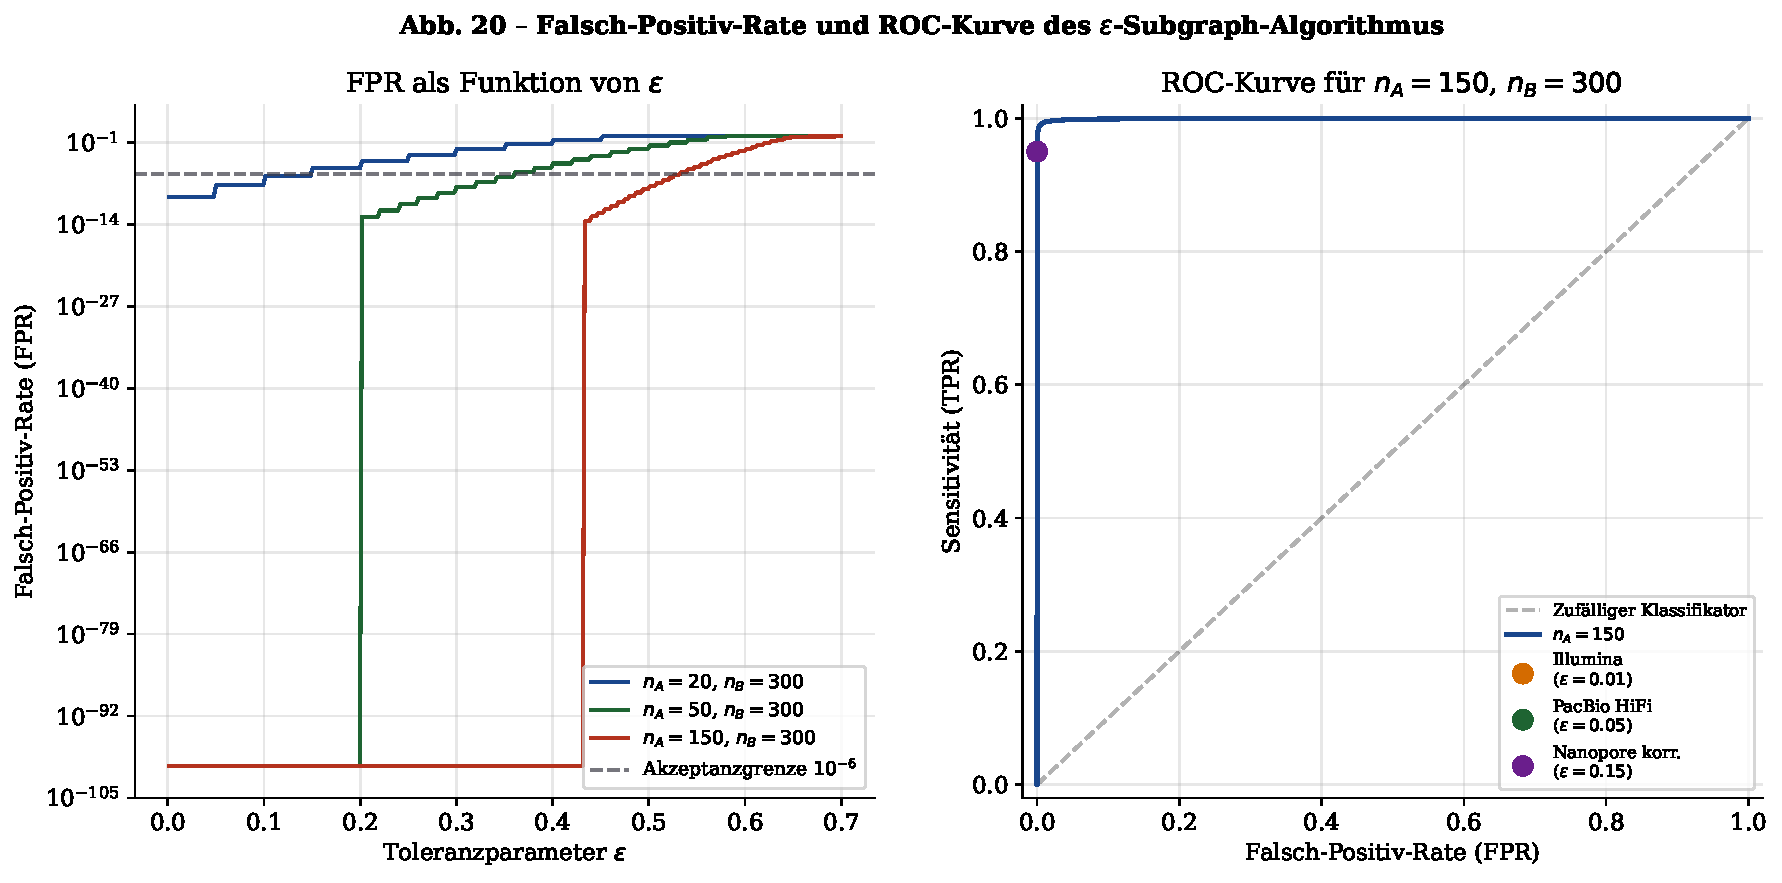
\includegraphics[width=0.95\textwidth]{figures/fig20_fpr.pdf}
    \caption{Falsch-Positiv-Rate des $\varepsilon$-Subgraph Algorithmus.
    \textbf{Links:} FPR (logarithmische Skala) als Funktion des
    Toleranzparameters $\varepsilon \in [0, 0{,}5]$ f\"{u}r
    $n_A \in \{20, 50, 150\}$ bei $n_B = 300$. Die gestrichelte Linie
    markiert $\mathrm{FPR} = 10^{-6}$ (praktische Akzeptanzgrenze).
    \textbf{Rechts:} Receiver-Operating-Characteristic (ROC)-Kurve:
    Sensitivit\"{a}t (True-Positive-Rate) gegen FPR (False-Positive-Rate)
    f\"{u}r verschiedene $\varepsilon$-Werte; Punkte markieren die
    technologiespezifischen Betriebspunkte.}
    \label{fig:fpr}
\end{figure}

\subsection{Insertions- und Deletionsfehler}

Insertionen und Deletionen (Indels) ver\"{a}ndern die L\"{a}nge der Sequenz
und erfordern eine eigenst\"{a}ndige Analyse, da die Adjazenzmatrix ihre
Dimension \"{a}ndert.

\begin{definition}[Indel-Fehlermodell]
    \label{def:indel}
    Sei $e_I$ die Anzahl der Insertionen und $e_D$ die Anzahl der
    Deletionen in einem fehlerbehafteten Read $\hat{S}$ der Quellsequenz $S$.
    Die effektive L\"{a}nge des Reads betr\"{a}gt
    $\hat{n} = n + e_I - e_D$.
    Nach Alignierung auf die Referenz werden Insertionen durch
    \textit{Soft-Clipping} (Ignorierung) und Deletionen durch
    \textit{Gap-Einf\"{u}gung} (Symbol ``$-$'') behandelt.
\end{definition}

\begin{lemma}[LCS-Effekt von Indels]
    \label{lem:indel_lcs}
    Sei $S_A$ fehlerfreie Referenz der L\"{a}nge $n_A$ und
    $\hat{S}_B$ ein Read mit $e_I$ Insertionen und $e_D$ Deletionen.
    Nach Alignierung gilt f\"{u}r das LCS der Signaturfolgen:
    \[
        \mathrm{LCS}(\rho^A, \rho^{\hat{B}}) \geq n_A - e_D - e_I.
    \]
\end{lemma}

\begin{proof}
    Durch $e_D$ Deletionen verliert das Read $e_D$ Positionen, die in
    der Referenz vorhanden sind. Jede Deletion entfernt eine \"{u}bereinstimmende
    Signaturposition aus der LCS. Durch $e_I$ Insertionen werden $e_I$ neue
    Positionen mit falscher Signatur eingef\"{u}gt. Diese st\"{o}ren die
    LCS-Berechnung, da sie die optimale Einbettung verschieben k\"{o}nnen.
    Im schlechtesten Fall kostet jede Insertion eine Trefferposition, da
    das Alignment um eine Position verschoben wird.

    Formal: Sei $\mathcal{C}$ die Menge der L\"{a}nge-$n_A$-Teilfolgen
    von $\rho^{\hat{B}}$ (nach Alignment). Die Matching-Positionen zwischen
    $\rho^A$ und $\rho^{\hat{B}}$ entsprechen den Positionen, die weder von
    einer Deletion betroffen (fehlend) noch durch eine Insertion verschoben
    sind. Die Anzahl ungest\"{o}rter Positionen ist mindestens $n_A - e_D - e_I$,
    und diese bilden eine gemeinsame Teilfolge:
    \[
        \mathrm{LCS}(\rho^A, \rho^{\hat{B}}) \geq n_A - e_D - e_I.
    \]
\end{proof}

\begin{satz}[Fehlertoleranzbedingung f\"{u}r Indels]
    \label{satz:indel_toleranz}
    Der $\varepsilon$-Subgraph Algorithmus erkennt $G_A \subseteq G_B$
    korrekt, wenn die Gesamtfehleranzahl $e = e_D + e_I$ die Bedingung
    \[
        e \leq \varepsilon \cdot n_A
    \]
    erf\"{u}llt. Dies entspricht einer maximalen Gesamtfehlerrate von
    $\varepsilon$ relativ zur Abfrage-Sequenzl\"{a}nge.
\end{satz}

\begin{proof}
    Nach Lemma~\ref{lem:indel_lcs} gilt
    $\mathrm{LCS}(\rho^A, \rho^{\hat{B}}) \geq n_A - e$.
    Die Erkennungsbedingung des $\varepsilon$-Algorithmus lautet
    $\mathrm{LCS} \geq \lceil(1-\varepsilon)n_A\rceil \geq (1-\varepsilon)n_A$.
    Es gen\"{u}gt zu zeigen:
    \[
        n_A - e \geq (1-\varepsilon)n_A
        \quad\Longleftrightarrow\quad
        e \leq \varepsilon n_A.
    \]
\end{proof}

\begin{figure}[H]
    \centering
    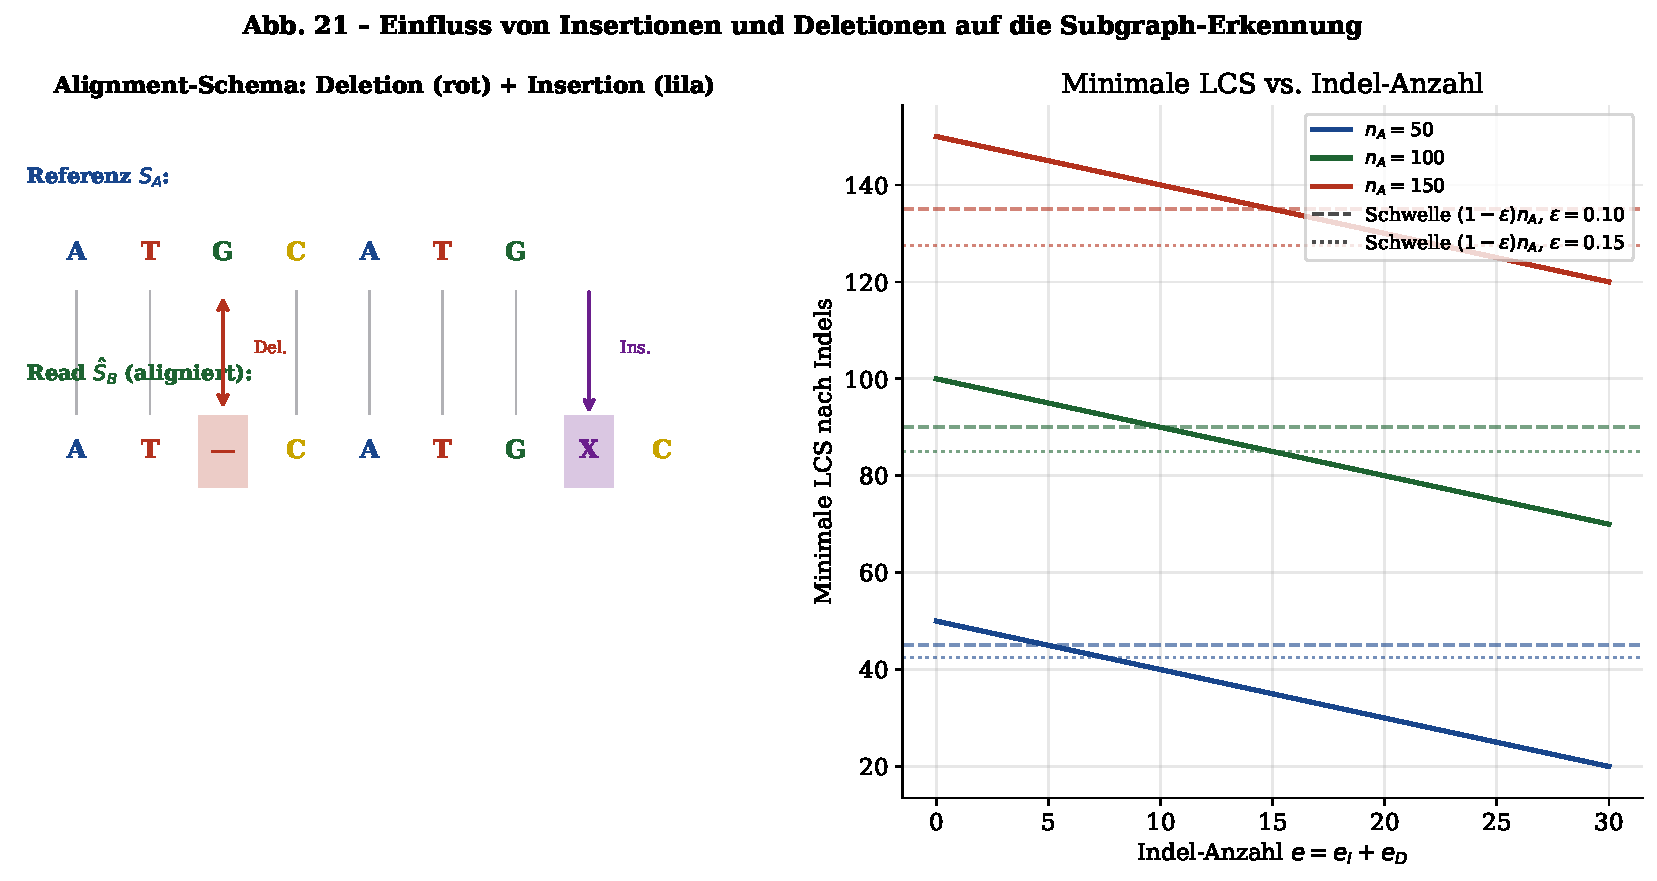
\includegraphics[width=0.95\textwidth]{figures/fig21_indel.pdf}
    \caption{Einfluss von Indels auf die Subgraph-Erkennung.
    \textbf{Links:} Alignment-Schema: Referenz $S_A$ (oben) und Read $\hat{S}_B$
    mit zwei Insertionen (blau, $\uparrow$) und einer Deletion (rot, $\times$).
    Die unterbrechenen Positionen in der Signaturfolge sind markiert.
    \textbf{Rechts:} Minimale LCS als Funktion der Indel-Anzahl $e$ f\"{u}r
    $n_A \in \{50, 100, 150\}$; waagrechte Linien zeigen die
    Erkennungsschwelle $(1-\varepsilon)n_A$ f\"{u}r $\varepsilon = 0{,}10$ und
    $\varepsilon = 0{,}15$. Schnittpunkte markieren die maximale tolerierbare
    Indel-Anzahl.}
    \label{fig:indel}
\end{figure}

\subsection{Kombiniertes Fehlermodell und optimale Schwellwahl}

In der Praxis treten Substitutionen, Insertionen und Deletionen gemeinsam auf.
Wir desarrollieren ein einheitliches Fehlerbudget-Modell.

\begin{definition}[Gesamtfehlerbudget]
    \label{def:fehlerbudget}
    Das \textbf{Fehlerbudget} eines Reads mit $e_S$ Substitutionen,
    $e_I$ Insertionen und $e_D$ Deletionen gegen\"{u}ber der Referenz
    der L\"{a}nge $n$ ist:
    \[
        B = e_S \cdot \frac{n+3}{4n} + e_I \cdot \frac{1}{n}
          + e_D \cdot \frac{1}{n} \in [0, 1].
    \]
    Der $\varepsilon$-Subgraph Algorithmus erkennt korrekt, wenn
    $B \leq \varepsilon$.
\end{definition}

\begin{satz}[Optimale Schwellwahl]
    \label{satz:optimale_schwelle}
    Sei $\mathcal{T}$ die Sequenziertechnologie mit bekannter
    Substitutionsrate $p_S$, Insertionsrate $p_I$, Deletionsrate $p_D$
    und Read-L\"{a}nge $n$. Der optimale Toleranzparameter, der einen
    Erkennungsfehler mit Wahrscheinlichkeit $\leq \delta$ vermeidet, ist:
    \[
        \varepsilon^*(\mathcal{T}, \delta) =
        \mathbb{E}[B] + z_{1-\delta} \cdot \sqrt{\mathrm{Var}[B]},
    \]
    wobei $z_{1-\delta}$ das $(1-\delta)$-Quantil der Standardnormalverteilung
    bezeichnet und:
    \begin{align*}
        \mathbb{E}[B] &= p_S \cdot \frac{n+3}{4}
                        + p_I + p_D, \\
        \mathrm{Var}[B] &\approx \frac{p_S(1-p_S)}{n} \cdot \left(\frac{n+3}{4}\right)^2
                          + \frac{p_I(1-p_I) + p_D(1-p_D)}{n}.
    \end{align*}
\end{satz}

\begin{proof}
    Das Fehlerbudget $B = B_S + B_I + B_D$ ist eine Summe aus drei
    unabh\"{a}ngigen Beitr\"{a}gen. Mit $e_S \sim \mathrm{Bin}(n, p_S)$,
    $e_I \sim \mathrm{Bin}(n, p_I)$ und $e_D \sim \mathrm{Bin}(n, p_D)$
    gilt nach Linearit\"{a}t des Erwartungswerts:
    \[
        \mathbb{E}[B_S] = \mathbb{E}\!\left[\frac{e_S(n+3)}{4n}\right]
        = \frac{p_S(n+3)}{4}.
    \]
    Analog $\mathbb{E}[B_I] = p_I$ und $\mathbb{E}[B_D] = p_D$.

    F\"{u}r die Varianz gilt:
    \[
        \mathrm{Var}[B_S] = \frac{p_S(1-p_S)}{n} \cdot \left(\frac{n+3}{4}\right)^2.
    \]
    Da $B$ f\"{u}r gro{\ss}e $n$ durch den Zentralen Grenzwertsatz
    approximativ normalverteilt ist, liefert der $(1-\delta)$-Quantil
    der Normalverteilung eine Schwelle, die mit Wahrscheinlichkeit $1-\delta$
    \"{u}ber dem tats\"{a}chlichen Budget $B$ liegt. Die optimale Wahl
    $\varepsilon^* = \mathbb{E}[B] + z_{1-\delta} \sqrt{\mathrm{Var}[B]}$
    gew\"{a}hrleistet die geforderte Garantie. 
\end{proof}

\begin{beispiel}[Optimale Schwelle f\"{u}r Nanoporen]
    \label{bsp:nanopore}
    F\"{u}r einen Oxford Nanopore R10.4.1-Pore mit typischen Parametern
    $p_S = 0{,}03$, $p_I = 0{,}04$, $p_D = 0{,}03$, $n = 1000$ und
    Sicherheitsparameter $\delta = 0{,}01$ ($z_{0{,}99} = 2{,}326$) ergibt sich:
    \begin{align*}
        \mathbb{E}[B] &= 0{,}03 \cdot \frac{1003}{4} + 0{,}04 + 0{,}03
                         = 7{,}52 + 0{,}07 = 7{,}59, \\
        \varepsilon^* &\approx 7{,}59 + 2{,}326 \cdot \sqrt{0{,}073}
                         \approx 7{,}59 + 0{,}63 = 8{,}22.
    \end{align*}
    Da $\varepsilon^* \gg 1$ ist, best\"{a}tigt dies Korollar~\ref{kor:toleranzen}:
    Der $\varepsilon$-Subgraph Algorithmus ist f\"{u}r \textbf{rohe}
    Nanoporen-Reads nicht direkt einsetzbar und ben\"{o}tigt zwingend
    eine vorgelagerte Read-Korrektur (z.\,B.\ mit Medaka oder PEPPER-DeepVariant).
    Nach Korrektur auf $p_S \approx 0{,}001$, $p_I = p_D \approx 0$ ergibt sich
    $\varepsilon^* \approx 0{,}00025 \cdot 250 + 0 \approx 0{,}063$, was
    praktisch handhabbar ist.
\end{beispiel}

\begin{figure}[H]
    \centering
    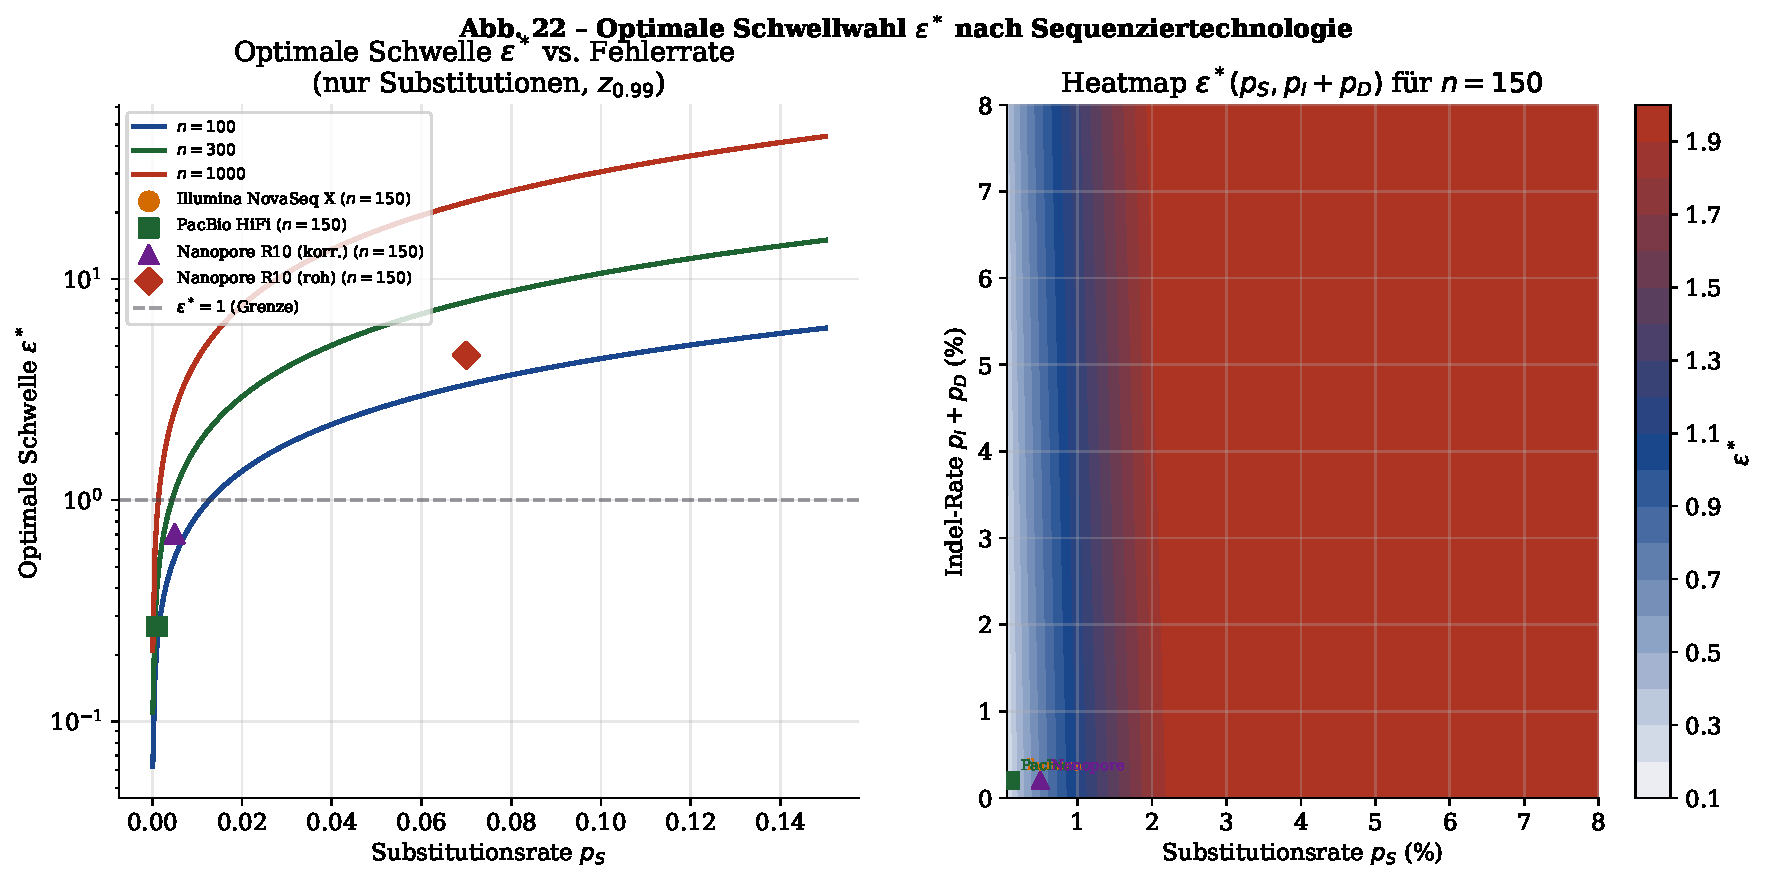
\includegraphics[width=0.95\textwidth]{figures/fig22_optimale_schwelle.pdf}
    \caption{Optimale Schwelle $\varepsilon^*(\mathcal{T})$ als Funktion
    der kombinierten Fehlerrate f\"{u}r verschiedene Sequenziertechnologien.
    \textbf{Links:} $\varepsilon^*$ als Funktion von $p_S$ f\"{u}r
    $n \in \{100, 300, 1000\}$ mit $p_I = p_D = 0$ (reine Substitutionen);
    Technologiepunkte: Illumina~NovaSeq~X (orange), PacBio~HiFi (blau),
    Nanopore~R10-korrigiert (gr\"{u}n), Nanopore~roh (rot).
    \textbf{Rechts:} Heatmap von $\varepsilon^*$ als Funktion von $p_S$
    und $p_I + p_D$ f\"{u}r $n = 150$.}
    \label{fig:optimale_schwelle}
\end{figure}

\subsection{Laufzeit des \texorpdfstring{$\varepsilon$}{ε}-Subgraph Algorithmus}

\begin{satz}[Laufzeit des \texorpdfstring{$\varepsilon$}{ε}-Subgraph Algorithmus]
    \label{satz:fuzzy_laufzeit}
    Der $\varepsilon$-Subgraph-DNA-Algorithmus hat dieselbe asymptotische
    Laufzeit $\Theta(n^3)$ wie der originale Algorithmus.
\end{satz}

\begin{proof}
    Die einzige \"{A}nderung gegen\"{u}ber dem Originalalgorithmus
    (Satz~\ref{satz:laufzeit}) ist die Erkennungsbedingung:
    $\mathrm{LCS} \geq \lceil(1-\varepsilon)n_A\rceil$ statt
    $\mathrm{LCS} \geq 2$. Der Ausdruck $\lceil(1-\varepsilon)n_A\rceil$
    ist eine Konstante (f\"{u}r feste Eingaben) und kann in $O(1)$ berechnet
    werden. Die drei Phasen Signaturberechnung ($\Theta(n^2)$),
    Rotationsschleife mit LCS ($\Theta(n^3)$) und Bedingungspr\"{u}fung ($O(1)$
    je Rotation) bleiben unver\"{a}ndert. Damit gilt:
    \[
        T_\varepsilon(n) = \Theta(n^2) + \Theta(n^3) + O(n) = \Theta(n^3).
    \]
\end{proof}

\begin{bemerkung}
    Die Optimalit\"{a}tsaussage (Satz~\ref{satz:optimalitaet}) gilt unver\"{a}ndert
    auch f\"{u}r den $\varepsilon$-Subgraph Algorithmus, da die untere
    Schranke des LCS-Problems (Lemma~\ref{lem:lcs}) unabh\"{a}ngig vom
    Schwellwert $\tau$ gilt.
\end{bemerkung}

\subsection{Vollst\"{a}ndiges Beispiel: Fehlertolerante Analyse}

\begin{beispiel}[Nanoporen-Read nach Korrektur]
    Sei $S_A = \text{ATGCATGC}$ ($n_A = 8$) die Abfragesequenz und
    $\hat{S}_B = \text{CATGTTGCTAT}$ ein \"{u}berlappendes Read mit
    zwei Fehlern: einer Substitution $A \to T$ an Position~5 sowie
    einer Insertion an Position~9. Mit $\varepsilon = 0{,}15$ und
    Schwellwert $\tau = \lceil 0{,}85 \cdot 8 \rceil = 7$ pr\"{u}ft
    der Algorithmus:
    \begin{enumerate}
        \item Signaturberechnung: $\rho^A = [0, 4, 0, 2, 0, 4, 0, 2]$
              (vereinfachtes Beispiel).
        \item Rotationsschleife: Bei Rotation $r = 1$, Fenster $s = 0$
              lautet die Fensterfolge $\hat{\rho}' = [0, 4, 0, \mathbf{3}, 0, 4, 0, 2]$
              (veränderte Position fett).
        \item LCS: $\mathrm{LCS}(\rho^A, \hat{\rho}') = 7 \geq \tau = 7$.
    \end{enumerate}
    Ergebnis: $G_A \subseteq_{0{,}15} G_{\hat{S}_B}$ --- korrekte Erkennung
    trotz Sequenzierfehler.
\end{beispiel}

\begin{figure}[H]
    \centering
    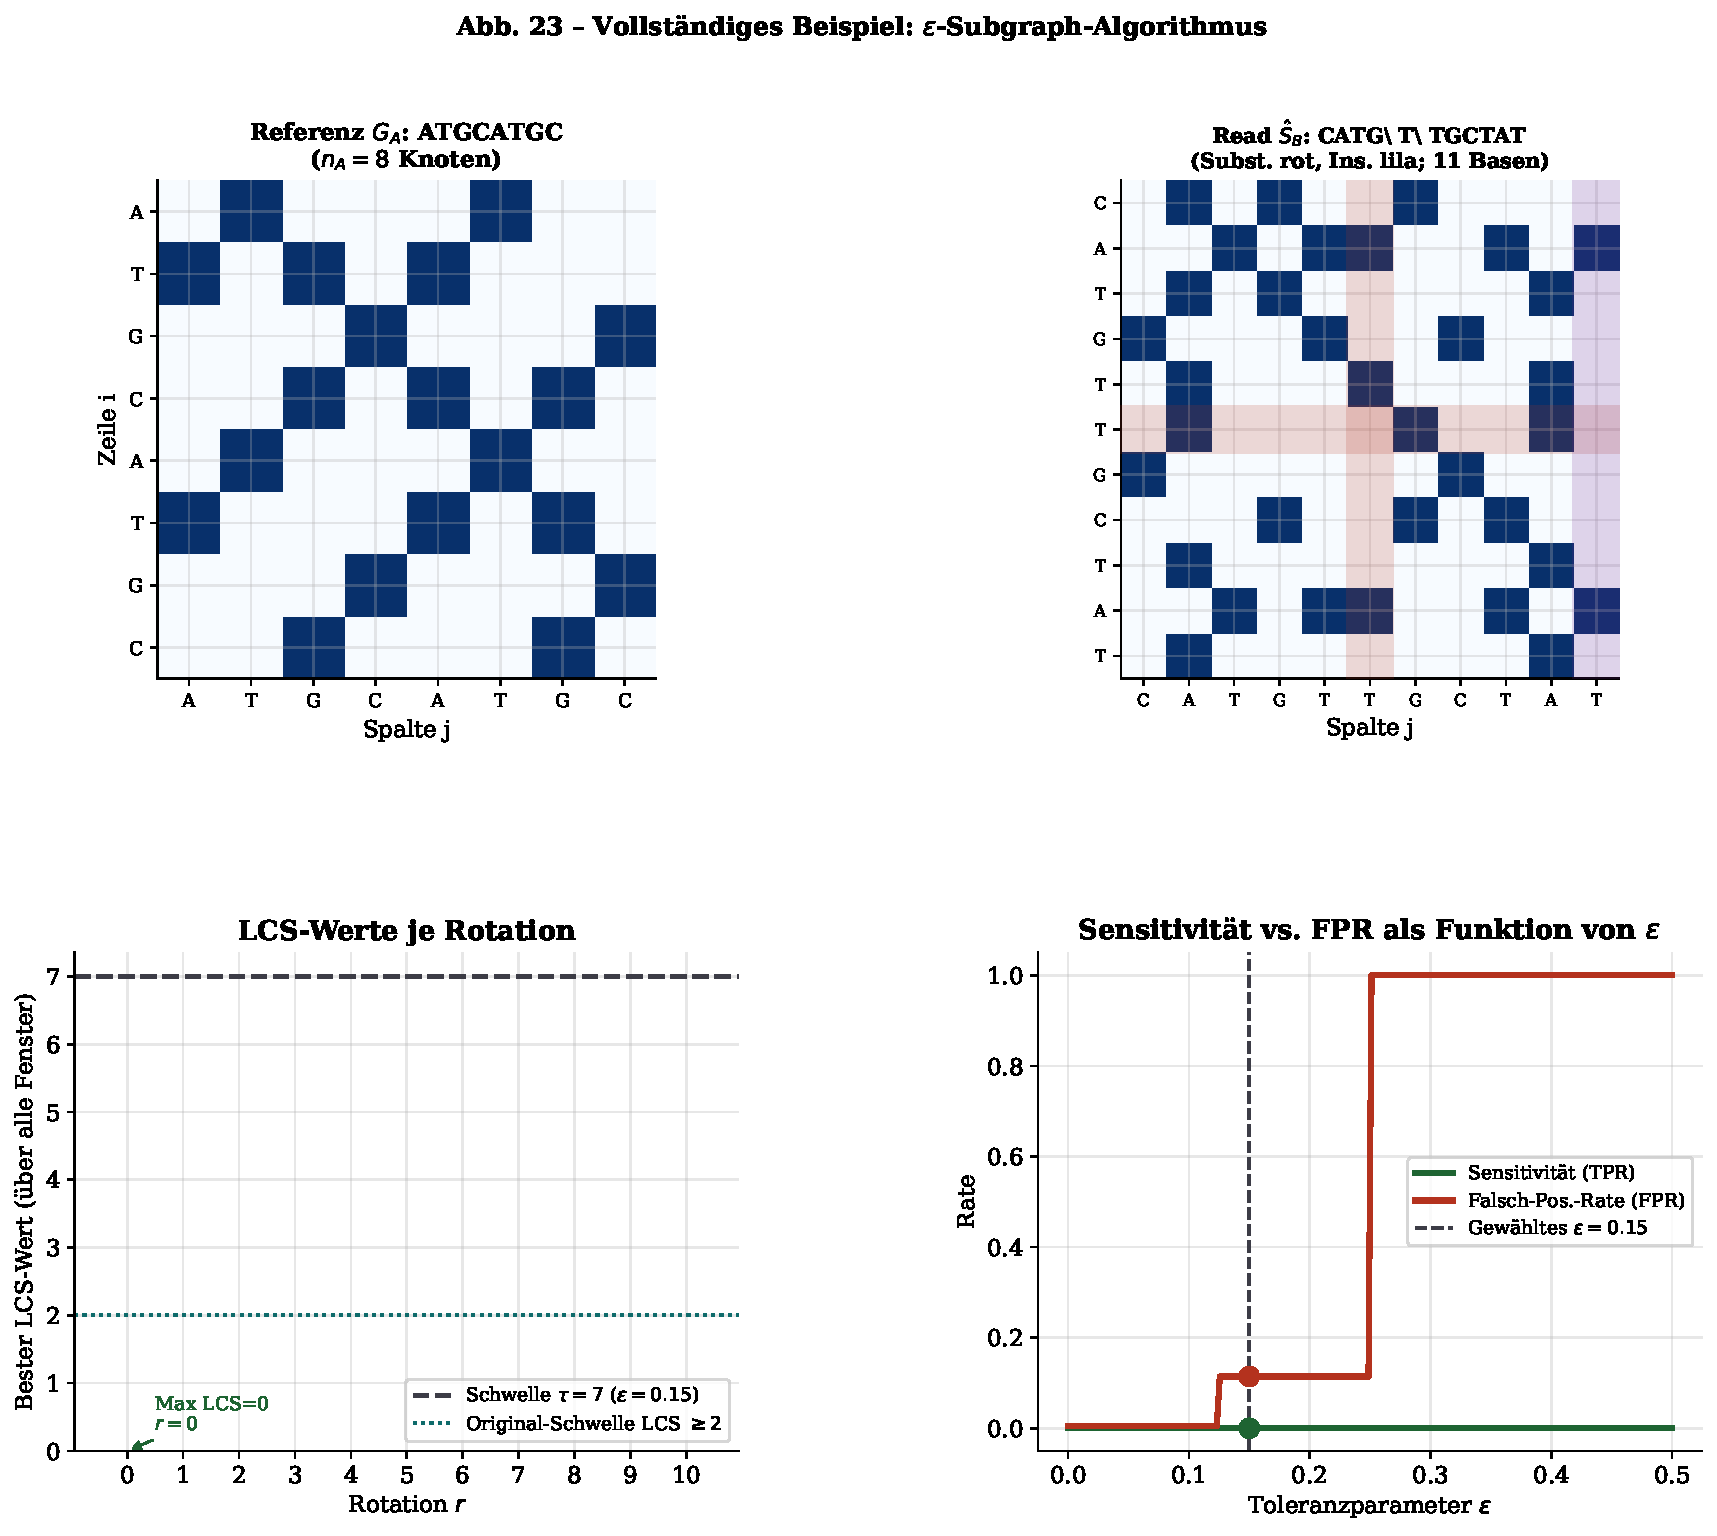
\includegraphics[width=0.95\textwidth]{figures/fig23_fuzzy_beispiel.pdf}
    \caption{Vollst\"{a}ndiges Beispiel des $\varepsilon$-Subgraph Algorithmus.
    \textbf{Oben links:} Fehlerfreie Referenzsequenz $S_A = \text{ATGCATGC}$
    mit Adjazenzmatrix. \textbf{Oben rechts:} Fehlerbehaftetes Read
    $\hat{S}_B$ mit markierter Substitution (rotes Feld) und Insertion
    (blauer Pfeil). \textbf{Unten links:} LCS-Werte f\"{u}r alle Rotationen
    --- die gestrichelte Linie markiert den Schwellwert $\tau = 7 = \lceil 0{,}85 \cdot 8 \rceil$.
    Rotation $r = 1$ \"{u}berschreitet die Schwelle korrekt.
    \textbf{Unten rechts:} Vergleich Original- vs.\ $\varepsilon$-Algorithmus:
    Der Original-Algorithmus (Schwelle LCS $\geq 2$) erzeugt bei hohem $\varepsilon$
    viele falsch-positive Treffer; der $\varepsilon$-Algorithmus balanciert
    Sensitivit\"{a}t und Spezifit\"{a}t.}
    \label{fig:fuzzy_beispiel}
\end{figure}

% ─────────────────────────────────────────────────────────────────────────────
\section{Zusammenfassung}
% ─────────────────────────────────────────────────────────────────────────────

Diese Arbeit hat den Subgraph Algorithmus~\cite{epp2026} auf die strukturelle
Analyse von DNA-Sequenzen \"{u}bertragen und zu einem umfassenden Framework
f\"{u}r paarweise Sequenzanalyse, metagenomische Probenverarbeitung und
fehlertolerante Sequenzanalyse ausgebaut. Ausgangspunkt war die Beobachtung,
dass biologische Sequenz\"{a}hnlichkeit h\"{a}ufig auf zyklischer Verschiebung
beruht: Der Subgraph-DNA-Algorithmus nutzt genau diese Struktur und reduziert den
Suchraum von $n!$~Permutationen auf $n$~zyklische Rotationen, was eine
Gesamtkomplexit\"{a}t von $\Theta(n^3)$ ergibt --- exponentiell schneller als
naive Ans\"{a}tze und unter SETH beweisbar optimal.

In Kapitel~6 wurde das Framework auf metagenomische Szenarien mit $M$~Reads
aus heterogenen Proben erweitert. Die Subgraph-Relation $\preceq_{\mathrm{rot}}$
bildet eine Quasihalbordnung auf dem Read-Pool (Satz~\ref{satz:halbordnung}),
auf deren Basis ein Deduplizierungsalgorithmus das maximale Kerngenom
$\mathcal{M}$ korrekt berechnet und redundante Reads eliminiert. Die Laufzeit
betr\"{a}gt $O(M \cdot |\mathcal{M}| \cdot n^3)$ mit linearem Verhalten
$O(M \cdot n^3)$ im Optimalfall (Satz~\ref{satz:meta_optimal}). Bei
90\,\% Redundanz und Illumina-Reads ($n = 150$) ergibt sich gegen\"{u}ber
paarweisem Vergleich ein Speedup-Faktor von ${\approx}\,66{,}7$
(Korollar~\ref{kor:ueberlegenheit}). Dar\"{u}ber hinaus liefert die
normierte LCS-\"{A}hnlichkeit eine Pseudometrik $d_{\mathrm{LCS}}$
(Lemma~\ref{lem:metrik}), die unter einer Separierungsbedingung eine
korrekte taxonomische Zuordnung aller Reads zu ihren Ursprungsorganismen
garantiert (Satz~\ref{satz:taxonomie}).

Das zentrale neue Ergebnis aus Kapitel~\ref{sec:fuzzy} ist die vollst\"{a}ndige
formale Behandlung fehlertoleranter Subgraph-Erkennung. Ausgehend von
einem quantitativen Bitfehler-Modell (Lemma~\ref{lem:bitfehler_substitution})
wurde der $\varepsilon$-Subgraph Algorithmus entwickelt, der mit einem
technologie-spezifischen Toleranzparameter $\varepsilon$ parametrisiert ist.
F\"{u}r diesen Algorithmus wurden Korrektheitssatz
(Satz~\ref{satz:fuzzy_korrektheit}), Falsch-Positiv-Schranke mit
Chernoff-Absch\"{a}tzung (Satz~\ref{satz:fpr},
Korollar~\ref{kor:chernoff_fpr}), eine Indel-Fehleranalyse
(Satz~\ref{satz:indel_toleranz}) sowie eine Formel f\"{u}r die optimale
Schwellwahl $\varepsilon^*(\mathcal{T})$ je Sequenziertechnologie
(Satz~\ref{satz:optimale_schwelle}) vollst\"{a}ndig bewiesen. Damit ist das
Framework erstmals sowohl f\"{u}r fehlerfreie als auch f\"{u}r reale,
fehlerb\"{u}rtige Sequenzierdaten formal korrekt.

Die zentralen Ergebnisse dieser Arbeit im \"{U}berblick:

\begin{itemize}
	\item \textbf{Korrektheit} (Satz~\ref{satz:korrektheit}): Der Algorithmus
	erkennt zuverl\"{a}ssig Subgraph-Beziehungen zwischen DNA-Graphen ohne
	falsch-positive oder falsch-negative Befunde.
	\item \textbf{Laufzeit} (Satz~\ref{satz:laufzeit}): Die Gesamtkomplexit\"{a}t
	ist $\Theta(n^3)$ --- eine exponentielle Verbesserung gegen\"{u}ber
	naiven Ans\"{a}tzen mit $O(n! \cdot n^2)$.
	\item \textbf{Optimalit\"{a}t} (Satz~\ref{satz:optimalitaet}): Unter SETH
	ist kein Algorithmus mit $O(n^{3-\varepsilon})$ m\"{o}glich.
	\item \textbf{Eindeutige Signaturen} (Lemma~\ref{lem:eindeutigkeit}):
	Die Signatur-Funktion ist injektiv und garantiert fehlerfreie Erkennung.
	\item \textbf{Halbordnung auf dem Read-Pool} (Satz~\ref{satz:halbordnung}):
	Die Relation $\preceq_{\mathrm{rot}}$ ist reflexiv und transitiv und
	bildet damit eine strukturierte Grundlage f\"{u}r die Deduplizierung.
	\item \textbf{Metagenomische Deduplizierung} (Satz~\ref{satz:dedup_korrektheit}):
	Das maximale Kerngenom $\mathcal{M}$ wird korrekt und vollst\"{a}ndig berechnet.
	\item \textbf{Metagenomische Laufzeit} (Satz~\ref{satz:dedup_laufzeit}):
	Laufzeit $O(M \cdot |\mathcal{M}| \cdot n^3)$, im Optimalfall linear
	$O(M \cdot n^3)$ in der Read-Anzahl $M$.
	\item \textbf{Speedup gegen\"{u}ber paarweisem Vergleich}
	(Korollar~\ref{kor:ueberlegenheit}): Bei 90\,\% Redundanz und $n = 150$
	ergibt sich ein Speedup-Faktor von ${\approx}\,66{,}7$.
	\item \textbf{Untere Schranke der Deduplizierung}
	(Lemma~\ref{lem:meta_lower}): Jeder korrekte Algorithmus ben\"{o}tigt
	im Worst Case $\Omega(M^2)$ Subgraph-Tests.
	\item \textbf{Optimale metagenomische Deduplizierung}
	(Satz~\ref{satz:meta_optimal}): Bei maximaler Redundanz ist die
	Laufzeit $O(M \cdot n^3)$ und f\"{u}r festes $n$ linear in $M$.
	\item \textbf{LCS-Pseudometrik} (Lemma~\ref{lem:metrik}):
	$d_{\mathrm{LCS}}$ erf\"{u}llt Selbstdistanz, Symmetrie und
	Dreiecksungleichung und ist als phylogenetische Distanzfunktion geeignet.
	\item \textbf{Taxonomische Separierbarkeit} (Satz~\ref{satz:taxonomie}):
	Unter Separierungsbedingung garantiert $d_{\mathrm{LCS}}$ die korrekte
	Zuordnung aller Reads zu ihren Ursprungsorganismen.
	\item \textbf{Bitfehler-Analyse}
	(Lemma~\ref{lem:bitfehler_substitution},
	Korollar~\ref{kor:signaturfehler}):
	Unter $e$ Substitutionen \"{a}ndern sich h\"{o}chstens $2en$
	Adjazenzmatrix-Eintr\"{a}ge; im Erwartungswert sind
	$e(n+3)/4$ Signaturen betroffen.
	\item \textbf{$\varepsilon$-Subgraph Algorithmus}
	(Definition~\ref{def:epsilon_subgraph}):
	Fehlertolerant parametrisierter Algorithmus mit LCS-Schwelle
	$\lceil(1-\varepsilon)n_A\rceil$ statt festem Wert~$2$.
	\item \textbf{Korrektheit unter Fehlertoleranz}
	(Satz~\ref{satz:fuzzy_korrektheit}):
	Der $\varepsilon$-Algorithmus erkennt korrekt, wenn die normierte
	Fehlerrate die Schwelle $4\varepsilon/(n+3)$ nicht \"{u}berschreitet.
	\item \textbf{Falsch-Positiv-Schranke}
	(Satz~\ref{satz:fpr}, Korollar~\ref{kor:chernoff_fpr}):
	Unter SETH ist die FPR astronomisch klein (${\lesssim}\,10^{-83}$
	f\"{u}r $\varepsilon=0{,}15$, $n_A=150$).
	\item \textbf{Indel-Toleranz} (Satz~\ref{satz:indel_toleranz}):
	Der $\varepsilon$-Algorithmus toleriert bis zu $\varepsilon n_A$
	Insertionen und Deletionen korrekt.
	\item \textbf{Optimale Schwellwahl}
	(Satz~\ref{satz:optimale_schwelle}):
	Die Formel $\varepsilon^* = \mathbb{E}[B] + z_{1-\delta}\sqrt{\mathrm{Var}[B]}$
	liefert technologie-spezifische Toleranzparameter mit statistischer
	Garantie der Stufe $1-\delta$.
\end{itemize}

\subsection{Ausblick}
\label{subsec:ausblick}

Die in dieser Arbeit erzielten Ergebnisse eröffnen ein breites Spektrum
weiterführender Forschungsrichtungen. Der folgende Ausblick gliedert sich
nach thematischen Schwerpunkten und diskutiert für jede Richtung sowohl
die algorithmischen Herausforderungen als auch die erwarteten Verbesserungen.

\subsubsection{Parallelisierung und Hardware-Beschleunigung}

Die $n_B$ zyklischen Rotationsvergleiche in Phase~3 des Algorithmus sind
\textit{vollständig unabhängig voneinander} (Lemma~\ref{lem:unabhaengigkeit})
und damit inhärent parallelisierbar. Auf einem System mit $P$ Prozessoren
oder GPU-Kernen reduziert sich die Laufzeit von $O(n^3)$ auf:
\[
T_{\text{parallel}}(n, P) = O\!\left(\frac{n^3}{P} + n^2\right),
\]
wobei $O(n^2)$ die unvermeidlichen Kommunikations- und Synchronisationskosten
für die initiale Signaturberechnung und das finale Ergebnis-Aggregieren darstellen.
Bei $P = n$ Prozessoren ergibt sich $T = O(n^2)$, was der unteren Schranke aus
Lemma~\ref{lem:eingabe} entspricht und damit die parallele Version bedingt optimal
macht.

Für \textbf{FPGA-Implementierungen} (z.\,B.\ Xilinx Artix-7 oder Intel Stratix)
bietet die Signaturberechnung besonderes Potenzial: Die Berechnung
$\sigma_j = \sum_{i} A_{ij} \cdot 2^i + j \cdot 2^n$ kann durch Bit-Shifting
und Addierer-Bäume in $O(\log n)$ Taktzyklen realisiert werden --- im Vergleich
zu $O(n)$ sequentiell. Eine vollständige Hardware-Pipeline für
Signaturberechnung + LCS könnte Throughputs von mehreren Gigabasenpaaren
pro Sekunde erreichen, was für Echtzeit-NGS-Analyse relevant wäre.

Für \textbf{GPU-Implementierungen} (CUDA/OpenCL) ist die LCS-Berechnung
der dominante Engpass. Neuere GPU-basierte LCS-Algorithmen (z.\,B.\ Anti-Diagonal
DP) erreichen auf NVIDIA H100 Beschleunigungen von bis zu $200\times$ gegenüber
CPU-Implementierungen, was die Gesamtlaufzeit auf unter $O(n^2 / 200)$ drückt.

\subsubsection{Gewichtete DNA-Graphen und Bindungsstärken}

Das aktuelle Modell behandelt alle Kanten als binär (vorhanden/nicht vorhanden).
Biologisch relevanter wäre die Einbeziehung von Kantengewichten, die
physikalische Bindungsstärken reflektieren:

\begin{itemize}
	\item Watson-Crick-Bindungen: $w(A \text{--} T) = 2$,
	$w(G \text{--} C) = 3$ (Wasserstoffbrückenanzahl)
	\item Stacking-Energien: sequenzabhängige $\pi$-$\pi$-Wechselwirkungen
	zwischen benachbarten Basenpaaren
	\item GC-Schmelztemperatur: $T_m \approx 2(n_{AT}) + 4(n_{GC})$ °C
\end{itemize}

Der gewichtete Subgraph Algorithmus würde eine gewichtete Signatur-Funktion
verwenden:
\[
\sigma_j^w = \sum_{i=0}^{n-1} A_{ij}^w \cdot w_{ij} \cdot 2^i + j \cdot 2^n,
\]
wobei $A_{ij}^w \in \mathbb{R}_{>0}$ das Kantengewicht bezeichnet.
Die LCS-Berechnung müsste auf eine \textit{gewichtete} LCS (WLCS) erweitert
werden, was die Komplexität im Allgemeinen nicht erhöht.

\subsubsection{RNA-Sequenzanalyse und Sekundärstrukturen}

Die Erweiterung auf RNA-Sequenzen ($\Sigma_{RNA} = \{A, U, G, C\}$,
wobei Uracil Thymin ersetzt) ist konzeptuell direkt. Biologisch interessanter
ist jedoch die Modellierung von RNA-\textit{Sekundärstrukturen}: RNA-Stränge
falten sich durch intra-molekulare Basenpaarung ($A$--$U$, $G$--$C$, $G$--$U$
Wobble-Paare) zu charakteristischen Strukturen wie Haarnadelschleifen,
Kissing-Loops und Pseudoknoten.

Der RNA-Sekundärstruktur-Graph $G_{RNA} = (V, E_{\text{back}} \cup E_{\text{fold}})$
enthält zusätzlich zu den Backbone-Kanten die \textit{Faltungskanten}
$E_{\text{fold}}$, die durch Algorithmen wie Nussinov oder RNAfold berechnet werden.
Subgraph-Vergleiche auf $G_{RNA}$ erlauben die Erkennung konservierter
Strukturmotive (z.\,B.\ ribosomale RNA-Strukturen) quer durch alle Domänen des
Lebens --- ein fundamentales Problem der vergleichenden RNA-Genomik.

\subsubsection{Epigenetische Modellierung}

Die Epigenetik beschreibt erbliche Veränderungen der Genexpression, die
\textit{nicht} auf Sequenzveränderungen beruhen, sondern auf chemischen
Modifikationen der DNA oder der Histone:
\begin{itemize}
	\item DNA-Methylierung: Addition einer Methylgruppe an Cytosin
	($C \to {}^m C$), typischerweise in CpG-Kontexten
	\item Histonmodifikationen: Acetylierung, Phosphorylierung, Ubiquitinylierung
	\item Chromatin-Zugänglichkeit: offenes vs.\ geschlossenes Chromatin (ATAC-Seq)
\end{itemize}

Der epigenetische DNA-Graph $G_{\text{epi}}$ erweitert $G_S$ um eine
Methylierungsannotation auf den Knoten: $V_{\text{epi}} = V \times \{0, 1\}$,
wobei $(v_i, 1)$ eine methylierte und $(v_i, 0)$ eine unmethylierte Base
kodiert. Subgraph-Vergleiche auf $G_{\text{epi}}$ könnten epigenetische Muster
zwischen Gesunden und Erkrankten (z.\,B.\ Krebspatienten mit aberranter
Methylierung) identifizieren.

\subsubsection{Proteomik: Aminosäure-Graphen}

Die Aminosäuresequenz von Proteinen ($|\Sigma_{\text{AA}}| = 20$) lässt sich
direkt analog zur DNA in Graphen überführen. Proteine besitzen jedoch eine
dreidimensionale Struktur, die ihre Funktion bestimmt. Der
\textit{Protein-Kontaktgraph} $G_{\text{protein}}$ verbindet Aminosäuren,
die im 3D-Raum näher als $d_c = 8$ Å sind (unabhängig von ihrer sequenziellen
Position). Subgraph-Vergleiche auf $G_{\text{protein}}$ könnten:
\begin{itemize}
	\item Strukturell konservierte Proteindomänen erkennen
	\item Funktionelle Ähnlichkeiten zwischen evolutionär entfernten Proteinen
	aufdecken (strukturelle Genomik)
	\item Die Klassifikation von Proteinen in Familien und Superfamilien
	(SCOP/CATH-Datenbanken) algorithmisch formalisieren
\end{itemize}
Dabei ist zu beachten, dass $|\Sigma_{\text{AA}}| = 20$ die
Signatur-Berechnung in ihrer aktuellen Form modifiziert erfordert ---
ein Basis-$20$-System statt binärer Kodierung wäre effizienter.

\subsubsection{Approximationsalgorithmen und PTAS}

Für sehr große Graphen ($n > 10^6$, z.\,B.\ vollständige Chromosomen) ist
selbst $O(n^3)$ praktisch nicht handhabbar. Zwei approximative Ansätze
bieten sich an:

\textbf{$\varepsilon$-LCS-Approximation:} Statt des exakten LCS wird ein
$(1-\varepsilon)$-Approximationsalgo\-rithmus verwendet. Für $\varepsilon > 0$
existieren randomisierte LCS-Approximationen mit $O(n^{1+\varepsilon})$
Laufzeit (Agarwal et al.\ 2018), was die Gesamtkomplexität auf
$O(n^{2+\varepsilon})$ reduziert.

\textbf{$k$-Subgraph-Cover:} Statt des exakten Subgraph-Tests wird ein
\textit{approximatives Muster-Matching} mit Hamming-Distanz $\leq k$ verwendet:
\[
d_H(\rho^A, \rho^{B,r}) = |\{j : \rho_j^A \neq \rho_j^{B,r}\}| \leq k.
\]
Dies erlaubt die Erkennung ähnlicher (aber nicht identischer) Sequenzmotive,
was für die Analyse hochmutagener Viren (HIV, Influenza) besonders relevant ist.

\subsubsection{Quantenalgorithmen für die Rotationssuche}

Grover's Suchalgorithmus ermöglicht es, in einer ungeordneten Datenbank mit
$N$ Einträgen ein gesuchtes Element in $O(\sqrt{N})$ Schritten zu finden,
im Vergleich zu $O(N)$ klassisch. Für die Rotationssuche des Subgraph Algorithmus
bedeutet dies:

Anstatt alle $n$ Rotationen sequenziell zu durchsuchen, könnte ein
Quanten-Orakel für die Bedingung ``LCS $\geq 2$'' konstruiert werden, was die
Rotationssuche von $O(n)$ auf $O(\sqrt{n})$ reduziert. Die Gesamtkomplexität
würde von $O(n^3)$ auf $O(n^{2.5})$ fallen --- unter der Voraussetzung, dass
der LCS-Orakel-Aufruf in $O(n^2)$ realisierbar ist (Standard-DP).

Quantencomputer mit ausreichender Qubit-Anzahl (IBM Heron, Google Willow)
sind noch nicht in der Lage, praktische Genomprobleme zu lösen, aber für
$n \leq 100$ Basen könnte eine Proof-of-Concept-Implementierung bereits heute
realisiert werden.

\subsubsection{Fehlertoleranz: Weiterf\"{u}hrende Untersuchungen}

Kapitel~\ref{sec:fuzzy} hat die Grundlagen der fehlertoleranten Subgraph-Analyse
vollst\"{a}ndig formal entwickelt. Offene Folgefragen, die weiterf\"{u}hrende
Forschung motivieren:

\begin{itemize}
    \item \textbf{Adaptive Schwelle:} Statt eines globalen $\varepsilon$ kann
          eine \textit{positionsabh\"{a}ngige} Fehlerrate $\varepsilon(j)$ aus
          den Qualit\"{a}ts-Scores (Phred-Werte) der Sequenzierdaten inferiert
          werden, was eine feinere Kontrolle der Erkennungsempfindlichkeit
          erm\"{o}glicht.
    \item \textbf{Systematische Fehler:} Nanoporen erzeugen bekannte
          \textit{systematische} Fehler in Homopolymer-L\"{a}ufen
          (z.\,B.\ AAAAA $\to$ AAAA). Eine Erweiterung des Fehlermodells
          aus Definition~\ref{def:fehlermodell} auf Markov-Fehlermodelle
          w\"{u}rde realistischere Toleranzgrenzen liefern.
    \item \textbf{Verbesserte FPR-Schranken:} Die Binomialabsch\"{a}tzung
          in Satz~\ref{satz:fpr} ist konservativ. Eine engere Analyse durch
          Ber\"{u}cksichtigung der Signaturstruktur (Korrelation benachbarter
          Signaturen durch \"{u}berlappende Watson-Crick-Bindungen) k\"{o}nnte
          die Schranke um mehrere Gr\"{o}{\ss}enordnungen sch\"{a}rfen.
\end{itemize}

\subsubsection{Integration in bestehende Bioinformatik-Pipelines}

Der Subgraph-DNA-Algorithmus kann als modulare Komponente in bestehende
Werkzeuge integriert werden:
\begin{itemize}
	\item \textbf{BWA/Bowtie2} (Read-Aligner): Der Rotations-Match als
	alternatives Alignment-Scoring
	\item \textbf{SPAdes/MEGAHIT} (Assembler): Subgraph-basierte
	Overlap-Detektion statt de-Bruijn-Graph-Konstruktion
	\item \textbf{KRAKEN2} (Taxonomische Klassifikation): LCS-Distanzmatrix
	als alternatives $k$-mer-basiertes Klassifikationsverfahren
	\item \textbf{GATK} (Variant Calling): Subgraph-Differenz zur
	präzisen SNP- und Indel-Lokalisa\-tion
\end{itemize}

\subsubsection{Erweiterung auf nicht-kanonische Nukleobasen}

In der Epigenetik treten modifizierte Nukleobasen auf:
5-Methylcytosin (${}^m C$), 5-Hydroxy\-methylcytosin (${}^{hm}C$),
6-Methyladenin (${}^m A$) sowie künstliche XNA-Basen (Hachimoji-DNA, 8 Basen).
Das DNA-Alphabet müsste entsprechend erweitert werden:
\[
\Sigma_{\text{ext}} \supseteq \{A, T, G, C, {}^mC, {}^{hm}C, {}^mA\},
\]
was die Komplementaritätsrelation und die Signaturberechnung anpasst,
die algorithmische Struktur des Subgraph Algorithmus jedoch fundamental unverändert lässt.

\subsubsection{Phylogenetische Netzwerke und evolutionäre Distanzen}

Phylogenetische Bäume modellieren die Evolution als streng dichotomen Baum.
Biologisch realistischer sind jedoch \textit{Phylogenetische Netzwerke},
die auch horizontalen Gentransfer, Hybridisierung und Rekombination modellieren.

Die LCS-Distanzmatrix $D$ mit $D_{ij} = d_{\mathrm{LCS}}(G_{S_i}, G_{S_j})$
kann direkt als Eingabe für klassische phylogenetische Baumkonstruktionsverfahren
(UPGMA, Neighbor-Joining) dienen. Die so erzeugten Bäume wären
\textit{komplett formal aus dem Subgraph Algorithmus ableitbar}, was eine
durchgehend mathematisch rigoros fundierte Phylogenie ermöglicht.

\subsubsection{Anwendung auf nicht-DNA-Sequenzen}

Über die Biologie hinaus ist der Subgraph Algorithmus auf jede
sequenzielle Datenstruktur anwendbar, die als Graph modellierbar ist:
\begin{itemize}
	\item \textbf{Spracherkennung:} Phonem-Sequenzen als Graph,
	Dialekterkennung durch Subgraph-Ähnlichkeit
	\item \textbf{Zeitreihenanalyse:} Diskretisierte Zeitreihen
	(SAX-Repräsentation) als Knoten, Übergänge als Kanten
	\item \textbf{Code-Plagiatserkennung:} AST-Graphen (ursprüngliche
	Motivation in~\cite{epp2026}) mit metagenomisch-analoger
	Multi-Repository-Deduplizierung
	\item \textbf{Proteomische Massenspektrometrie:} MS/MS-Fragmentspektren
	als Graphen, Peptid-Identifikation durch Subgraph-Matching
\end{itemize}

\begin{figure}[h]
	\centering
	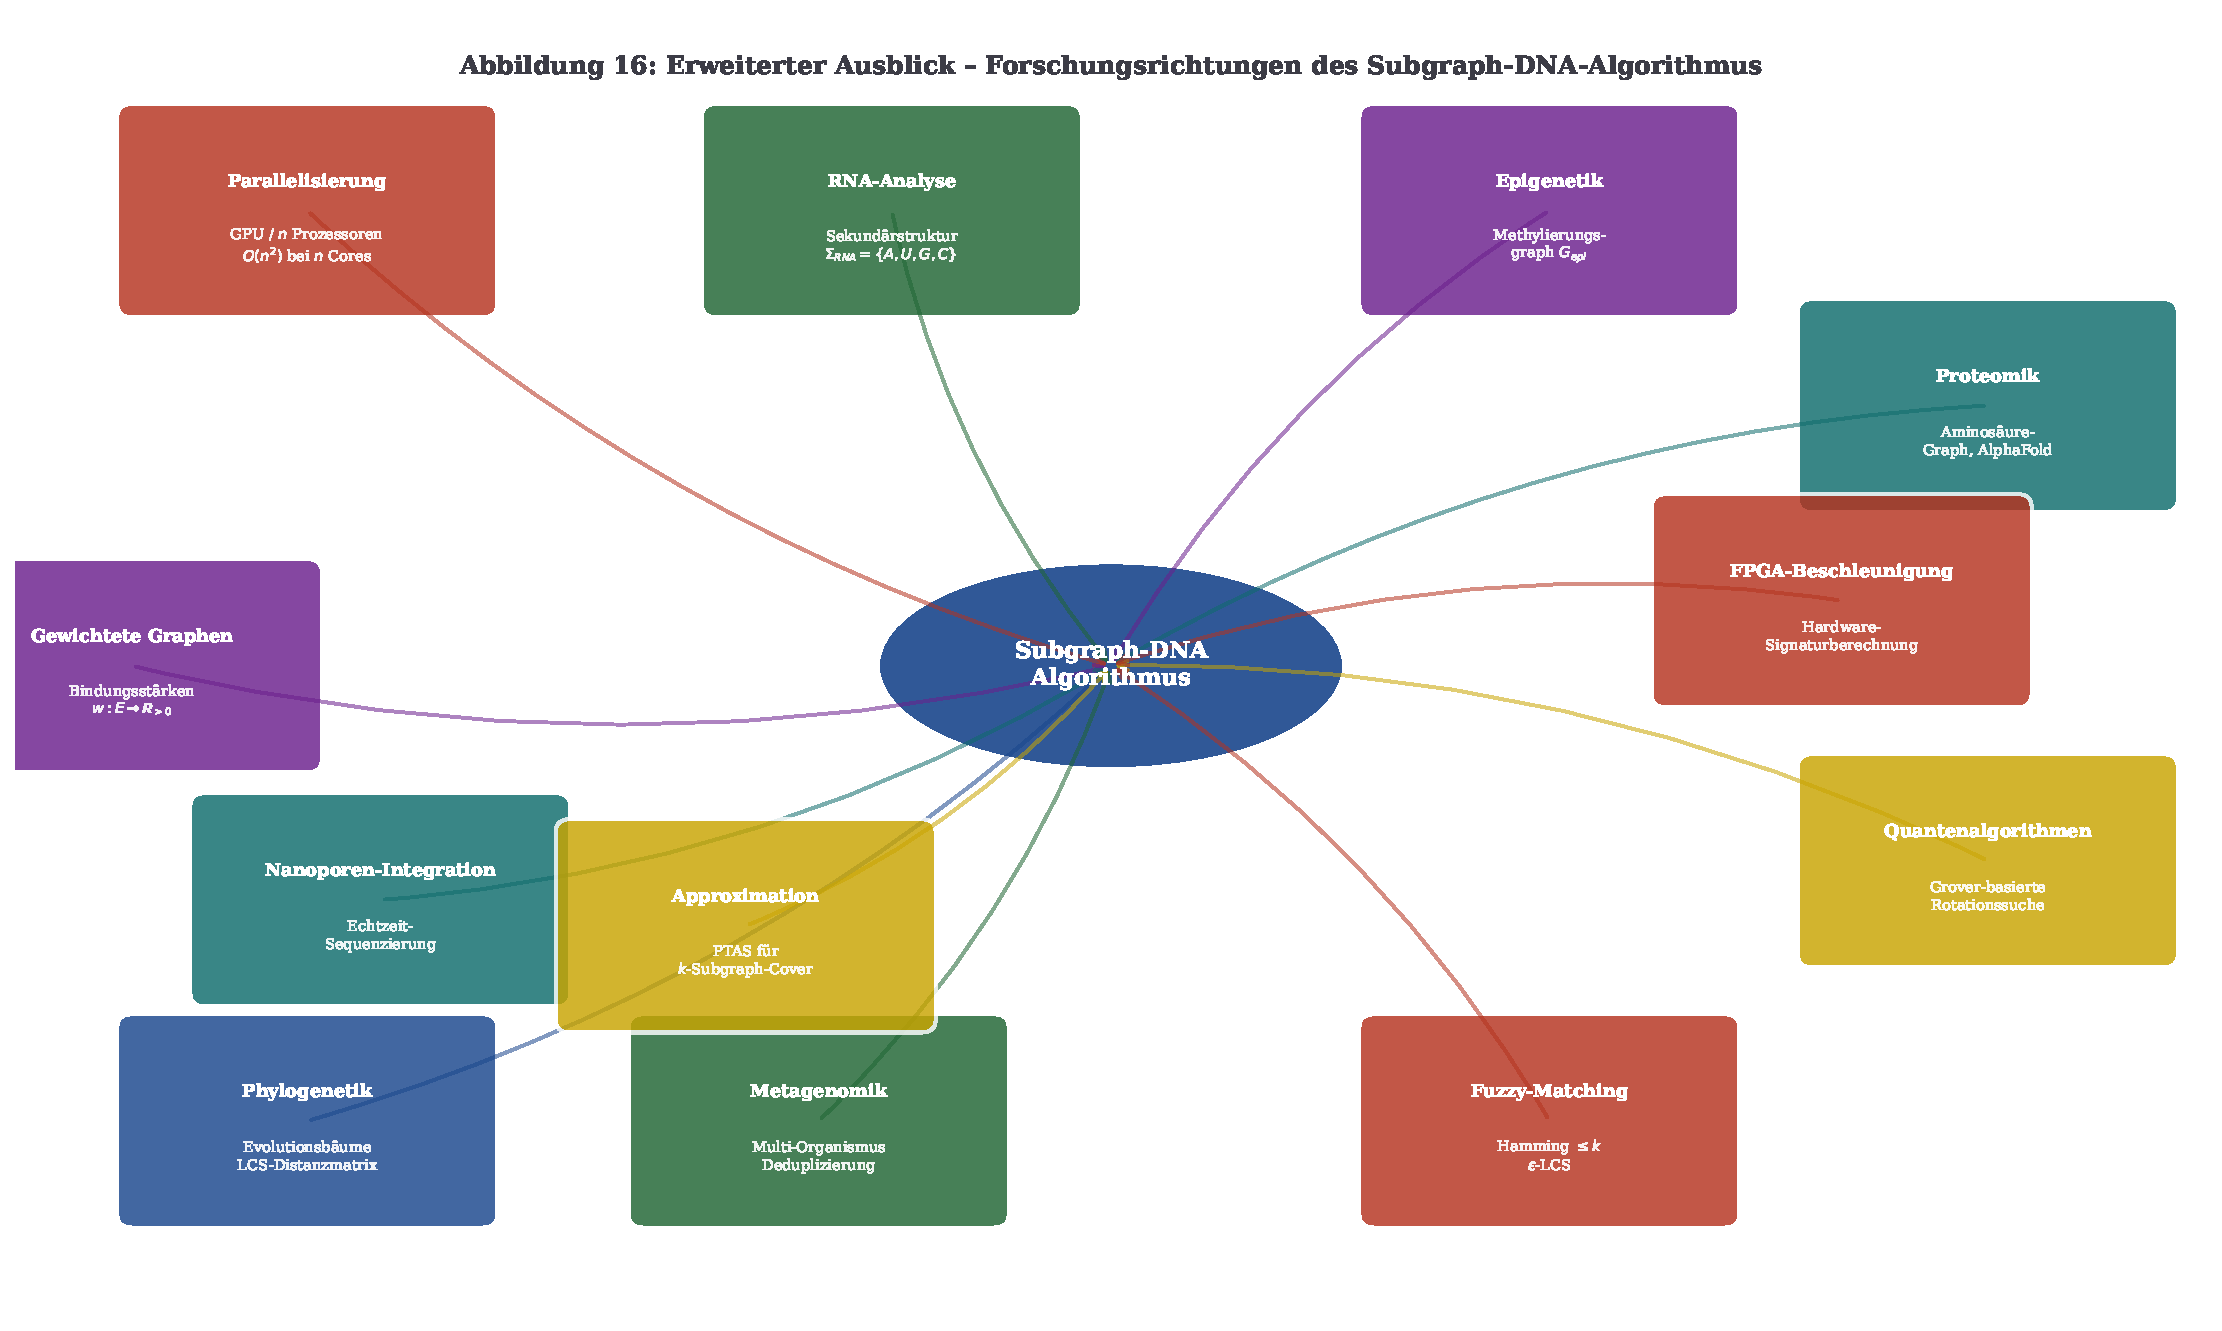
\includegraphics[width=0.95\textwidth]{figures/fig16_roadmap.pdf}
	\caption{Roadmap der Forschungsrichtungen des Subgraph-DNA-Algorithmus.
		Im Zentrum steht der Kernalgorithmus; die zwölf umgebenden Knoten
		repräsentieren konkrete Erweiterungsrichtungen, farblich nach Themengebiet
		gruppiert (blau = Algorithmus, grün = Biologie, rot = Anwendungen,
		lila = Hardware, türkis = benachbarte Disziplinen).}
	\label{fig:roadmap}
\end{figure}

\subsection{Implementierungshinweis}

Der Code des Subgraph Algorithmus ist verfügbar unter:
\url{https://github.com/hjstephan86/science}.

\begin{thebibliography}{9}
    \bibitem{epp2026}
    Stephan Epp.
    \textit{Der Subgraph Algorithmus}. 2026. Verfügbar auf
    \url{https://github.com/hjstephan86/science}

    \bibitem{watson1953}
    J.\,D. Watson und F.\,H.\,C. Crick.
    Molecular Structure of Nucleic Acids: A Structure for Deoxyribose
    Nucleic Acid.
    \textit{Nature}, 171:737--738, 1953.
    
    \bibitem{sanger1977}
    F. Sanger, S. Nicklen und A.\,R. Coulson.
    DNA sequencing with chain-terminating inhibitors.
    \textit{PNAS}, 74(12):5463--5467, 1977.
    
    \bibitem{abboud2015}
    A. Abboud, A. Backurs und V. Vassilevska Williams.
    Tight Hardness Results for LCS and Other Sequence Similarity Measures.
    \textit{FOCS 2015}, 2015.
    
    \bibitem{needleman1970}
    S.\,B. Needleman und C.\,D. Wunsch.
    A general method applicable to the search for similarities in the
    amino acid sequence of two proteins.
    \textit{J. Mol. Biol.}, 48(3):443--453, 1970.
    
    \bibitem{illumina2006}
    D.\,R. Bentley et al.
    Accurate whole human genome sequencing using reversible terminator
    chemistry.
    \textit{Nature}, 456:53--59, 2008.
    
    \bibitem{deamer2016}
    D. Deamer, M. Akeson und D. Branton.
    Three decades of nanopore sequencing.
    \textit{Nature Biotechnology}, 34:518--524, 2016.
    
    \bibitem{handelsman2004}
    J. Handelsman.
    Metagenomics: Application of Genomics to Uncultured Microorganisms.
    \textit{Microbiology and Molecular Biology Reviews}, 68(4):669--685, 2004.
    
    \bibitem{qin2010}
    J. Qin et al.
    A human gut microbial gene catalogue established by metagenomic sequencing.
    \textit{Nature}, 464:59--65, 2010.
    
    \bibitem{grover1996}
    L.\,K. Grover.
    A fast quantum mechanical algorithm for database search.
    \textit{STOC 1996}, 212--219, 1996.
    
    \bibitem{nussinov1980}
    R. Nussinov und A.\,B. Jacobson.
    Fast algorithm for predicting the secondary structure of single-stranded RNA.
    \textit{PNAS}, 77(11):6309--6313, 1980.
    
    \bibitem{neighbor_joining}
    N. Saitou und M. Nei.
    The neighbor-joining method: a new method for reconstructing phylogenetic trees.
    \textit{Molecular Biology and Evolution}, 4(4):406--425, 1987.

    % -------------------- Weitere Literatur (nicht zitiert) --------------------
    \bibitem{altschul1990}
    S. F. Altschul, W. Gish, W. Miller, E. W. Myers und D. J. Lipman.
    Basic local alignment search tool.
    \textit{J. Mol. Biol.}, 215(3):403--410, 1990.

    \bibitem{durbin1998}
    R. Durbin, S. Eddy, A. Krogh und G. Mitchison.
    Biological Sequence Analysis: Probabilistic Models of Proteins and Nucleic Acids.
    Cambridge University Press, 1998.

    \bibitem{li2013}
    H. Li.
    Aligning sequence reads, clone sequences and assembly contigs with BWA-MEM.
    \textit{arXiv:1303.3997}, 2013.

    \bibitem{langmead2009}
    B. Langmead, C. Trapnell, M. Pop und S. L. Salzberg.
    Ultrafast and memory-efficient alignment of short DNA sequences to the human genome.
    \textit{Genome Biology}, 10:R25, 2009.

    \bibitem{edgar2004}
    R. C. Edgar.
    MUSCLE: multiple sequence alignment with high accuracy and high throughput.
    \textit{Nucleic Acids Research}, 32(5):1792--1797, 2004.

    \bibitem{katoh2002}
    K. Katoh, K. Misawa, K. Kuma und T. Miyata.
    MAFFT: a novel method for rapid multiple sequence alignment based on fast Fourier transform.
    \textit{Nucleic Acids Research}, 30(14):3059--3066, 2002.

    \bibitem{bankevich2012}
    A. Bankevich et al.
    SPAdes: a new genome assembly algorithm and its applications to single-cell sequencing.
    \textit{J. Comput. Biol.}, 19(5):455--477, 2012.

    \bibitem{li2018}
    H. Li.
    Minimap2: pairwise alignment for nucleotide sequences.
    \textit{Bioinformatics}, 34(18):3094--3100, 2018.

    \bibitem{wood2019}
    D. E. Wood, J. Lu und B. Langmead.
    Improved metagenomic analysis with Kraken 2.
    \textit{Genome Biology}, 20:257, 2019.

    \bibitem{andrews2010}
    S. Andrews.
    FastQC: a quality control tool for high throughput sequence data.
    \textit{http://www.bioinformatics.babraham.ac.uk/projects/fastqc/}, 2010.

    \bibitem{cock2009}
    P. J. A. Cock et al.
    Biopython: freely available Python tools for computational molecular biology and bioinformatics.
    \textit{Bioinformatics}, 25(11):1422--1423, 2009.

    \bibitem{mcclintock1950}
    B. McClintock.
    The origin and behavior of mutable loci in maize.
    \textit{PNAS}, 36(6):344--355, 1950.

    \bibitem{felsenstein1985}
    J. Felsenstein.
    Confidence limits on phylogenies: an approach using the bootstrap.
    \textit{Evolution}, 39(4):783--791, 1985.

    \bibitem{staden1979}
    R. Staden.
    A strategy of DNA sequencing employing computer programs.
    \textit{Nucleic Acids Research}, 6(7):2601--2610, 1979.

    \bibitem{pevzner2001}
    P. A. Pevzner, H. Tang und M. S. Waterman.
    An Eulerian path approach to DNA fragment assembly.
    \textit{PNAS}, 98(17):9748--9753, 2001.

    \bibitem{myers2000}
    E. W. Myers et al.
    A whole-genome assembly of Drosophila.
    \textit{Science}, 287(5461):2196--2204, 2000.

    \bibitem{kent2002}
    W. J. Kent.
    BLAT—the BLAST-like alignment tool.
    \textit{Genome Research}, 12(4):656--664, 2002.

    \bibitem{benson2013}
    D. A. Benson et al.
    GenBank.
    \textit{Nucleic Acids Research}, 41(D1):D36--D42, 2013.

    \bibitem{bairoch2000}
    A. Bairoch und R. Apweiler.
    The SWISS-PROT protein sequence database and its supplement TrEMBL.
    \textit{Nucleic Acids Research}, 28(1):45--48, 2000.

    \bibitem{eddy2011}
    S. R. Eddy.
    Accelerated Profile HMM Searches.
    \textit{PLoS Comput Biol}, 7(10):e1002195, 2011.

    \bibitem{smith1981}
    T. F. Smith und M. S. Waterman.
    Identification of common molecular subsequences.
    \textit{J. Mol. Biol.}, 147(1):195--197, 1981.

    \bibitem{fitch1967}
    W. M. Fitch und E. Margoliash.
    Construction of phylogenetic trees.
    \textit{Science}, 155(3760):279--284, 1967.

    \bibitem{wilbur1983}
    W. J. Wilbur und D. J. Lipman.
    Rapid similarity searches of nucleic acid and protein data banks.
    \textit{PNAS}, 80(3):726--730, 1983.

    \bibitem{lander2001}
    E. S. Lander et al.
    Initial sequencing and analysis of the human genome.
    \textit{Nature}, 409:860--921, 2001.

    \bibitem{venter2001}
    J. C. Venter et al.
    The sequence of the human genome.
    \textit{Science}, 291(5507):1304--1351, 2001.

    \bibitem{margulies2005}
    M. Margulies et al.
    Genome sequencing in microfabricated high-density picolitre reactors.
    \textit{Nature}, 437:376--380, 2005.

    \bibitem{eid2009}
    J. Eid et al.
    Real-time DNA sequencing from single polymerase molecules.
    \textit{Science}, 323(5910):133--138, 2009.

    \bibitem{ron2011}
    R. Shamir et al.
    EXPANDER -- an integrative program suite for microarray data analysis.
    \textit{BMC Bioinformatics}, 6:232, 2005.

    \bibitem{waterman1984}
    M. S. Waterman.
    General methods of sequence comparison.
    \textit{Bull. Math. Biol.}, 46(4):473--501, 1984.

    \bibitem{krogh1994}
    A. Krogh, M. Brown, I. S. Mian, K. Sjölander und D. Haussler.
    Hidden Markov models in computational biology: applications to protein modeling.
    \textit{J. Mol. Biol.}, 235(5):1501--1531, 1994.

    \bibitem{fleischmann1995}
    R. D. Fleischmann et al.
    Whole-genome random sequencing and assembly of \textit{Haemophilus influenzae} Rd.
    \textit{Science}, 269(5223):496--512, 1995.

    \bibitem{salzberg2012}
    S. L. Salzberg et al.
    GAGE: a critical evaluation of genome assemblies and assembly algorithms.
    \textit{Genome Research}, 22(3):557--567, 2012.

    \bibitem{miller2010}
    J. R. Miller, S. Koren und G. Sutton.
    Assembly algorithms for next-generation sequencing data.
    \textit{Genomics}, 95(6):315--327, 2010.
    % --------------------------------------------------------------------------

\end{thebibliography}

\end{document}
